% 物联网
% 物联网.tex

\documentclass[12pt,UTF8]{ctexbook}

% 设置纸张信息。
\usepackage[a4paper,twoside]{geometry}
\geometry{
	left=25mm,
	right=25mm,
	bottom=25.4mm,
	bindingoffset=10mm
}

% 设置字体,并解决显示难检字问题。
\xeCJKsetup{AutoFallBack=true}
\setCJKmainfont{SimSun}[BoldFont=SimHei, ItalicFont=KaiTi, FallBack=SimSun-ExtB]

% 目录 chapter 级别加点(.)。
\usepackage{titletoc}
\titlecontents{chapter}[0pt]{\vspace{3mm}\bf\addvspace{2pt}\filright}{\contentspush{\thecontentslabel\hspace{0.8em}}}{}{\titlerule*[8pt]{.}\contentspage}

% 设置 part 和 chapter 标题格式。
\ctexset{
	chapter/name={第,章},
	chapter/number={\arabic{chapter}}
}

% 图片相关设置。
\usepackage{graphicx}
\graphicspath{{Images/}}

% 设置署名格式。
\newenvironment{shuming}{\hfill\zihao{4}}

% 注脚每页重新编号,避免编号过大。
\usepackage[perpage]{footmisc}

\title{\heiti\zihao{0} 物联网}
\author{佚名}
\date{}

\begin{document}

\maketitle
\tableofcontents

\frontmatter

\mainmatter

\chapter{物联网的基础知识}

首先我们来了解一下学习物联网所需的基础知识。

\section{物联网入门}

\subsection{物联网}

大家在听到物联网时,脑海中会出现一个什么样的印象呢?

物联网的英语是 Internet of Things,缩写为 IoT,这里的“物”指的是我们身边一切能与网络相连的物品。例如您身上穿着的衣服、戴着的手表、家里的家用电器和汽车,或者是房屋本身,甚至正在读的这本书,只要能与网络相连,就都是物联网说的“物”。

就像我们用互联网在彼此之间传递信息一样,物联网就是“物”之间通过连接互联网来共享信息并产生有用的信息,而且无需人为管理就能运行的机制。这样一来,就创造出了一直未能实现的魔法般的世界。

\subsection{物联网的相关动向}

ICT\footnote{信息、通信和技术三个英文单词的首字母组合(Information Communication Technology,简称 ICT)。} 市场调查公司的 IDC(Internet Data Center,互联网数据中心)调查结果显示,2013 年日本国内物联网市场的市场份额约有 11 万亿日元,预测这个数字在 2018 年大约会增至 2013 年的两倍,即 21 万亿日元左右。

物联网市场是由若干个市场形成的,包括作为“物”的设备市场,掌管物与物之间联系的网络市场,还有运营管理类的平台市场,分析采集到的数据的分析处理市场等(图 1.1)。

\begin{figure}[htbp]
	\centering
	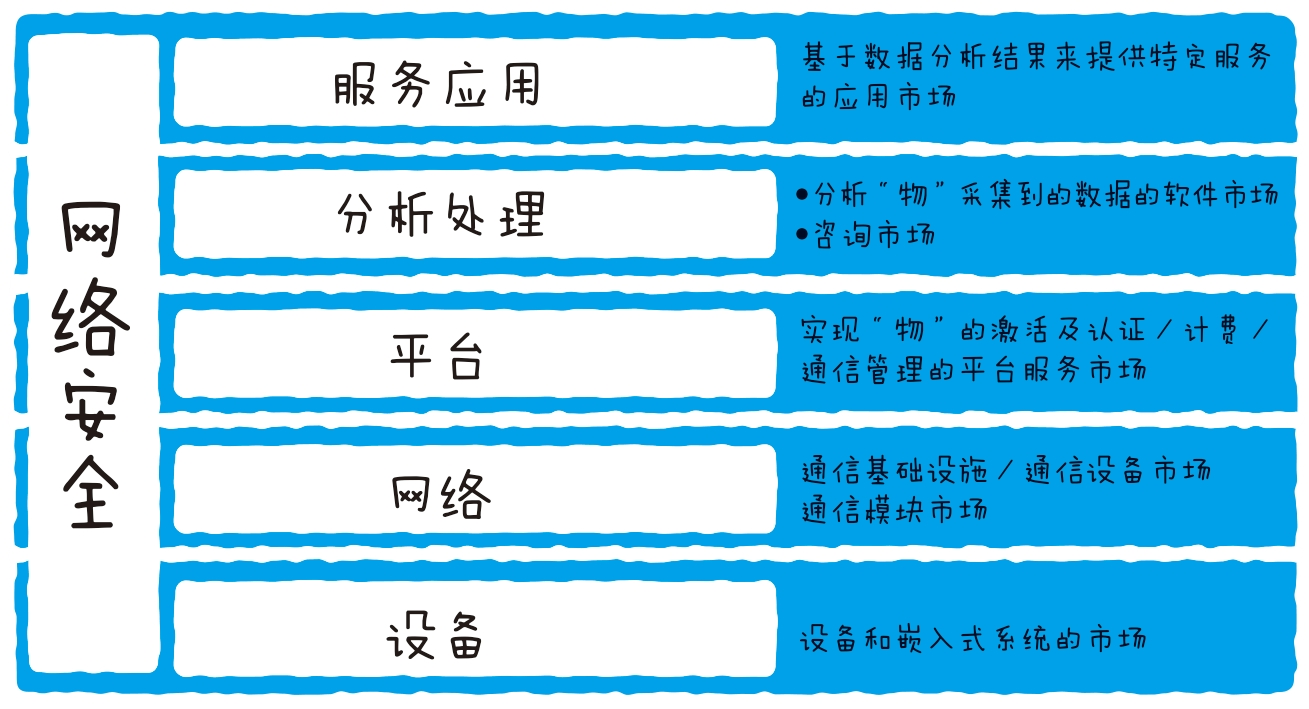
\includegraphics[width=1\linewidth]{1}
	\caption{物联网的相关市场}
	\label{fig:1}
\end{figure}

说起创建物联网市场的要素,那就要提到通信模块价格趋向低廉以及云服务的普及。英特尔公司在 2014 年 10 月将一款名为英特尔 Edison 的单板计算机投入了市场。这款单板机在一个只有邮票大小的模块上搭
载了双核双线程的 CPU 和 1 GB 内存、4 GB 的存储空间、双频的 Wi-Fi 以及蓝牙 4.0。除此之外,微软还公布了名为 Microsoft Azure Intelligent Systems Service(Azure 智能系统服务)的解决方案,它负责用云技术实现数据管理和处理,以及通信管理等功能。

此外,在平台、分析处理和网络安全等方面,针对物联网的产品和服务也已经开始投入市场。物联网市场今后的重点在于跟熟悉各垂直市场的从业者加强合作,积极提供试验环境以及开发贴近用户生活的服务项目。

\section{物联网所实现的世界}

\subsection{“泛在网络”社会}

在讲物联网所实现的世界之前,我们先从“连接网络”的观点来回顾一下历史。

20 世纪 90 年代初,过去以大型机为中心的集中式处理逐渐向以客户端服务器为中心的分布式处理转移。自 20 世纪 90 年代后期起,新型集中式处理围绕着以互联网和 Web 为代表的网络形成了一股发展趋势。这就是 Web 计算的概念。以互联网为媒介,人们可以轻松实现 PC、服务器、移动设备之间的信息交换。

21世纪初,一个名为“泛在网络”的概念开始受到人们的关注。泛在网络的理念在于使人们能够通过“随时随地”连接互联网等网络来利用多种多样的服务(图 1.2)。近年来,通过智能手机和平板电脑,甚至游戏机、电视机等一些过去无法连接到网络的“物”,就可以随时随地访问互联网。

\begin{figure}[htbp]
	\centering
	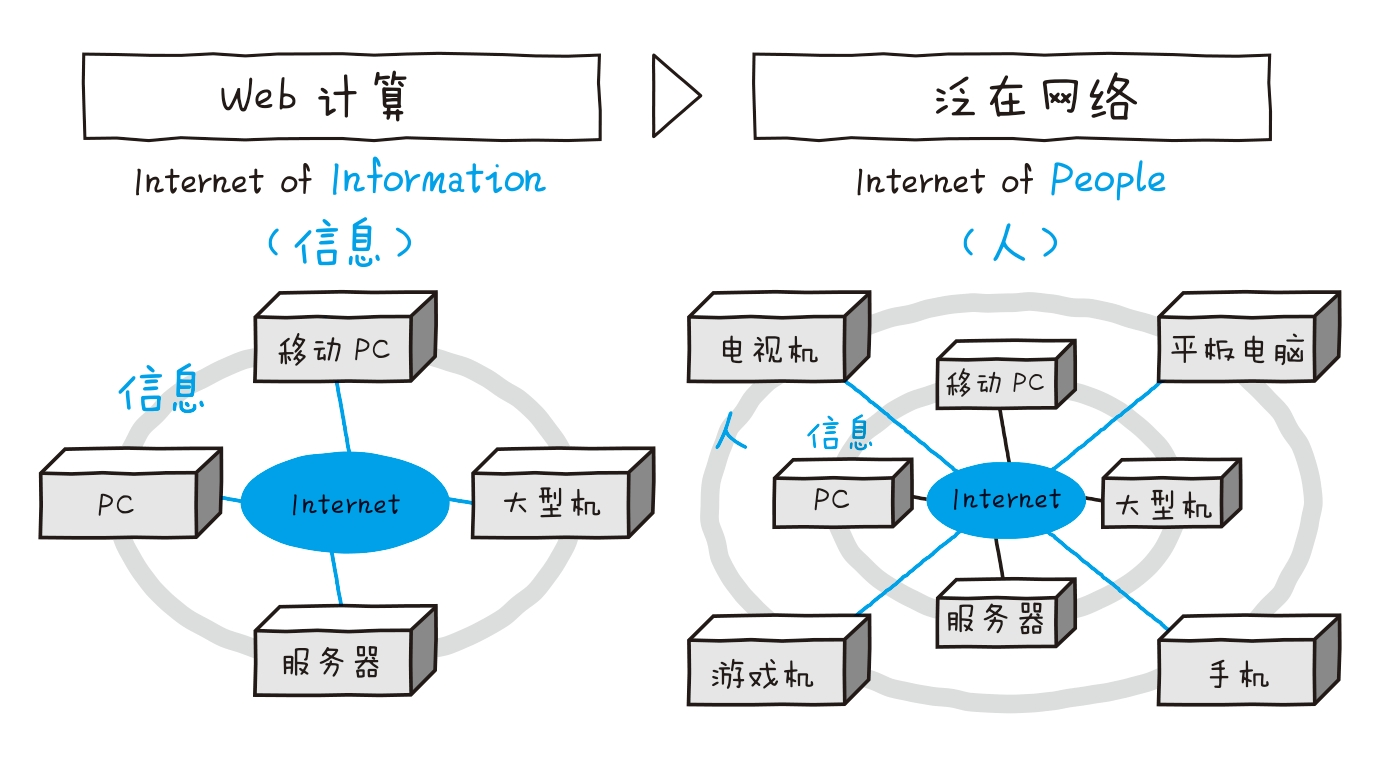
\includegraphics[width=1\linewidth]{2}
	\caption{泛在网络可以让人们随时随地访问网络}
	\label{fig:1}
\end{figure}

\subsection{“物”的互联网连接}

随着宽带的普及,泛在网络社会日益得到实现。此外,能搭载在机器上的超低功耗传感器投入市场、无线通信技术进步等,都促使除了电脑、服务器和智能手机等传统连接互联网的 IT 相关设备以外,各种各样的“物”也可以连接互联网(图 1.3)。以汽车、家用电器以及房屋为开端,近来,眼镜和手表、饰品这些戴在身上的“物”也连接上了互联网并开始得到应用,如 Google Glass 和 Apple Watch 。

\begin{figure}[htbp]
	\centering
	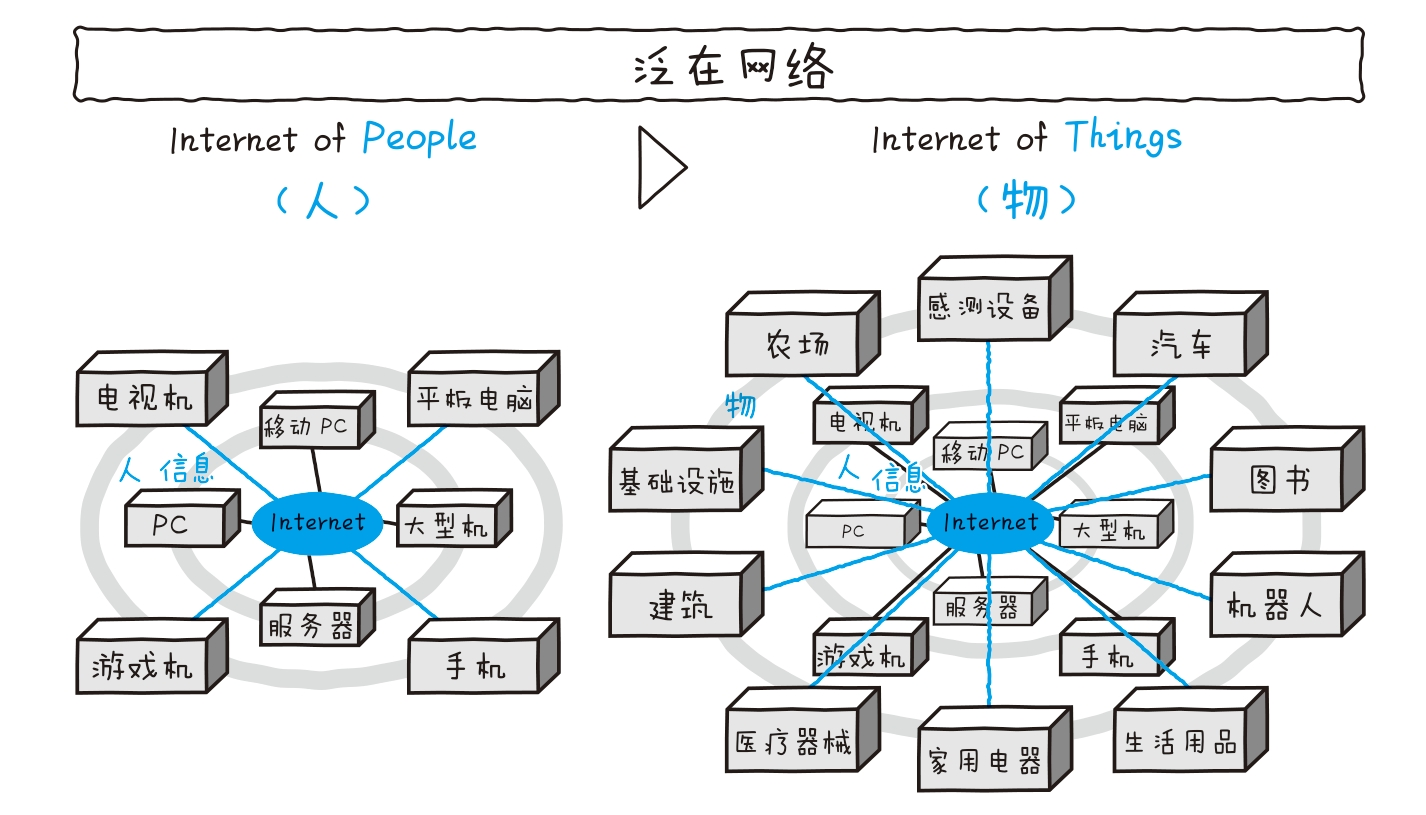
\includegraphics[width=1\linewidth]{3}
	\caption{连接互联网的各种各样的“物”}
	\label{fig:1}
\end{figure}

形形色色的“物”都能与互联网相连,这一点大家都已经了解了。那么这种“相连”会产生什么呢?它又是如何给人们的生活带来方便的呢?下面,就来看看物联网带给我们的世界吧。

\subsection{机器对机器通信所实现的事}

在物联网的实现方面,近年来机器对机器通信等关键技术备受人们关注(图 1.4)。物联网和机器对机器通信在很多方面可以视作同一个意思,但从严格意义上来说二者是不同的。机器对机器通信是不经人为控制的、机器和机器之间的通信;也就是说,多数情况下它表示的是机器和机器自动交换信息的整体系统。另一方面,物联网则大多含有给信息接收者提供服务的含义,它比机器对机器通信的概念范围更广。

\begin{figure}[htbp]
	\centering
	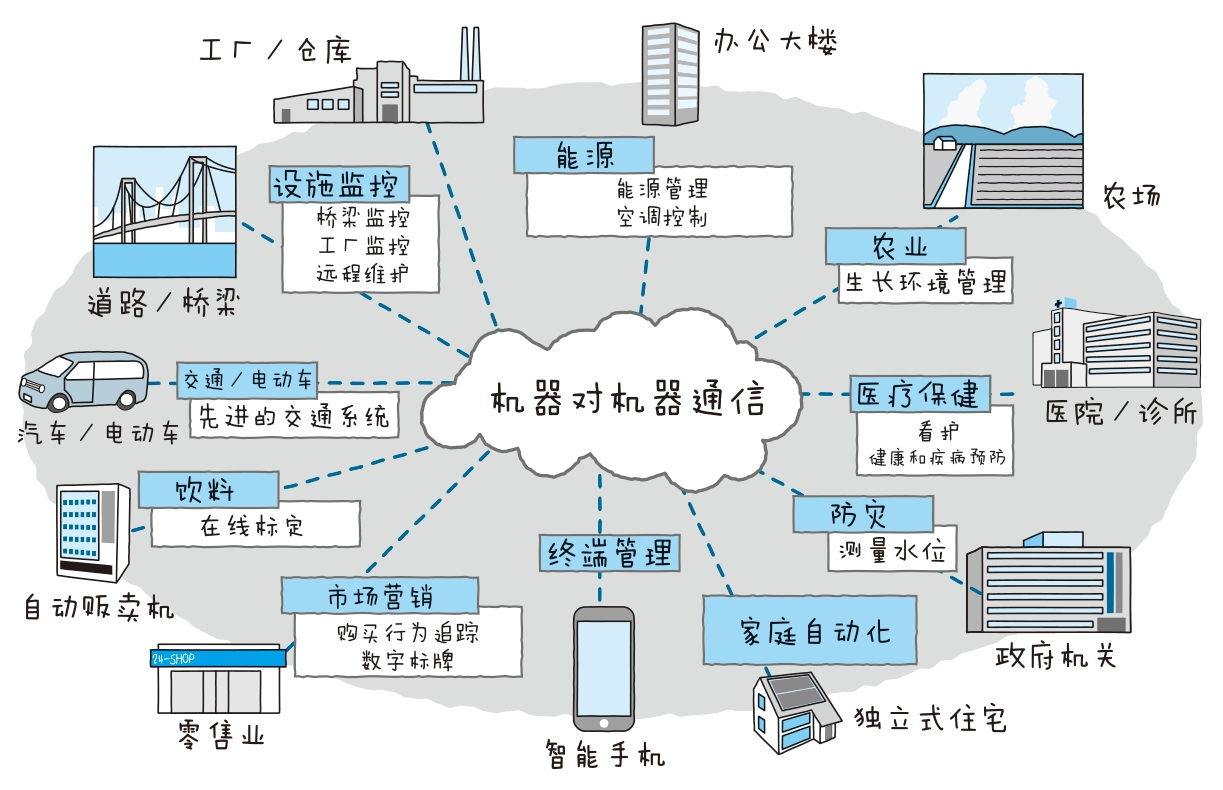
\includegraphics[width=1\linewidth]{4}
	\caption{机器对机器通信所实现的社会}
	\label{fig:1}
\end{figure}

泛在计算的世界是一个所有的“物”都内置计算机中,随时随地可以得到计算机帮助的世界。而机器对机器通信支撑着泛在计算的世界,并通过支撑社会的基础设施——智能社区和智能电网等形式逐步得到实现。

此外,机器对机器通信不仅可以通过 3G 和 LTE 电路的信息系统实现,还可以通过本地网络中的无线通信和有线通信来实现。

除了企业内的信息和互联网的信息以外,我们还能够灵活应用来自机器的信息。这样一来也就掌握了现实世界中的情况变动,尤其是提高了企业中的信息应用度。

\subsection{物联网实现的世界}

大家已经知道,我们可以借助机器对机器通信采集和积累信息,并灵活运用从信息中分析出的数据来方便我们的生活。那么,如果在此基础上把数百亿台设备都连接上物联网,又会如何呢?

以前,人们通过让少数昂贵的工业机械通信,来实现对“物”的远程控制。今后,人们将更多地以低廉的价格大量生产面向用户的机器,并让这些机器通信。也正因应用了从这些“物”中获取的数据,各种各样的服务才如雨后春笋般涌现出来。此外,先进感测技术的普及实现了人类对现实世界的掌握和预测,通过实时且海量地搜集人、物、社会和环境的数据,也有望进行新型社会基础设施的构建,例如强化产业竞争力、建设都市和社会制度、监测灾害等异常情况。

除了那些一眼就能看明白的设备,具有连通性(机器和系统间的互联性和关联性)的设备也在不断地随处增加。物联网的趋势指的就是这一现象。通过本章,我们再深入地看一下物联网所实现的是一个怎样的世界。

1. 智能设备

2. 具备连通性的“物”

3. 网络

4. Web 系统

5. 数据分析技术

大家认为把这些因素组合到一起,将会产生出一个怎样的充满革新性的服务呢?

举个例子,市面上已经出现了很多叫作智能家居的设备,其用途是控制智能住宅。飞利浦 Hue 是一款能通过 IP 网络来控制自身亮度和光色的灯泡。Nest 是一种机器控制器,它能学习如何控制空调等机器以及如何设定这些机器的目标值。如果把它们与 Web 系统和可穿戴设备等智能设备组合在一起,还能实现由住宅主动根据人的动作和身体状况来调整环境(图 1.5)。

\begin{figure}[htbp]
	\centering
	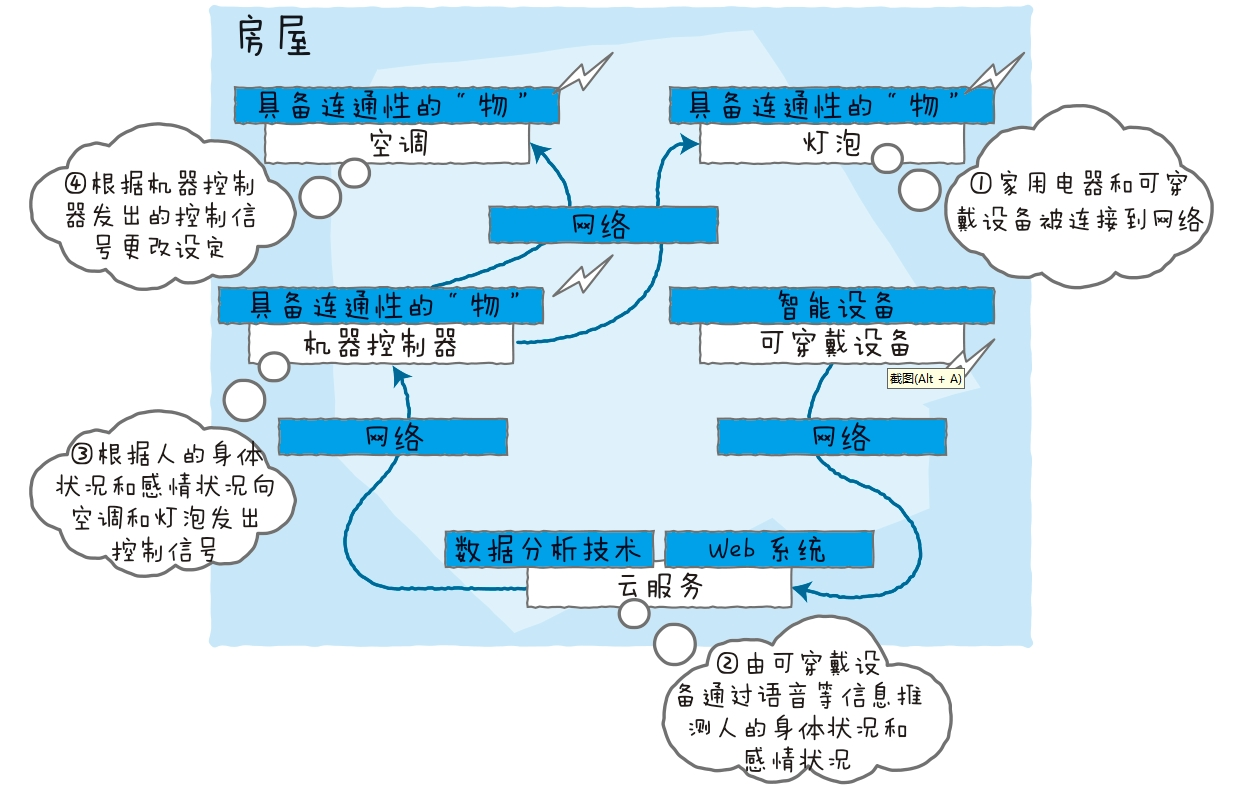
\includegraphics[width=1\linewidth]{5}
	\caption{根据人体状况自动控制环境——以智能家居为例}
	\label{fig:1}
\end{figure}

可以说,当下的趋势之一就是不停留在单纯的控制层面,而是像“凭借短距离通信实现自主控制和自动化”及“通过机器学习实现自动判断”这样,给事物增添附加价值。

\subsection{蓬勃发展的标准化活动}

除 IETE\footnote{The Institution of Electronics and Telecommunication Engineers
电子与电信工程师协会。} 、3GPP\footnote{Third Generation Partnership Project
第三代合作伙伴计划。} 、ITU\footnote{International Telecommunication Union
国际电信联盟。} 等标准化团体以外,民间企业也围绕物联网积极地开展了活动。

2013 年 12 月,在美国高通公司的支持下,家电厂商的横向性物联网推进联盟 AllSeen Alliance 成立了。该联盟的意图在于越过厂商这道高墙,规划一种统一规格,让冰箱、烤箱及电灯等所有电器都能通过互联网实现协作。

2014 年 7 月,在英特尔和三星的推动下,物联网联盟 OIC\footnote{Open Interconnect Consortium
开放互联联盟。} 成立了。该联盟旨在为物联网相关机器的规格和认证设立标准。

可想而知,今后物联网普及的关键在于各厂商是否采用这种开放性规格。作为从事物联网的工程师,在选定产品时还得把这种标准化动向考虑进去,这一点是重中之重。

\section{实现物联网的技术要素}

要实现物联网,需要很多技术要素。除了传感器等电子零件和电子电路以外,还包括 Web 应用中经常用到的技术,以及数据分析等。本书将会为大家整体解说这些技术。个别详细内容在第 2 章及以后的章节中会提到,这里我们先来总览一下本书将会讲解的全部内容。

\subsection{设备}

物联网与以往的 Web 服务不同,设备在其中担任着重要的作用。设备指的是一种“物”,它上面装有一种名为传感器的电子零件,并与网络相连接。比如大家拿着的智能手机和平板电脑就是设备的一种。家电产品、我们时刻戴着的手表以及伞等,只要能满足上述条件,就是设备(图 1.6)。

\begin{figure}[htbp]
	\centering
	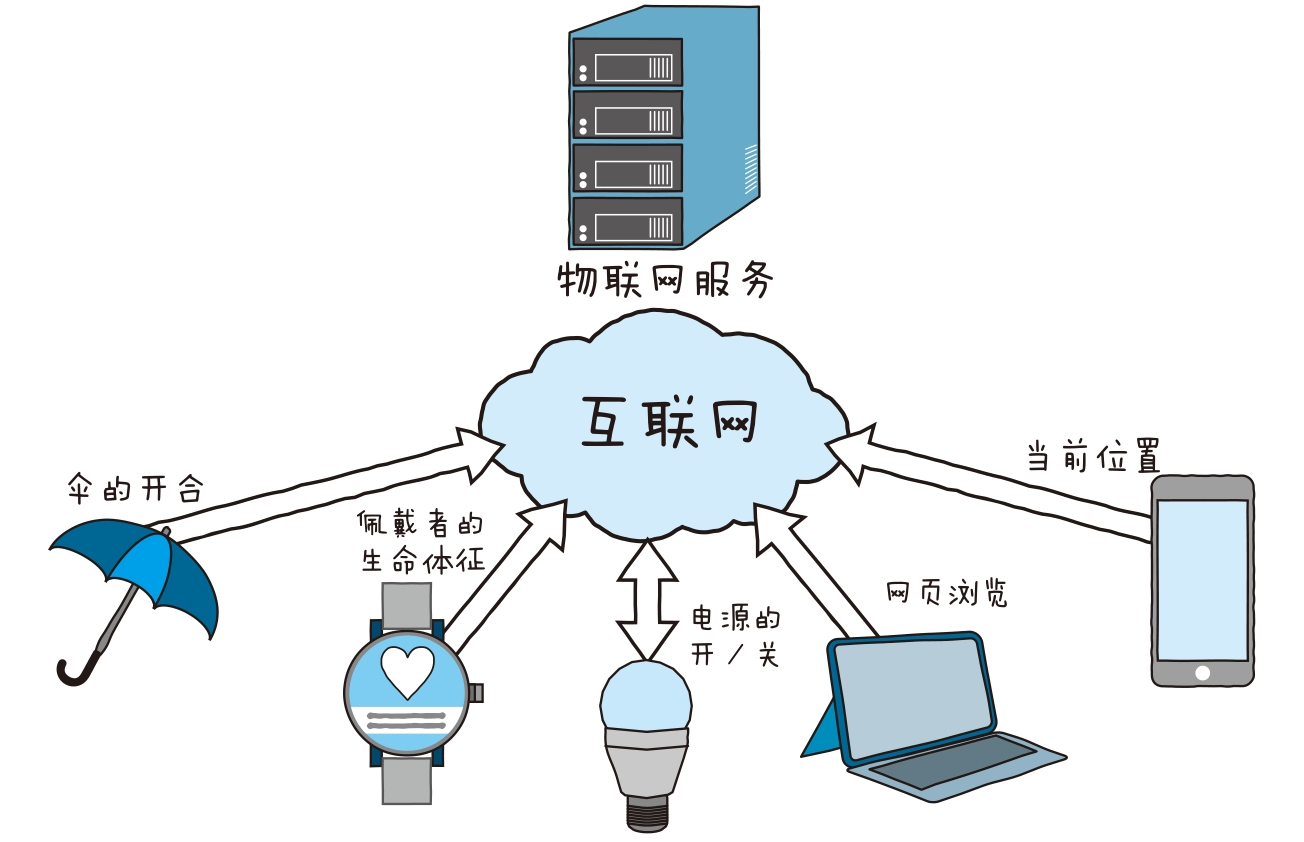
\includegraphics[width=1\linewidth]{6}
	\caption{与网络连接的设备}
	\label{fig:1}
\end{figure}

这些设备起着两个作用:感测和反馈。下面我们分别说明它们各自的作用。

\subsubsection{感测的作用}

感测指的是搜集设备本身的状态和周边环境的状态并通知系统(图 1.7)。这里说的状态包括房门的开闭状态、房间的温度和湿度、房间里面有没有人,等等。设备是利用传感器这种电子零件来实现感测的。

打个比方,如果伞上有用于检测其开合的传感器并具备连接网络的功能,那么多把伞的开合状态就可以被检测到。利用这一点就能调查出是否在下雨。在这种情况下,如果一个地区有多把伞打开,就可以推测出该地区正在下雨。反过来,就能推断出大多数伞都合着的地区没有在下雨。此外,通过感测设备周边的环境还能搜集温度和湿度等信息。

\begin{figure}[htbp]
	\centering
	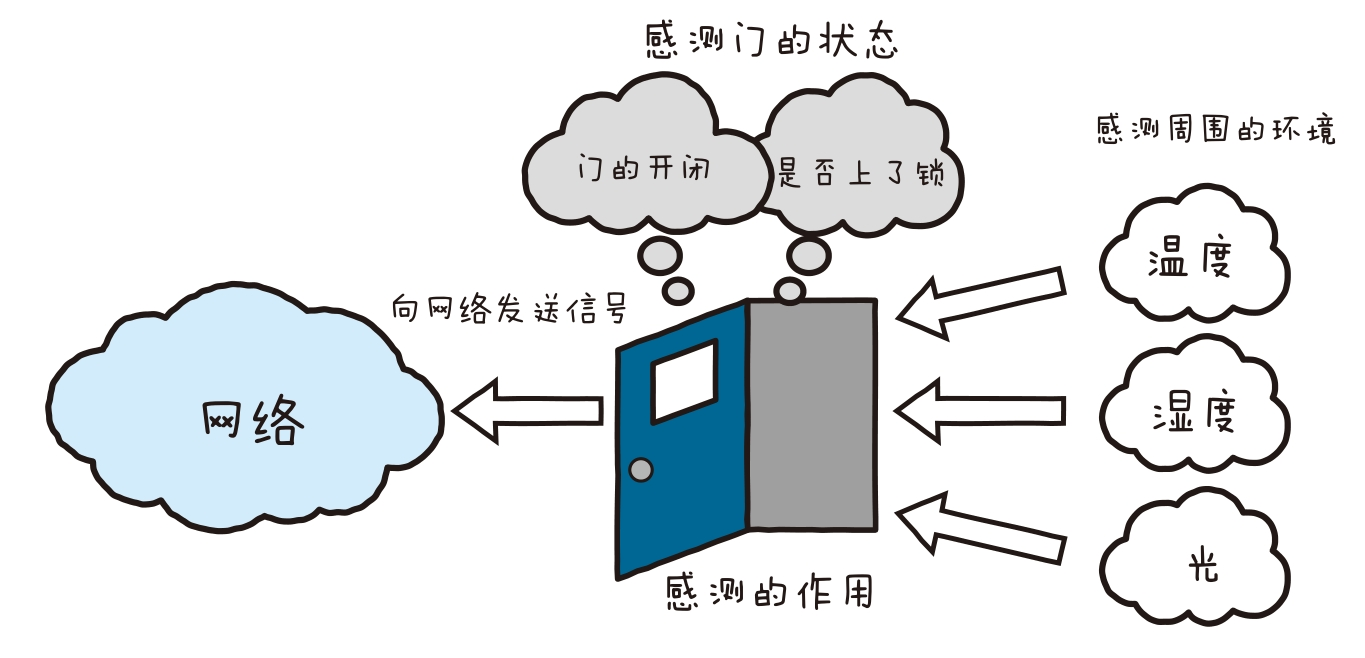
\includegraphics[width=1\linewidth]{7}
	\caption{感测的作用}
	\label{fig:1}
\end{figure}

\subsubsection{反馈的作用}

设备的另外一个作用是接收从系统发来的通知,显示信息或执行指定操作(图 1.8)。系统会基于从传感器处搜集到的信息进行一些反馈,并针对现实世界采取行动。

\begin{figure}[htbp]
	\centering
	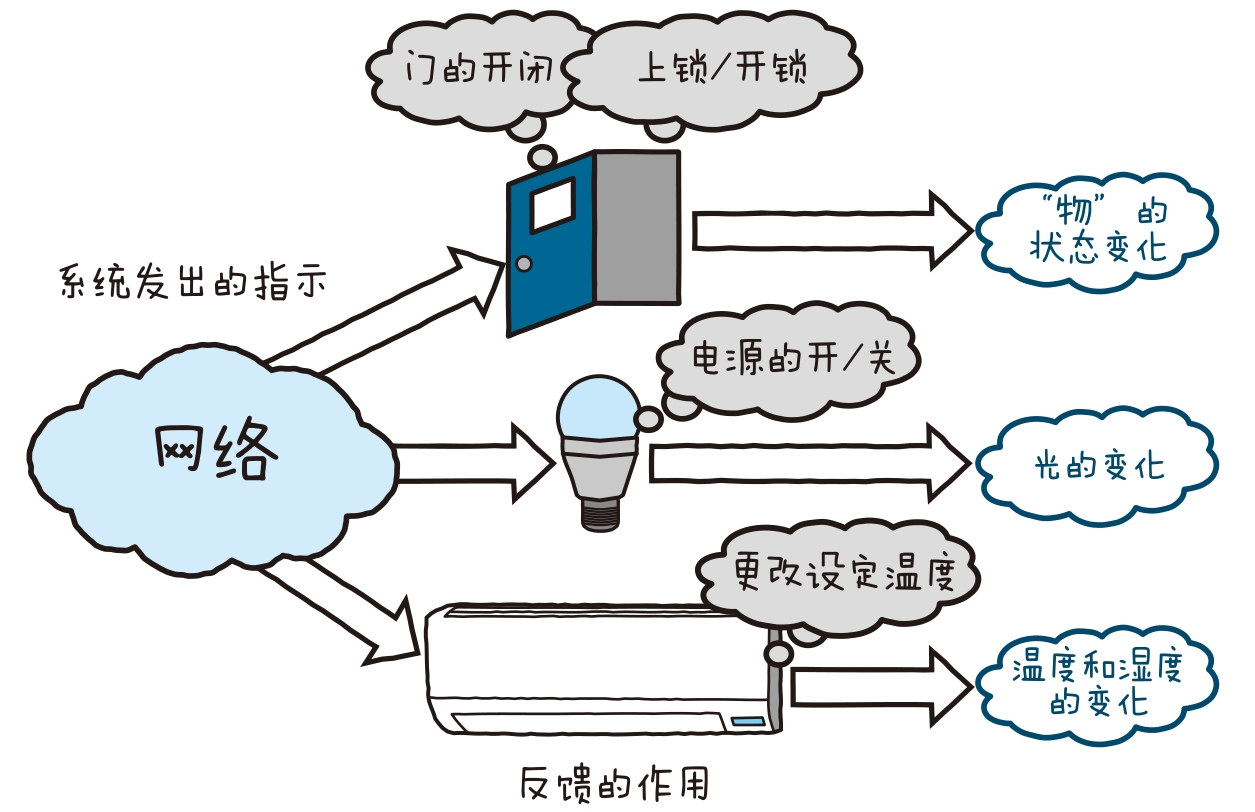
\includegraphics[width=1\linewidth]{8}
	\caption{反馈的作用}
	\label{fig:1}
\end{figure}

反馈有多种方法。大体分成如图 1.9 所示的 3 种方法,分别是可视化、通知,以及控制。

\begin{figure}[htbp]
	\centering
	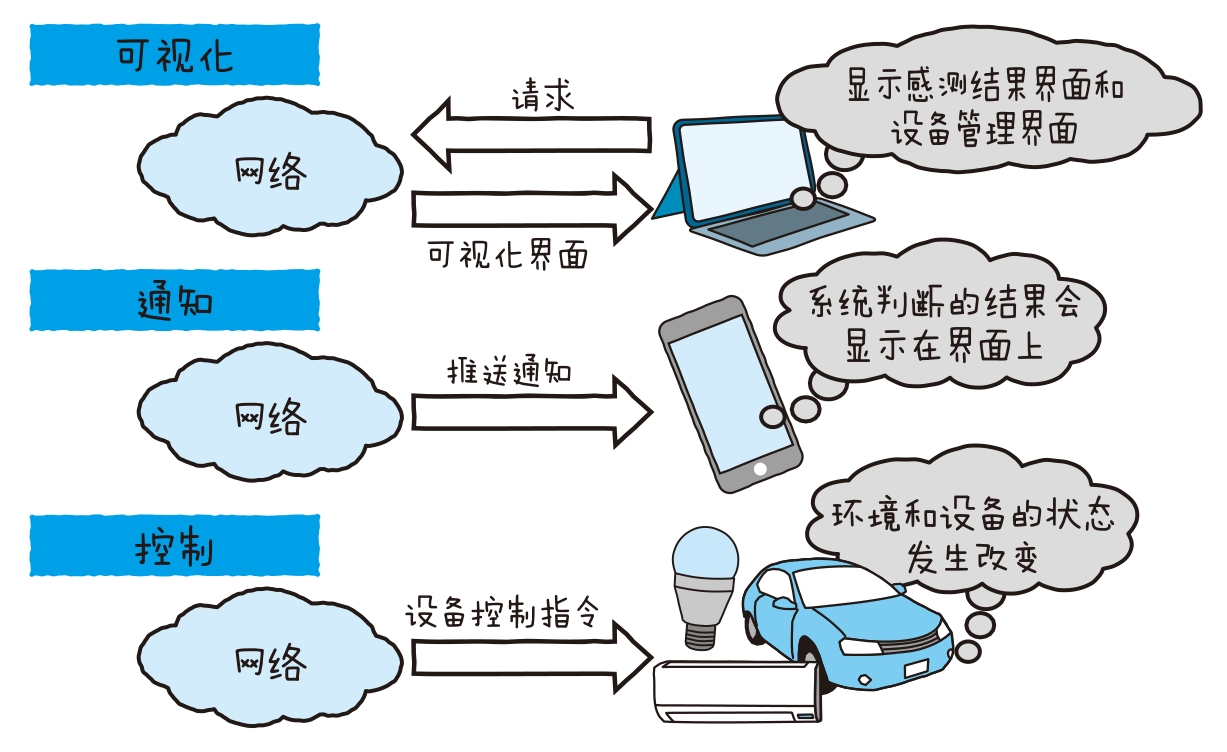
\includegraphics[width=1\linewidth]{9}
	\caption{反馈的 3 种方法}
	\label{fig:1}
\end{figure}

比方说,用户通过“可视化”就能使用电脑和智能手机上的 Web 浏览器浏览物联网服务搜集到的信息。虽然最终采取行动的是用户,不过这是最简单的一个反馈的例子。只要把房间的当前温度和湿度可视化,人就能将环境控制在最适宜的条件下。

利用“推送通知”,系统就能检测到“物”的状态和某些活动,并将其通知给设备。例如从服务器给用户的智能手机推送通知,使其显示消息。近年来,Facebook 和 Twitter 等 SNS 社交应用就在贴心地向我们的智能手机频繁推送朋友们吃饭和旅行的消息。如果你去逛超市时,推送通知能告诉你冰箱的牛奶过了保质期,洗涤用品卖完了,这个世界岂不就更方便了吗?

利用“控制”,系统就可以直接控制设备的运转,而无需借助人工。假设在某个夏天的傍晚,你正在从离家最近的车站往家走,你的智能手机会用 GPS 确定你现在的位置和前进的方向,用加速度传感器把你的步速通知给物联网服务。这样一来,服务就能分析出你正在回家的路上,进而从你的移动速度预测你到家的时间,然后发出指示调节家里空调的温度并令其开始运转。这样当你回到家的时候,家里就已经很舒服了。

\subsection{传感器}

要想像前文说的那样搜集设备和环境的状态,就需要利用一个叫作传感器的电子零件。

传感器负责把物理现象用电子信号的形式输出。例如有的传感器可以把温度和湿度作为电子信号输出,还有的传感器能把超声波和红外线等人类难以感知的现象转换成电子信号输出。

数码相机上使用的图像传感器也能把进入镜头的光线捕捉成 3 种颜色的光源,并将其转换成电子信号。因此它也可以归在传感器的分类里。传感器的种类如图 1.10 所示。关于这些传感器的种类和它们各自的结构,我们会在第 3 章详细介绍。

\begin{figure}[htbp]
	\centering
	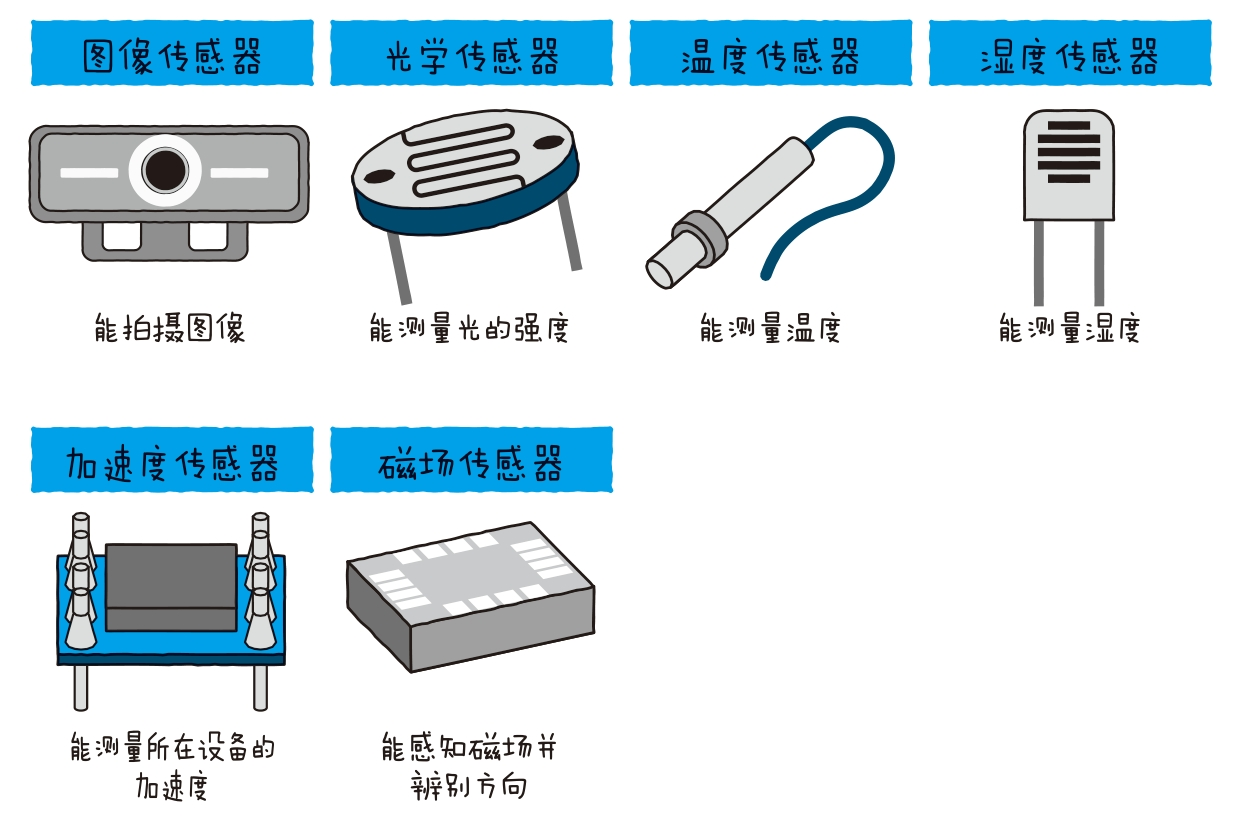
\includegraphics[width=1\linewidth]{10}
	\caption{具有代表性的传感器的种类}
	\label{fig:1}
\end{figure}

通过传感器输出的电子信号,系统就能够获取现实世界的“物”的状态和环境的状态。

人们很少单独利用这些传感器,通常都是将它们置入各种各样的“物”里来加以利用。最近的智能手机和平板电脑就内置了很多传感器,例如用于检测画面倾斜度的陀螺仪传感器和加速度传感器,采集语音的麦克风,用于拍摄照片的相机,具备指南针功能的磁场传感器。

还有一种东西叫作传感器节点,它把传感器本身置入环境中搜集信息。传感器节点是集蓝牙和 Wi-Fi 等无线通信装置与电池为一体的传感器。我们把这些传感器连接到一种叫作网关的专用无线路由器来进行传感器数据的搜集(图 1.11)。

\begin{figure}[htbp]
	\centering
	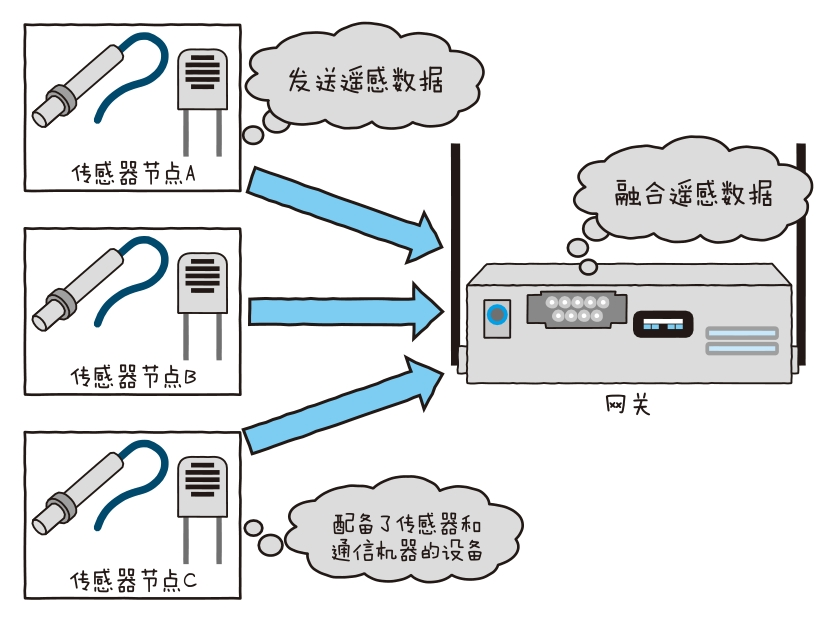
\includegraphics[width=1\linewidth]{11}
	\caption{传感器节点和网关}
	\label{fig:1}
\end{figure}

比如,在农场测量栽培植物的环境时,或是检测家里房间的温度和湿度时,就可以利用这些传感器节点。除此之外,市面上还有各种各样用于医疗保健的可穿戴设备,这些设备上装有加速度传感器和脉搏计,人们可以利用这些设备管理自己的生活节奏和健康状况。

这样一来,物联网服务就能利用传感器获取设备、环境、人这些“物”的状态。自己想实现的服务都需要哪些信息,为此应该利用哪种传感器和设备,这些都需要我们仔细分析。

\subsection{网络}

在把设备连接到物联网服务时,网络是不可或缺的。不仅要把设备连接到物联网服务,还得把设备连接到其他设备。物联网使用的网络大体上分为两种:一种是把设备连接到其他设备的网络,另一种是把设备连接到物联网服务的网络(图 1.12)。

\begin{figure}[htbp]
	\centering
	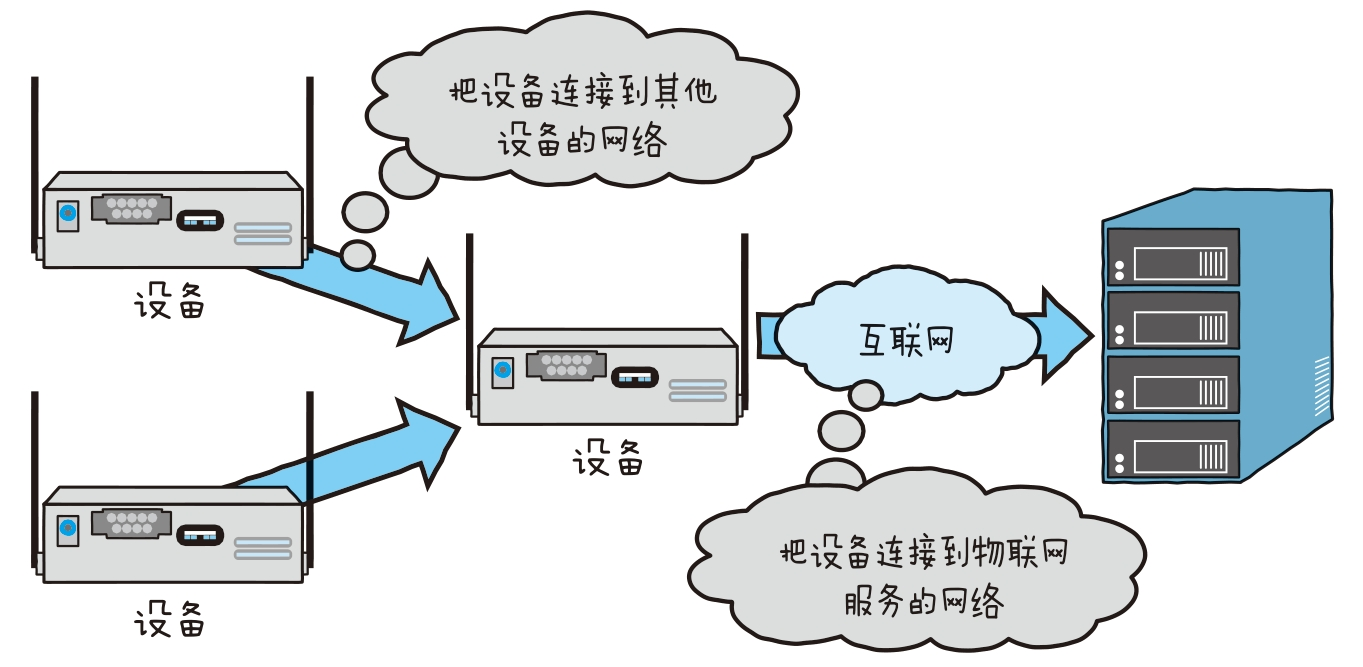
\includegraphics[width=1\linewidth]{12}
	\caption{用于物联网的两种网络}
	\label{fig:1}
\end{figure}

\subsubsection{把设备连接到其他设备的网络}

无法直接连接到互联网的设备也是存在的。我们通过把设备连接到其他设备,就能通过其他设备把这些不能连接到互联网的设备连接到互联网。前面我们介绍的传感器节点和网关正是两个典型的例子。此外,还有通过智能手机把可穿戴设备采集到的数据发送给物联网服务这一办法。

蓝牙和 ZigBee 是两种具有代表性的网络标准。它们是用无线连接的,利用的通信协议也是固定的。这些协议的特征有采用擅长近距离通信的无线连接、低功耗、易于嵌入嵌入式设备等。

要把设备连接到其他设备,除了 1 对 1 之外,还可以采用 1 对 N、N 对 N 的方式连接。特别是 N 对 N 连接的情况,我们称这种情况为网状网络(图 1.13)。

\begin{figure}[htbp]
	\centering
	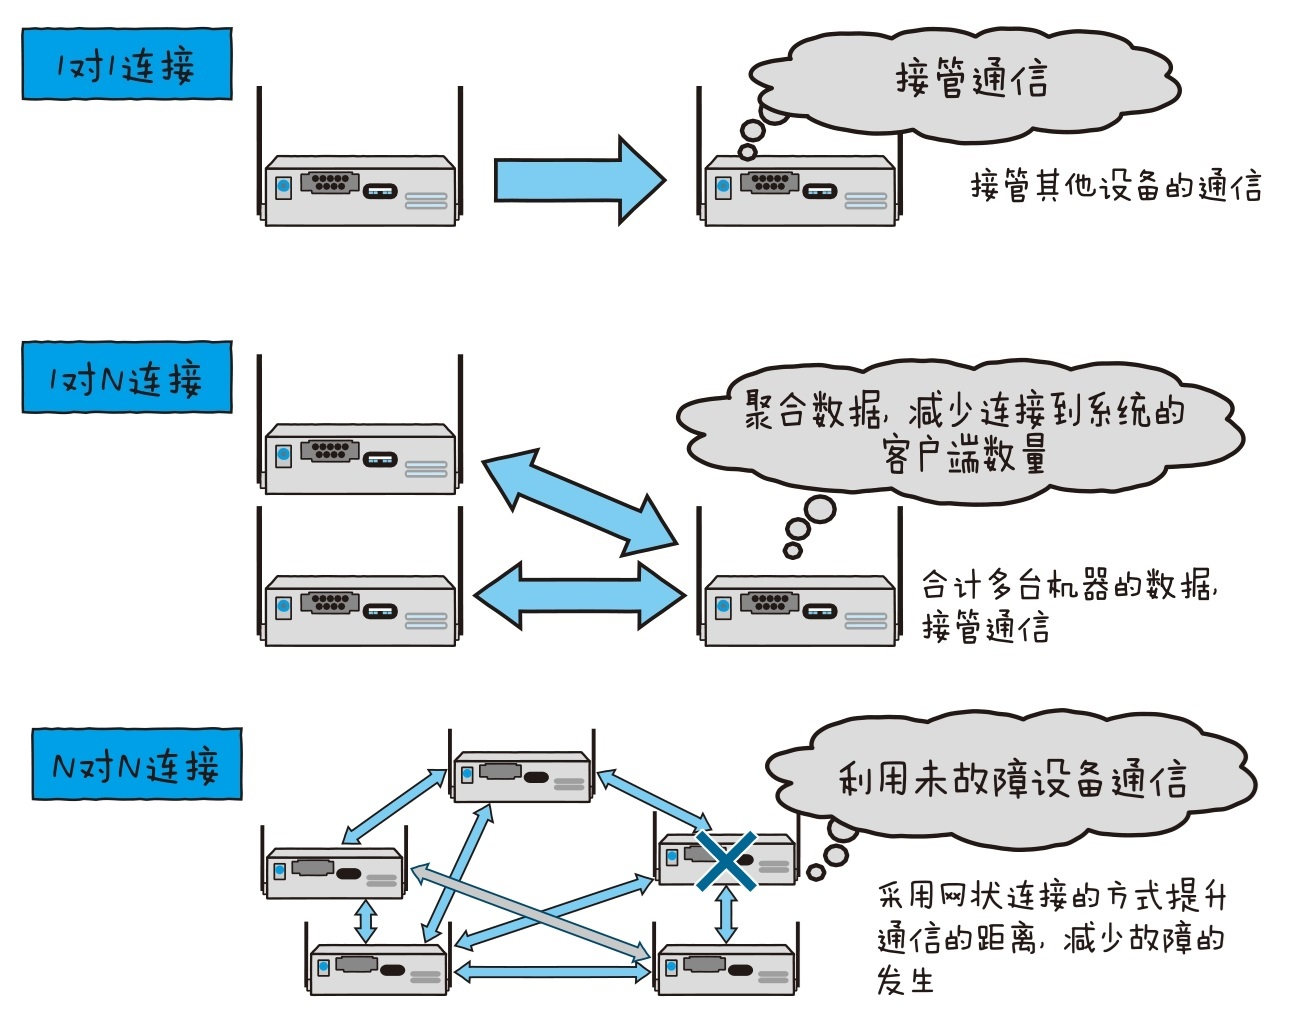
\includegraphics[width=1\linewidth]{13}
	\caption{设备之间的网络连接}
	\label{fig:1}
\end{figure}

有一种与网状网络对应的通信标准,名为 ZigBee。通过采用 N 对 N 的通信方式,设备可以一边接管其他的设备,一边进行远程通信。除此之外它还有一个优点,那就是即使有一台设备发生故障无法通信,其他设备也会代替它来执行通信。

关于上述设备的通信规格我们会在第 3 章讲解。

\subsubsection{把设备连接到服务器的网络}

把设备连接到物联网服务的网络时,会用到互联网线路。3G 和 LTE 等移动线路最为常用。

除了现在 Web 服务中广泛使用的 HTTP 和 WebSocket 协议以外,还有一些专为机器对机器通信和物联网而产生的轻量级协议,如 MQTT 等。关于该协议,我们会在第 2 章进行详细说明。

\subsection{物联网服务}

物联网服务有两个作用:一是从设备接收数据以及发送数据给设备;二是处理和保存数据(图 1.14)。

\begin{figure}[htbp]
	\centering
	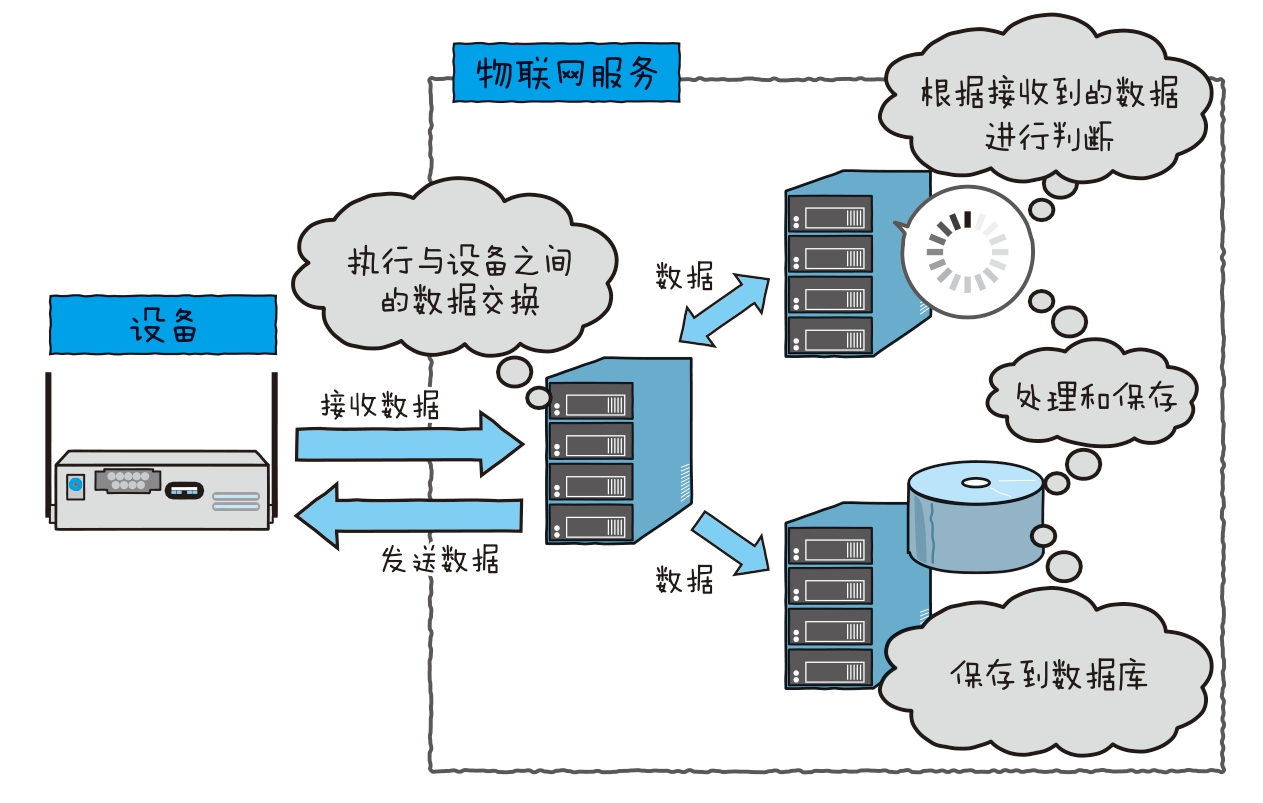
\includegraphics[width=1\linewidth]{14}
	\caption{Web 系统的作用}
	\label{fig:1}
\end{figure}

我们来具体看一下这两个作用。

\subsubsection{数据交换}

通常的 Web 服务会根据 Web 浏览器发送的 HTTP 请求发送 HTML,然后用 Web 浏览器显示。物联网服务则不采用 Web 浏览器,而是接收从设备直接发来的数据。设备发来的数据内容包括设备搭载的传感器所采集到的信息,以及用户对设备进行的操作。设备和物联网服务的通信方法大致分为两种:同步传输和异步传输(图 1.15)。

在同步传输的情况下,设备发送数据时会把数据发送给物联网服务。接下来直到物联网服务接收完数据之前,不管设备向物联网服务发送多少次数据,都算作一次传输。反过来,物联网服务在执行对设备的反馈时,则是先由设备向物联网服务发送请求消息,然后物联网服务会响应请求并将消息发送给设备。就这种方法而言,直到设备发送请求之前,物联网服务都不能把消息发送给设备。但是这种方法只适用于不知
道设备 IP 地址的情况,因为就算不知道设备的 IP 地址,只要设备发送了请求,物联网服务就能把消息发送给设备。

在异步传输中,设备会把数据发送给物联网服务,每发送一次,就算作一次传输。此外,从物联网服务向设备进行传输时,无需等待设备发来的请求,可以在任意时间点执行发送。采用这个方法能在物联网服
务规定的任意一个时刻发送消息。但是,物联网服务需要预先知道发送消息的设备的 IP 地址。

\begin{figure}[htbp]
	\centering
	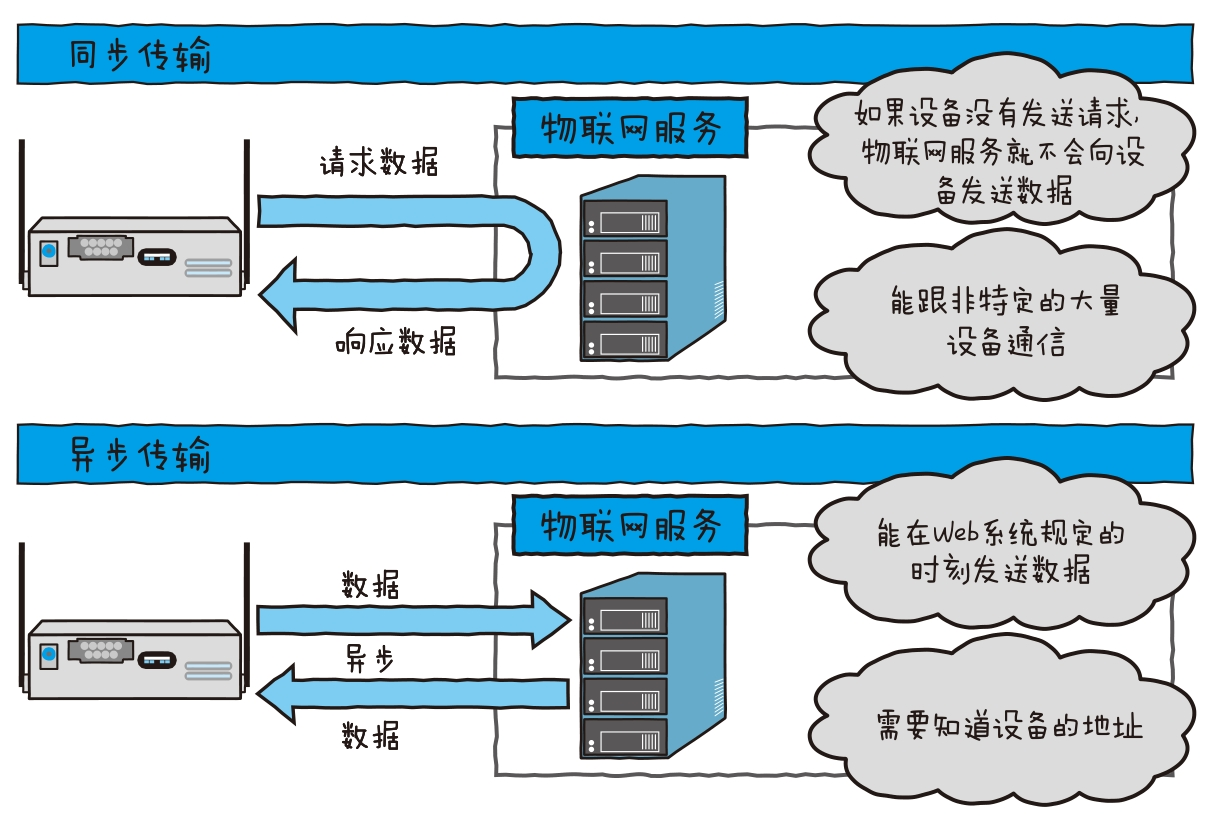
\includegraphics[width=1\linewidth]{15}
	\caption{Web 系统和设备的通信}
	\label{fig:1}
\end{figure}

第 2 章会用一些实际使用的协议来讲解这种通信。

\subsubsection{处理和保存数据}

就如大家在图 1.14 看到的那样,处理和保存数据的操作包括把从设备接收到的数据保存到数据库,以及从接收到的数据来判断如何控制设备。

从设备接收到的数据不只有能用计算机简单处理的数值型数据,根据要实现的内容,还包含图像、语音、自然语言这些很难直接用计算机处理、没有被结构化的数据。我们把这种数据叫作非结构化数据。处理
时,有时也会把那些易于用计算机处理的数据从非结构化数据中提取出来,例如把表示图像和语音特征的值提取出来。这些信息会被保存到数据库中。

设备按照所提取数据的判断逻辑来决定反馈的内容,例如基于某个房间的温度数据来决定空调的开关状态和目标温度。这些处理和保存的方法大体上分为两种:一种是对保存的数据定期进行采集和处理的批处
理,另一种是将收到的数据逐次进行处理的流处理(图 1.16)。

\begin{figure}[htbp]
	\centering
	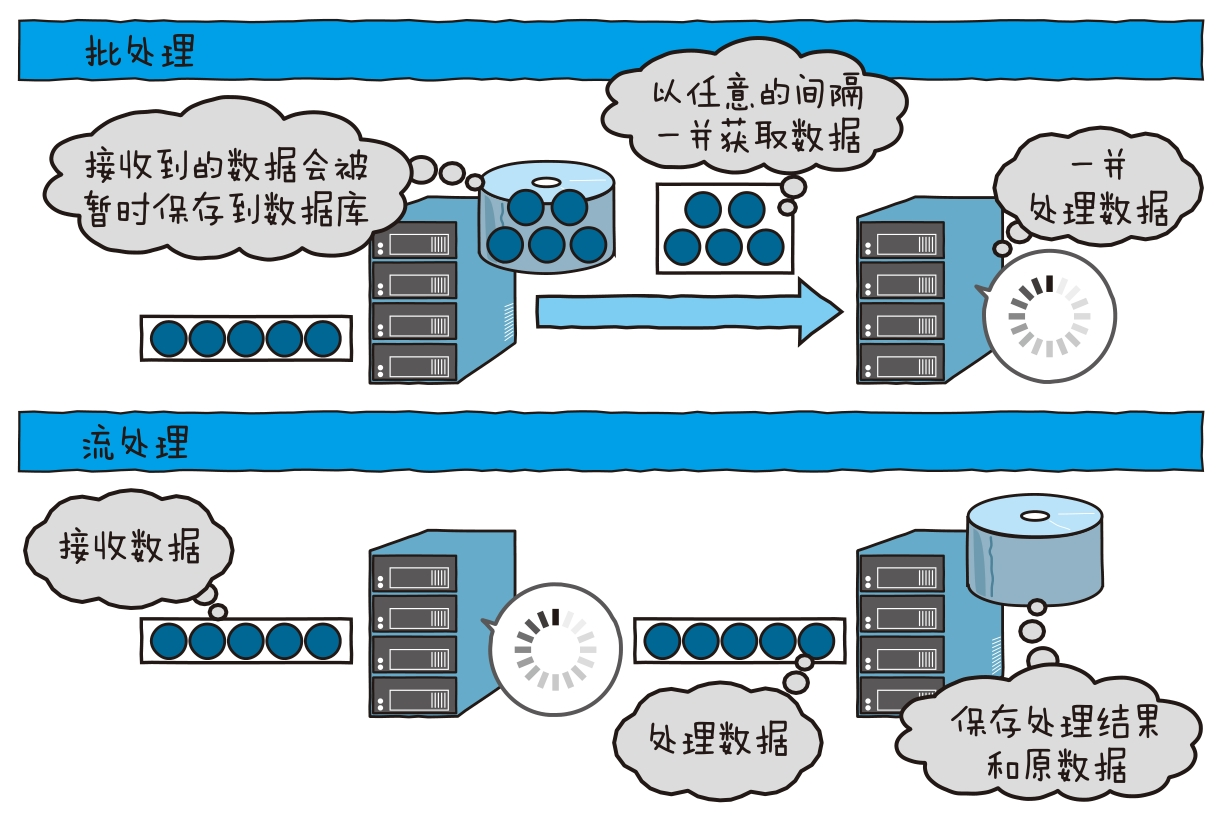
\includegraphics[width=1\linewidth]{16}
	\caption{保存和处理数据的时机}
	\label{fig:1}
\end{figure}

根据房间的温度变化来调整空调的运转时,从向空调发出指示到温度发生变化,这中间会需要一段时间。这种情况下就适合采用批处理来持续记录每隔一定时间的温度值,并定期执行处理。此外,如果希望回到房间之后再打开空调,那么就适合采用能立即执行操作的流处理。

\subsection{数据分析}

前一节我们以“温度传感器和空调运转的关系”为例进行了说明。那么我们能像这个例子那样,轻松实现“根据房间温度控制空调”这一目的吗?

要实现这一目的,需要决定控制空调开 / 关的房间温度值,也就是决定温度的阈值。这种情况下,阈值会根据使用者目的而有所不同。举个例子,把空调的功耗降到最小所需要的阈值和保持令人体感舒适的温
度所需要的阈值就是两个不同的值。此外,为了能准确判断房间里有没有人,需要从多个传感器的值所包含的关联性来判断人在或不在房间里。人类很难光凭经验去摸索和决定这种值。这就凸显出了数据分析的
重要性。

数据分析的代表性方法有两种,分别是统计分析和机器学习。这里就来看看我们用这两种方法能办到什么(图 1.17)。

\begin{figure}[htbp]
	\centering
	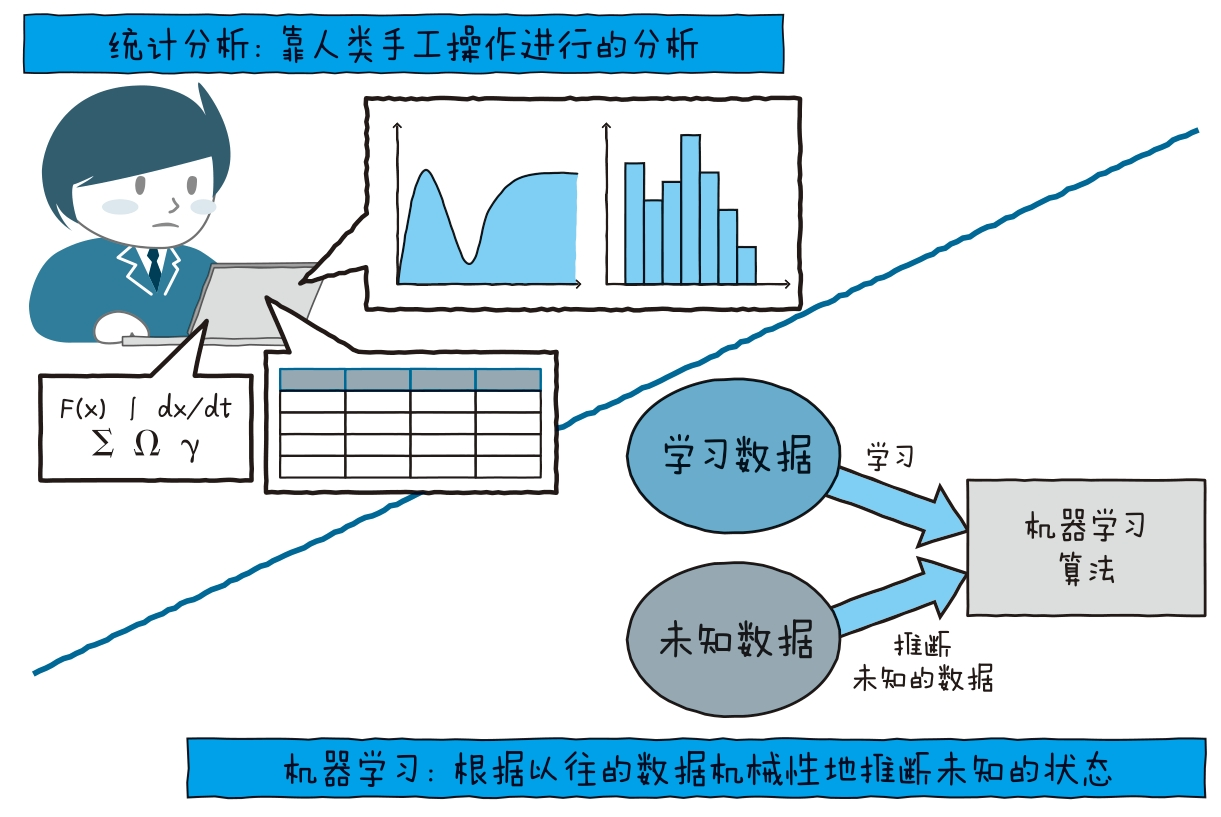
\includegraphics[width=1\linewidth]{17}
	\caption{数据分析的两种方法}
	\label{fig:1}
\end{figure}

\subsubsection{统计分析}

统计分析是用数学手法通过搜集到的大量数据来明确事物的联系性的方法。比如为了实现给空调节能的目的,我们调查了空调在某个固定的温度下运转时,房间的温度和空调的耗电量,并将这些数据制成了表格(图 1.18)。

\begin{figure}[htbp]
	\centering
	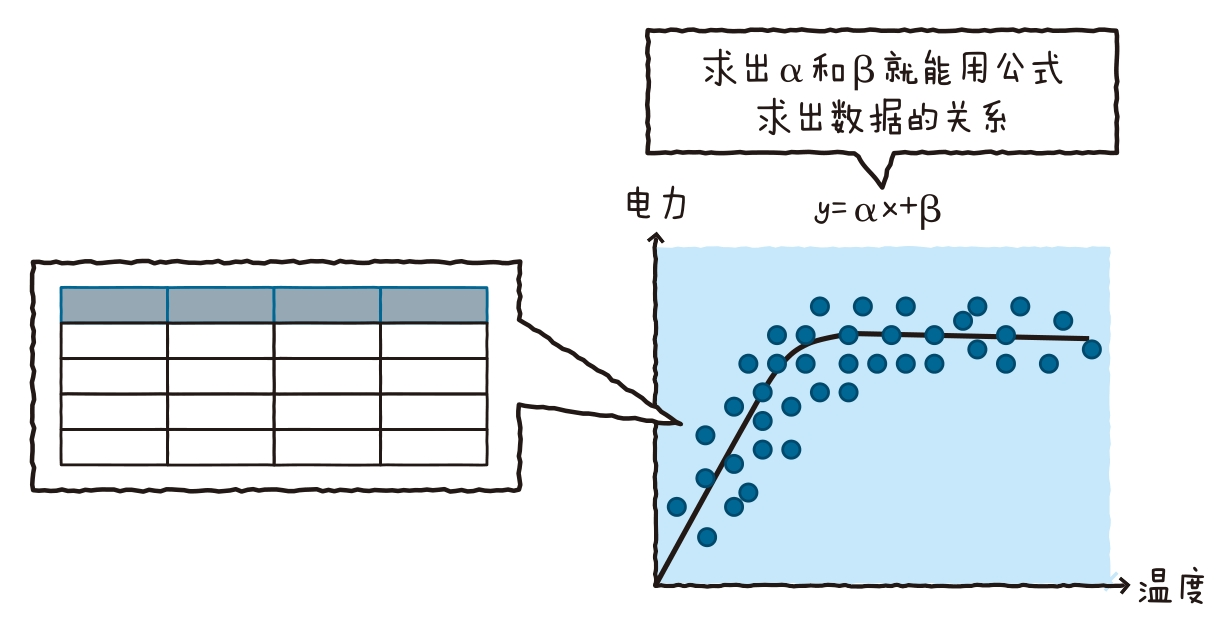
\includegraphics[width=1\linewidth]{18}
	\caption{空调的电力和室温的关系示例}
	\label{fig:1}
\end{figure}

从这个关系中可以推导出在室温下把空调温度设定在多少才能最省电,由此就能决定阈值了。

上述示例采用的是先填表再分析的方法,除此之外还有一种叫作回归分析的统计方法,此方法我们会在第 6 章详细说明。

\subsubsection{机器学习}

统计分析基于大量数据之间的联系性,明确当前数据间形成的关联。机器学习则不仅仅能进行分析,还能预测今后的发展状况。

机器学习就如它的字面意思一样,计算机会按照程序决定的算法,机械性地学习所给数据之间的联系性。当给出未知数据时,也会输出与其对应的值。

机器学习分为两个阶段:学习阶段和识别阶段(图 1.19)。在学习阶段,一个名为学习器的程序会基于一些训练数据,机械性地掌握这些数据之间的联系。作为学习阶段的结果,计算机会根据机器学习的算法输出参数,然后以这个参数为基础创建叫作鉴别器(discriminator)的程序。只要把未知的数据给这个鉴别器,就能输出最适合这个值的结果。

\begin{figure}[htbp]
	\centering
	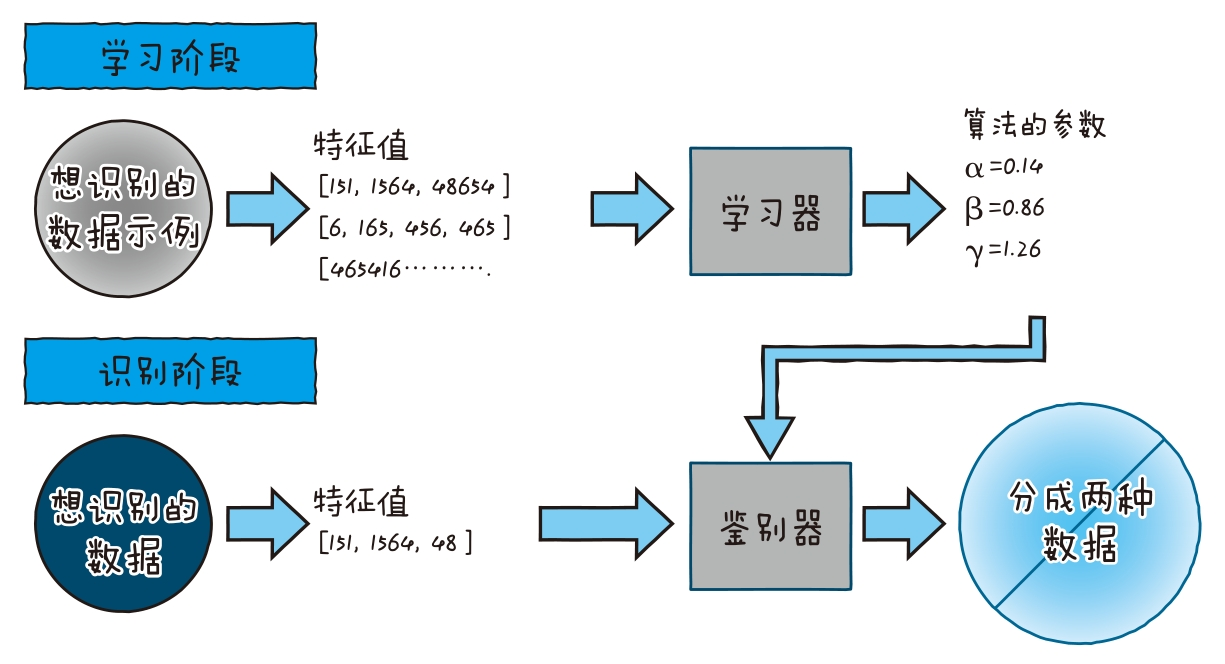
\includegraphics[width=1\linewidth]{19}
	\caption{机器学习示例}
	\label{fig:1}
\end{figure}

举个例子,假设我们想使用若干种传感器来识别房间里有没有人。这种情况下需要准备两种数据,即房间里有人时的传感器数据(正面例子)和房间里没人时的传感器数据(反面例子)。计算机通过把这两种数据分别交给学习器,可以获取制作鉴别器用的参数。对于以参数为基准制作的鉴别器而言,只要输入从各个感测设备接收到的数据,鉴别器就能输出结果,告诉我们现在房间里是否有人。

上述内容属于机器学习的示例之一,被称作分类问题。在用于执行数据分类的机器学习算法中有很多途径,如用于垃圾邮件过滤器的贝叶斯过滤器和用于分类文档及图像的支持向量机(Support Vector Machine,SVM)等。此外,除了分类问题以外,机器学习还能解决很多领域的问题。

\chapter{物联网的架构}

\section{物联网的整体结构}

实现物联网时,物联网服务大体上发挥着两个作用。

第一是把从设备收到的数据保存到数据库,并对采集的数据进行分析。

第二是向设备发送指令和信息。

本章将会为大家介绍如何构建物联网服务,以及用于实现物联网的重要要素。

\subsection{整体结构}

物联网大体上有 3 个构成要素,如图 2.1 所示。一个是设备,另一个是网关,再来就是服务器。关于设备的基本结构和使用的技术,我们会在第 3 章详细说明。因此本章并不涉及设备。我们来详细看一下用怎样的机制才能实现网关和服务器。

\begin{figure}[htbp]
	\centering
	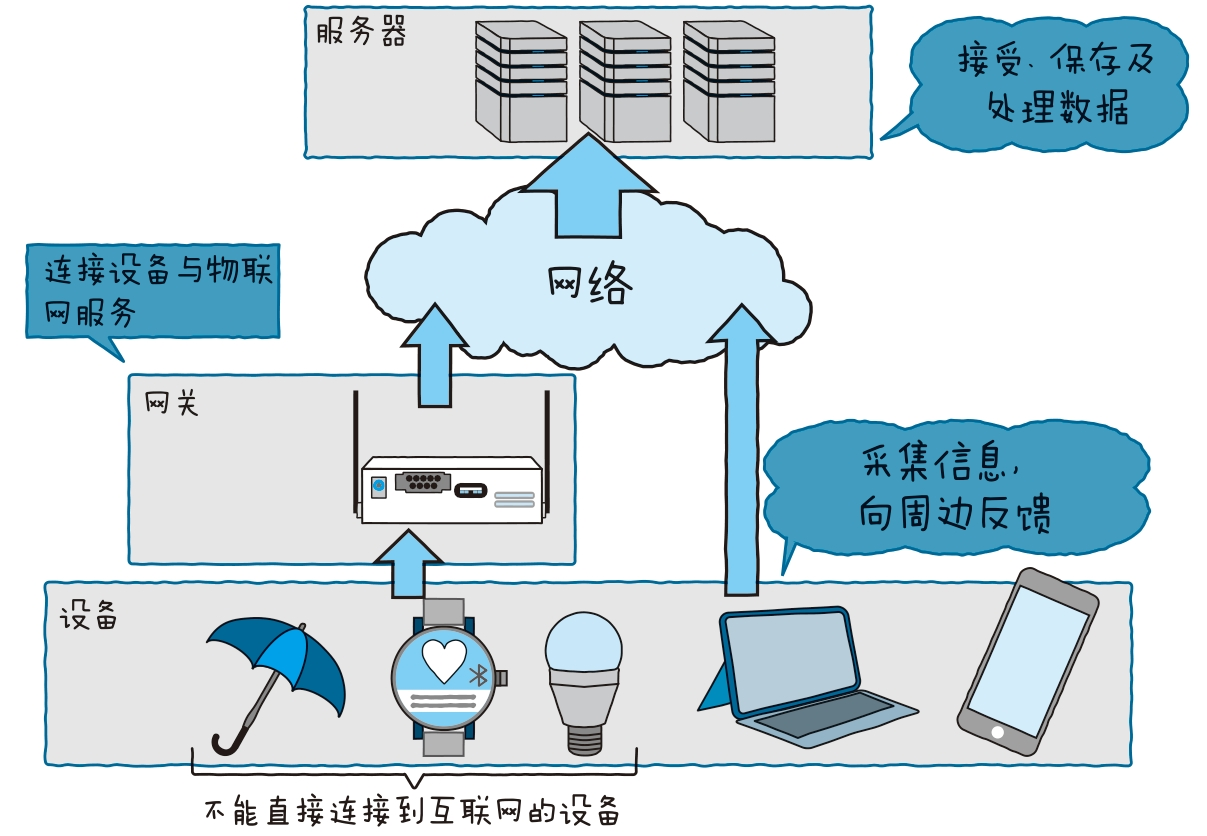
\includegraphics[width=1\linewidth]{20}
	\caption{物联网的整体结构}
	\label{fig:1}
\end{figure}

\subsection{网关}

如图 2.1 左下所示,物联网使用的设备中,有 3 台设备不能直接连接到互联网。网关就负责把这些设备转发到互联网。

网关指的是能连接多台设备,并具备直接连接到互联网的功能的机器和软件(图 2.2)。如今,市面上有很多种网关。在多数情况下,网关凭借 Linux 操作系统来运行。

\begin{figure}[htbp]
	\centering
	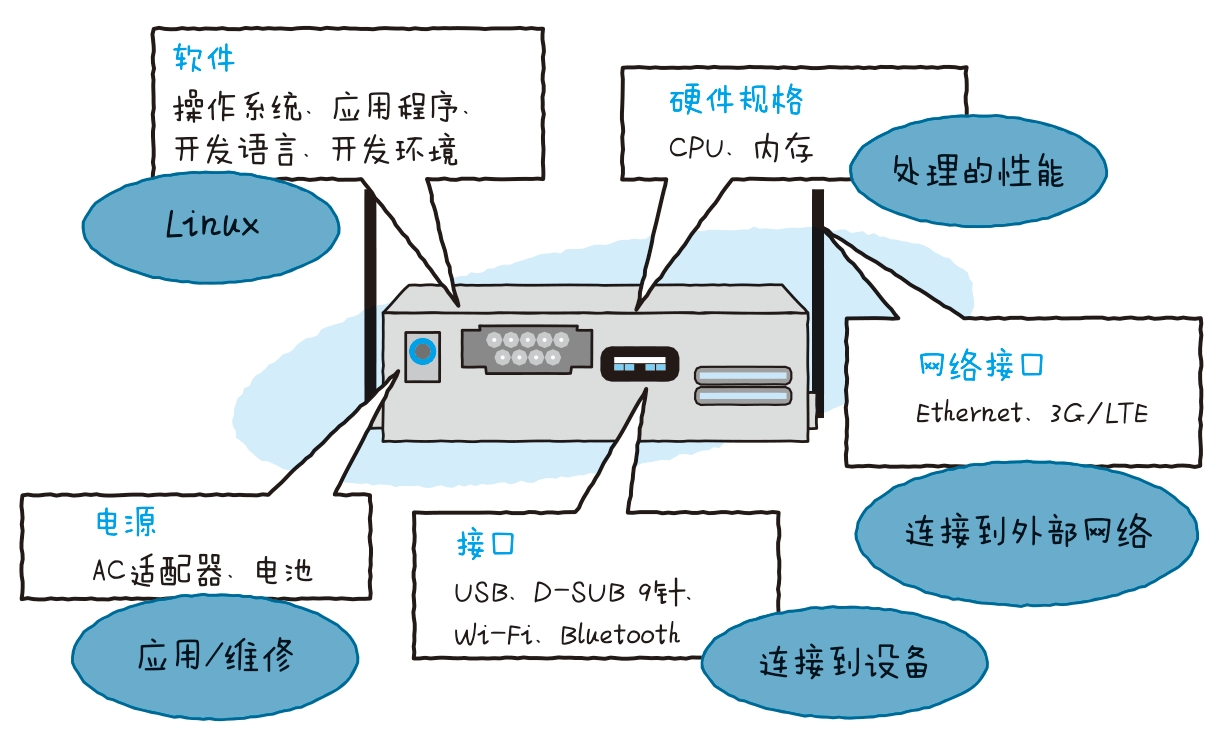
\includegraphics[width=1\linewidth]{21}
	\caption{选择网关的标准}
	\label{fig:1}
\end{figure}

选择网关时有几项重要的标准,我们来一起看一下。

\subsubsection{接口}

第一重要的是用于连接网关和设备的接口。网关的接口决定了能连接的设备,因此重点在于选择一个适配设备的接口。

有线连接方式包括串行通信和 USB 连接。串行通信中经常用的是一种叫作 D-SUB 9 针(pin)的连接器,而 USB 连接中用到的 USB 连接器则种类繁多。

无线连接中用的接口是蓝牙和 Wi-Fi(IEEE 802.11)。此外,还有采用 920 MHz 频段的 Zigbee 标准,以及各制造商们的专属协议。第 3 章会详细讲解这些规格各自的特征,重点在于根据设备对应的标准来选择接口。

\subsubsection{网络接口}

我们用以太网或是 Wi-Fi、3G/LTE 来连接外部网络。网络接口会影响到网关的设置场所。以太网采用有线连接,通信环境稳定。然而正因为采用的是有线连接,所以必须把 LAN 电缆布线到网关的设置场所。因此,在设置场所方面就会在某种程度上受到限制。

对 3G/LTE 连接而言,设置场所就比较自由了,但通信的质量会受信号强弱影响,所以通信不如有线连接稳定。因此,有时很难在信号不良的大楼和工厂等封闭环境中设置。不过,3G/LTE 连接有个好处,即
只使用网关就能完成和外部的通信,因此操作起来很简单。此外,想使用 3G/LTE 时,需要和电信运营商签订协议并获取 SIM 卡,这点就跟使用手机一样。

\subsubsection{硬件}

相对于一般计算机而言,网关在 CPU 和内存这些硬件的性能方面比较受限。我们需要确定让网关做哪些事情,也需要考虑到它的硬件性能。

\subsubsection{软件}

人们主要使用 Linux 操作系统来运行网关。虽然有很多种用于服务器的 Linux,不过,网关上搭载的 Linux 是面向嵌入式的。

此外,还有一个叫作 BusyBox 的软件,它运行起来占用内存少,集成了标准的 Linux 命令工具。它用于在硬件资源匮乏的时候运行网关。除此之外,还要考虑是否有用于控制网关功能的程序库,以及与这种程序库对应的语言等。

\subsubsection{电源}

说起来,电源很容易被人们遗忘。网关基本上都是使用 AC 适配器当电源的,因此需要事先在设置网关的场所准备好电源。如果网关本身搭载有电池,那么就不需要准备电源了,不过需要进行充电等维护工作。

\subsection{服务器的结构}

在功能方面,物联网服务大体上可分为 3 个部分,本书分别称它们为前端部分、处理部分,以及数据库部分(图 2.3)。

\begin{figure}[htbp]
	\centering
	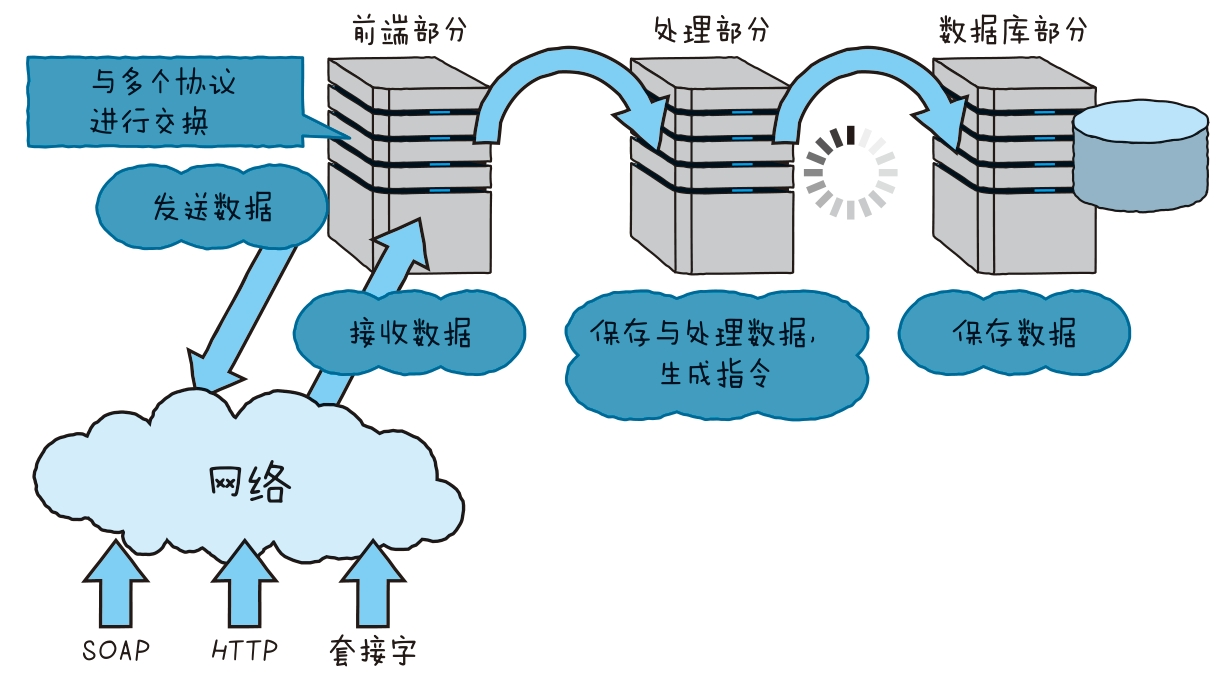
\includegraphics[width=1\linewidth]{22}
	\caption{物联网服务的 3 个功能}
	\label{fig:1}
\end{figure}

首先,前端部分包括数据接收服务器和数据发送服务器。数据接收服务器接收设备和网关发来的数据,转交给后续的处理部分。数据发送服务器则刚好相反,它负责把从处理服务器接收到的内容发送给设备。

通常情况下,Web 服务的前端部分只接受 HTTP 协议。而物联网服务的前端部分则需要根据连接设备的不同来匹配 HTTP 以外的协议。使用者需要考虑到协议的实时性和通信的轻量化,以及能否以服务器为起
点发送数据。我们会在 2.2 节重新讲解这些协议。

处理部分负责处理从前端部分接收到的数据。这里的“处理”指的是分解数据、存储数据、分析数据、生成发给设备的通知内容,等等。数据处理包括批处理和流处理等,批处理即把数据存入数据库之后一并进行处理,而流处理是逐次处理从前端部分收到的数据。使用者需要根据处理内容和数据特性来灵活使用这些“处理”。

最后是数据库。这里的数据库不只会用到关系数据库,还会用到 NoSQL 数据库。当然,使用者需要根据想存储的数据和想使用的方法来选择数据库。

\section{采集数据}

\subsection{网关的作用}

就如我们前面说的那样,网关是一台用于把不能直接连接到互联网的设备转发连接到互联网的设备。再往细了说,网关是由 3 种功能构成的(图 2.4)。

\begin{figure}[htbp]
	\centering
	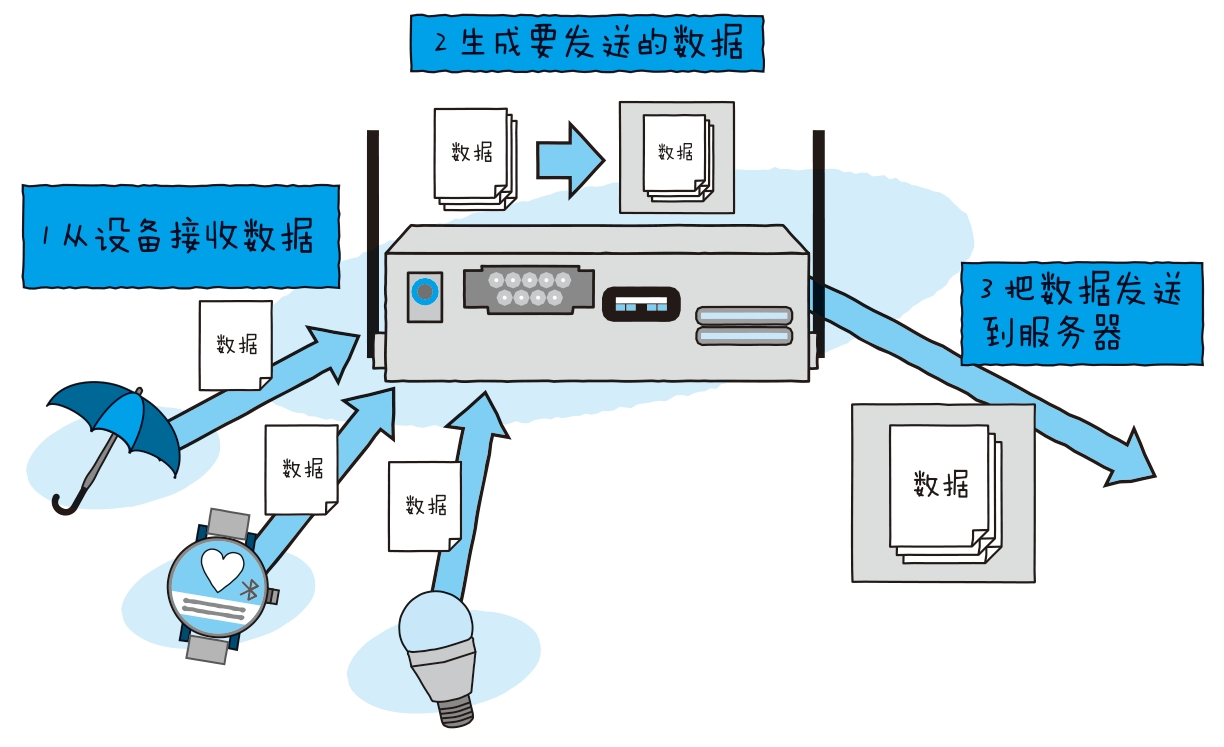
\includegraphics[width=1\linewidth]{23}
	\caption{网关的功能}
	\label{fig:1}
\end{figure}

这 3 种功能分别是连接设备功能、数据处理功能和向服务器发送数据的功能。此外,实际使用网关执行应用时,还需要其他的管理应用功能。管理应用功能会在第 5 章单独介绍。

接下来就来详细看看网关的 3 种功能。

\subsubsection{连接设备}

设备和网关是通过各种各样的接口连接的。当通过传感器终端连接时,多数情况下是传感器单方面持续向服务器发送数据。根据设备不同,也存在设备申请从外部获取数据时,服务器向设备发送数据的情况,这时就需要通过网关申请数据。

\subsubsection{生成要发送的数据}

接下来把从设备接收到的数据转化成能发送给服务器的格式。在表示从设备发送到网关的数据时,也有把 4 位二进制数(如二进制数据和 BCD 码)替换成一位十进制数数据来表示的(图 2.5)。这样的数据不会被直接发给服务器,而是在网关处被转化成数值数据和字符串的格式。

\begin{figure}[htbp]
	\centering
	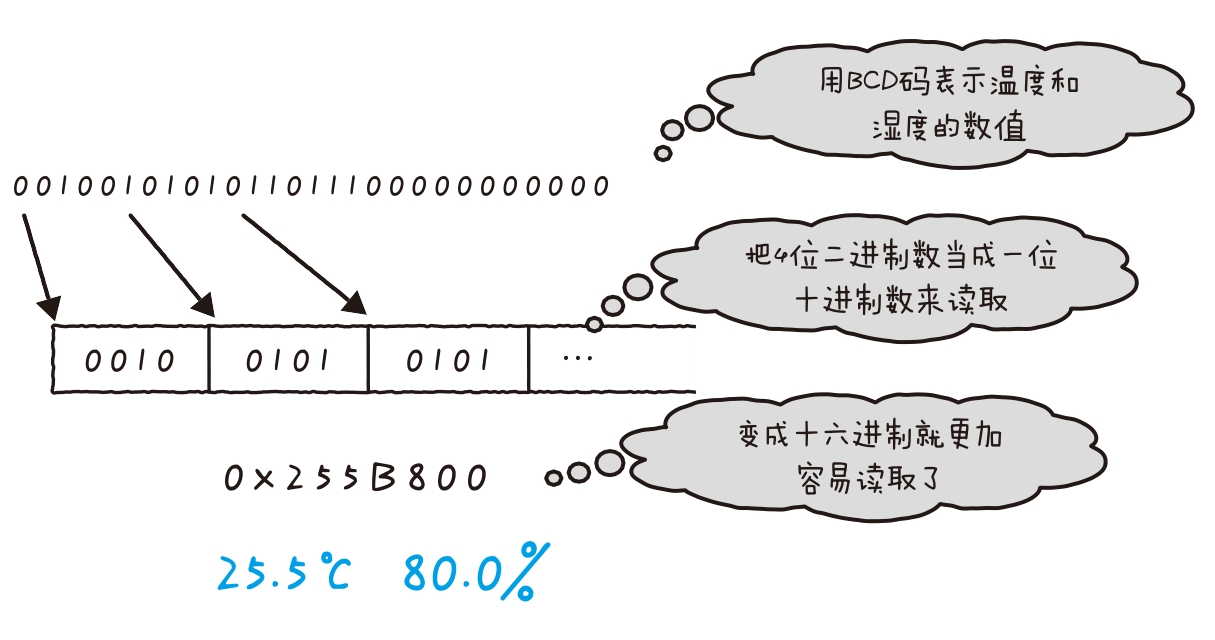
\includegraphics[width=1\linewidth]{24}
	\caption{BCD 码}
	\label{fig:1}
\end{figure}

还存在下面这种情况:不把每台设备发来的数据直接发送给服务器,而是将大量数据整合在一起再发送给服务器。这么做有以下两个原因。

第一,通过整合数据能减少数据的附加信息,减少数据量。第二,通过一并发送数据能减轻访问物联网服务时对服务器造成的负担。

\subsubsection{发送数据给服务器}

向物联网服务发送数据。此时,需要根据服务器来决定发送数据的时间间隔和发送数据的协议。另外,为了能从物联网的服务器接收消息,还得事先准备好这种功能。

\section{接收数据}

\subsection{数据接收服务器的作用}

数据接收服务器就跟它的字面意思一样,负责接收从设备发送来的数据。它在设备和系统之间起着桥梁作用。有很多种方法可以从设备把数据发送给服务器,其中具有代表性的包括以下两种方法。

● 准备一个使用了 HTTP 协议的 Web API 来访问设备(如通常的 Web 系统)

● 执行语音和视频的实时通信(如 WebSocket 和 WebRTC)

除此之外,还出现了一种名为 MQTT 的、专门针对物联网的新型通信协议。

本章将为大家介绍 HTTP 协议、WebSocket、MQTT 这几个典型协议。

\subsection{HTTP 协议}

HTTP 协议提供的是最大众化且最简易的方法。使用一般的 Web 框架就可以制作数据接收服务器。设备用 HTTP 的 GET 方法和 POST 方法访问服务器,把数据存入请求参数和 BODY 并发送(图 2.6)。

\begin{figure}[htbp]
	\centering
	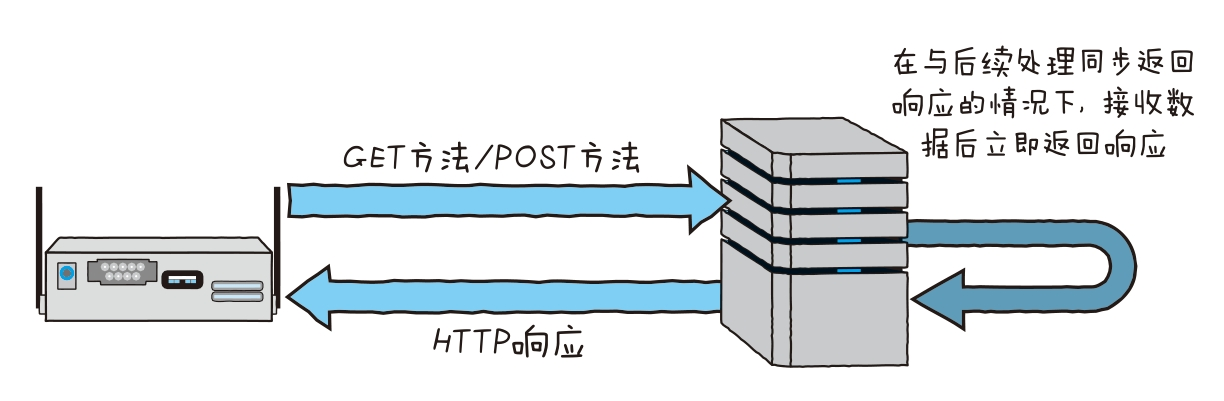
\includegraphics[width=1\linewidth]{25}
	\caption{通过 HTTP 协议发送和接收数据}
	\label{fig:1}
\end{figure}

HTTP 协议是 Web 的标准协议,这一点自不用说。因此 HTTP 协议和 Web 的兼容性非常强。此外,因为 HTTP 协议有非常多的技术诀窍,所以我们必须在制作实际系统时审视服务器的结构,应用程序的架构以及安全性等。关于这点,有很多事例值得参考。另外,HTTP 协议还准备了 OSS 的框架,方便人们使用。

\subsubsection{REST API}

设备应该如何访问物联网服务呢?用 HTTP 协议访问的时候,也得从 GET 和 POST 中选择一种合适的方法来访问。除了物联网服务,一般 Web 服务中公开的 API 也应格外重视这个问题。

在 Web 服务的世界里,有一种思路叫作 RESTful。REST 是一种接口,它为特定的 URL 指定参数并执行访问,作为其响应来获取结果。它通过用多个 HTTP 方法访问一个 URL,来对一个 URL 执行获取和注册数据。这样一来,URL 的作用就易于理解了。

例如,使用 GET 方法访问 /sensor/temperature 就能获取温度传感器的值。使用 POST 方法一并访问传感器数据,就会追加新的传感器数据。

如果想用除了 RESTful 以外的方法实现同样的功能,就需要生成用于获取以往数据的 URL 和追加数据的 URL,并决定其分别用 GET 方法访问还是用 POST 方法访问。RESTful 的思路保证了 URL 设计的简单性,请大家务必审视一下 RESTful 的思路。

\subsection{WebSocket}

WebSocket 是一种通信协议,用于在互联网上实现套接字通信。它实现了 Web 浏览器和 Web 服务器间的数据双向连续传输。

就 HTTP 协议而言,每次发送数据都必须生成发送数据用的通信路径及连接。此外,一般情况下,客户端没有发出申请就不能进行通信。

相对而言,WebSocket 就不同了。只要一开始根据客户端发出的连接申请确立了连接,就能持续用同一个连接传输数据。另外,只要确立了连接,就算客户端没有发出申请,服务器也能给客户端发送数据(图
2.7)。

\begin{figure}[htbp]
	\centering
	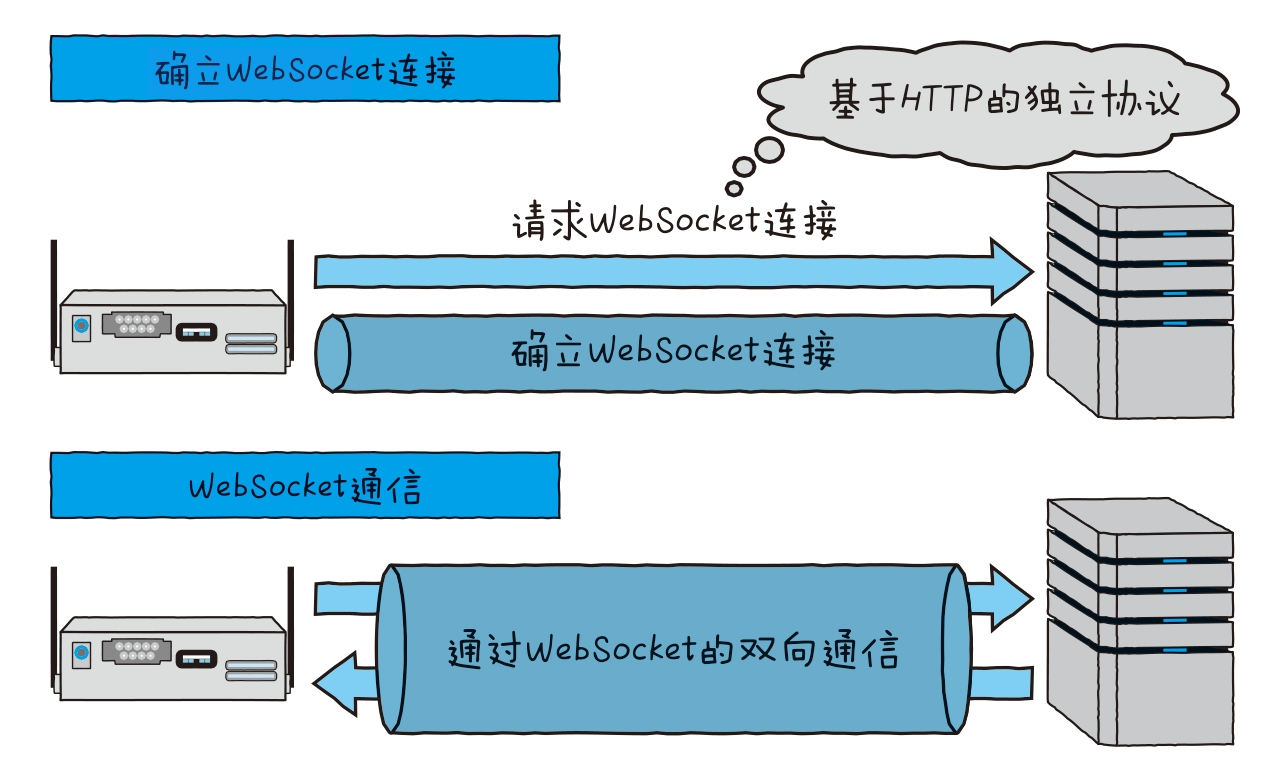
\includegraphics[width=1\linewidth]{26}
	\caption{通过 WebSocket 协议传输数据}
	\label{fig:1}
\end{figure}

这样一来,在发送语音数据等连续的数据,以及发生与服务器的相互交换时,就能使用 WebSocket 了。WebSocket 自身只提供服务器与客户端的数据交换,因此需要使用者另外决定在应用层上使用的协议。

\subsection{MQTT}

MQTT(MQ Telemetry Transport,消息队列遥测传输)是近年来出现的一种新型协议,物联网领域会将其作为标准协议。MQTT 原本是 IBM 公司开发的协议,现在则开源了,被人们不断开发着。

MQTT 是一种能实现一对多通信(人们称之为发布或订阅型)的协议。它由 3 种功能构成,分别是中介(broker)、发布者(publisher)和订阅者(subscriber)(图 2.8)。

\begin{figure}[htbp]
	\centering
	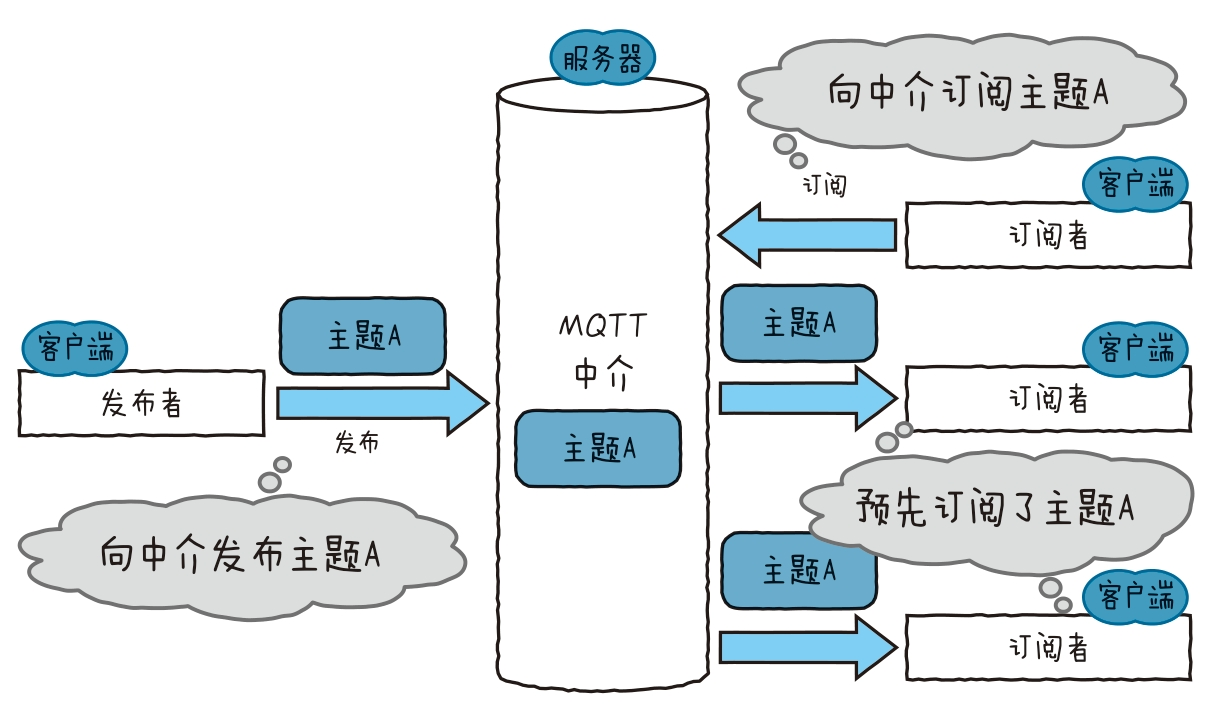
\includegraphics[width=1\linewidth]{27}
	\caption{通过 MQTT 传输消息}
	\label{fig:1}
\end{figure}

中介承担着转发 MQTT 通信的服务器的作用。相对而言,发布者和订阅者则起着客户端的作用。发布者是负责发送消息的客户端,而订阅者是负责接收消息的客户端。MQTT 交换的消息都附带“主题”地址,各个客户端把这个“主题”视为收信地址,对其执行传输消息的操作。形象地比喻一下,中介就是接收邮件的邮箱。

再来详细看一下 MQTT 通信的机制(图 2.9)。首先,中介在等待各个客户端对其进行连接。订阅者连接中介,把自己想订阅的主题名称告诉中介。这就叫作订阅。

\begin{figure}[htbp]
	\centering
	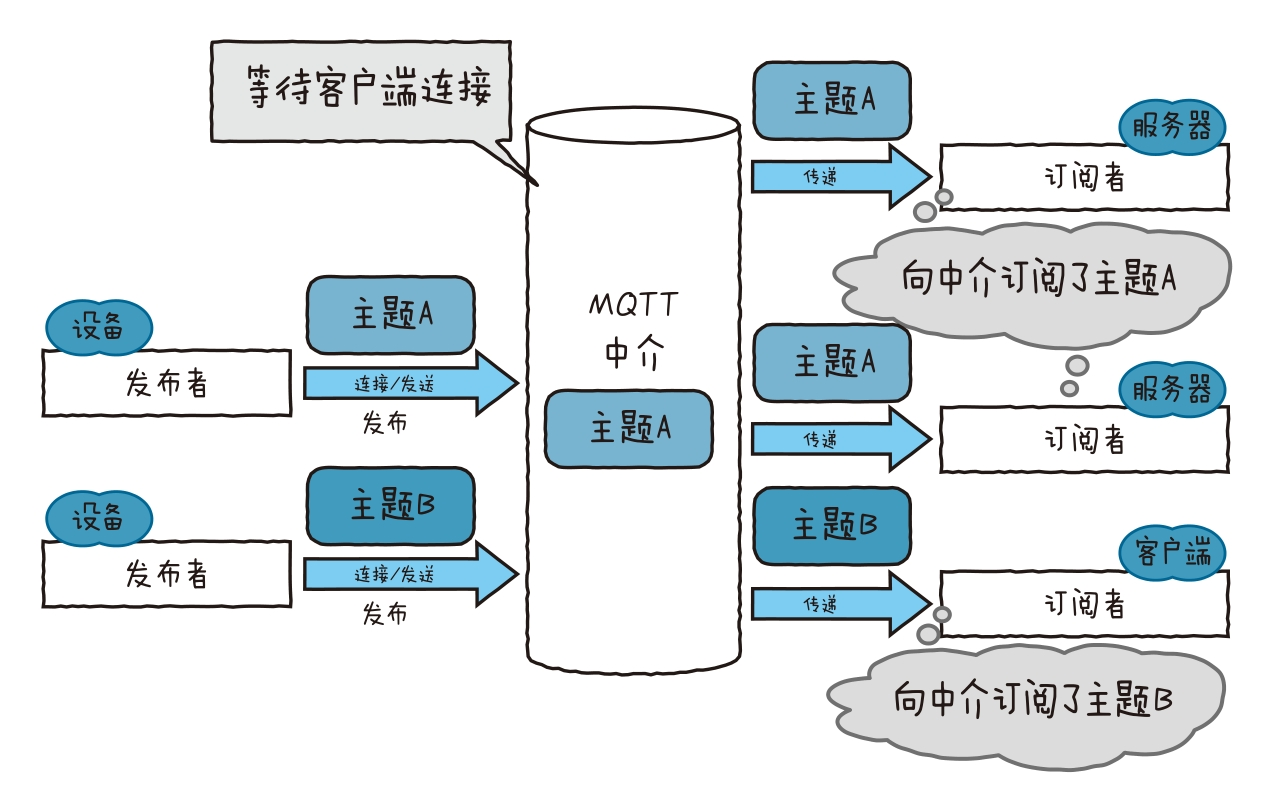
\includegraphics[width=1\linewidth]{28}
	\caption{MQTT 通信的机制}
	\label{fig:1}
\end{figure}

然后发布者连接中介,以主题为收信地址发送消息。这就是发布。

发布者一发布主题,中介就会把消息传递给订阅了该主题的订阅者。如图 2.9 所示,如果订阅者订阅了主题 A,那么只有在发布者发布了主题 A 的情况下,中介才会把消息传递给订阅者。订阅者和中介总是处于连接状态,而发布者则只需在发布时建立连接,不过要在短期内数次发布时,就需要保持连接状态了。因为中介起着转发消息的作用,所以各个客户端彼此之间没有必要知道对方的 IP 地址等网络上的收信地址。

又因为多个客户端可以订阅同一个主题,所以发布者和订阅者是一对多的关系。在设备和服务器的通信中,设备相当于发布者,服务器则相当于订阅者。

主题采用的是分层结构。用“\#”和“+”这样的符号能指定多个主题。如图 2.10 所示,/Sensor/temperature/\# 中使用了“\#”符号,这样就能指定所有开头为 /Sensor/temperature/ 的主题。此外,/Sensor/+/room1 中使用了符号“+”,这样一来就能指定所有开头是 /Sensor/、结尾是 /room1 的主题。

\begin{figure}[htbp]
	\centering
	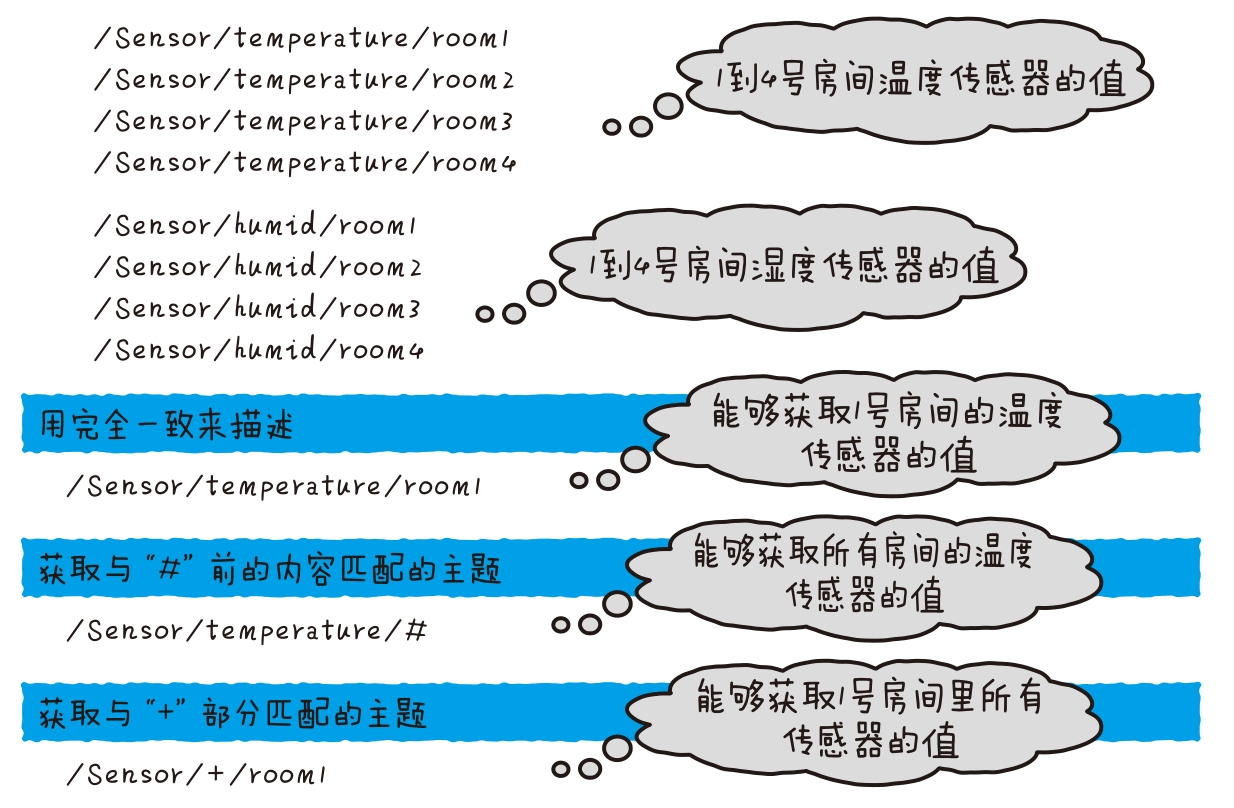
\includegraphics[width=1\linewidth]{29}
	\caption{MQTT 的主题示例}
	\label{fig:1}
\end{figure}

像这样借助于中介的发布 / 订阅型通信,MQTT 就能实现物联网服务与多台设备之间的通信。另外,MQTT 还实现了轻量型协议。因此它还能在网络带宽低、可靠性低的环境下运行;又因为消息小、协议机制简单,所以在硬件资源(设备、CPU 和内存等)受限的条件下也能运行,可以说是为物联网量身定做的协议。MQTT 本身还具备特殊的机制,下面我们会对其逐一说明。

\subsubsection{QoS}

QoS\footnote{Quality of Service	服务质量,指一个网络能够使用各种基础技术,为指定的网络	通信提供更好的服务能力,是网络的一种安全机制,也是用来解决网络延迟和阻塞等问题的一种技术。} 是 Quality of Service(服务质量)的简称。这个词在网络领域表示的是通信线路的品质保证。MQTT 里存在 3 个等级的 QoS。“发布者和中介之间”以及“中介和订阅者之间”都分别定义了不同的 QoS 等级,以异步的方式运行。此外,当“中介与订阅者之间”指定的 QoS 小于“发布者和中介之间”交换的 QoS 时,“中介与订阅者之间”的 QoS 会被降级到指定的 QoS。QoS 0 指的是最多发送一次消息(at most once)(图 2.11),发送要遵循 TCP/IP 通信的“尽力服务”\footnote{Best Effort 尽力服务,标准的因特网服务模式。在网络接口发生拥塞时,不顾及用户或应用,马上丢弃数据包,直到业务量有所减少为止。}。消息分两种情况,即到达了一次中介处,或没有到达中介处。

\begin{figure}[htbp]
	\centering
	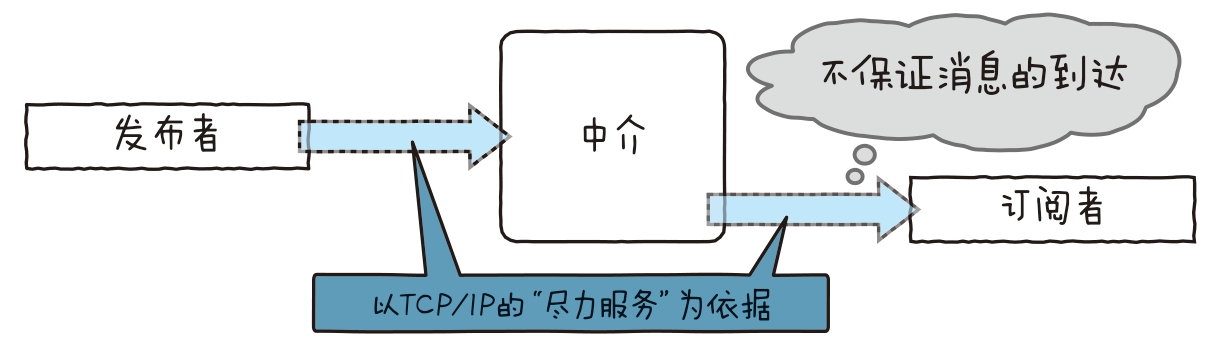
\includegraphics[width=1\linewidth]{30}
	\caption{QoS 0(最多只能发送一次)}
	\label{fig:1}
\end{figure}

接下来的 QoS 1 是至少发送一次消息(at least once)(图 2.12)。

中介一接收到消息就会向发布者发送一个叫作“PUBACK 消息”的响应,除此之外还会根据订阅者指定的 QoS 发送消息。当发生故障,或经过一定时间后仍没能确认 PUBACK 消息时,发布者会重新发送消息。
如果中介接收了发布者发来的消息却没有返回 PUBACK,那么中介会重复收到消息。

\begin{figure}[htbp]
	\centering
	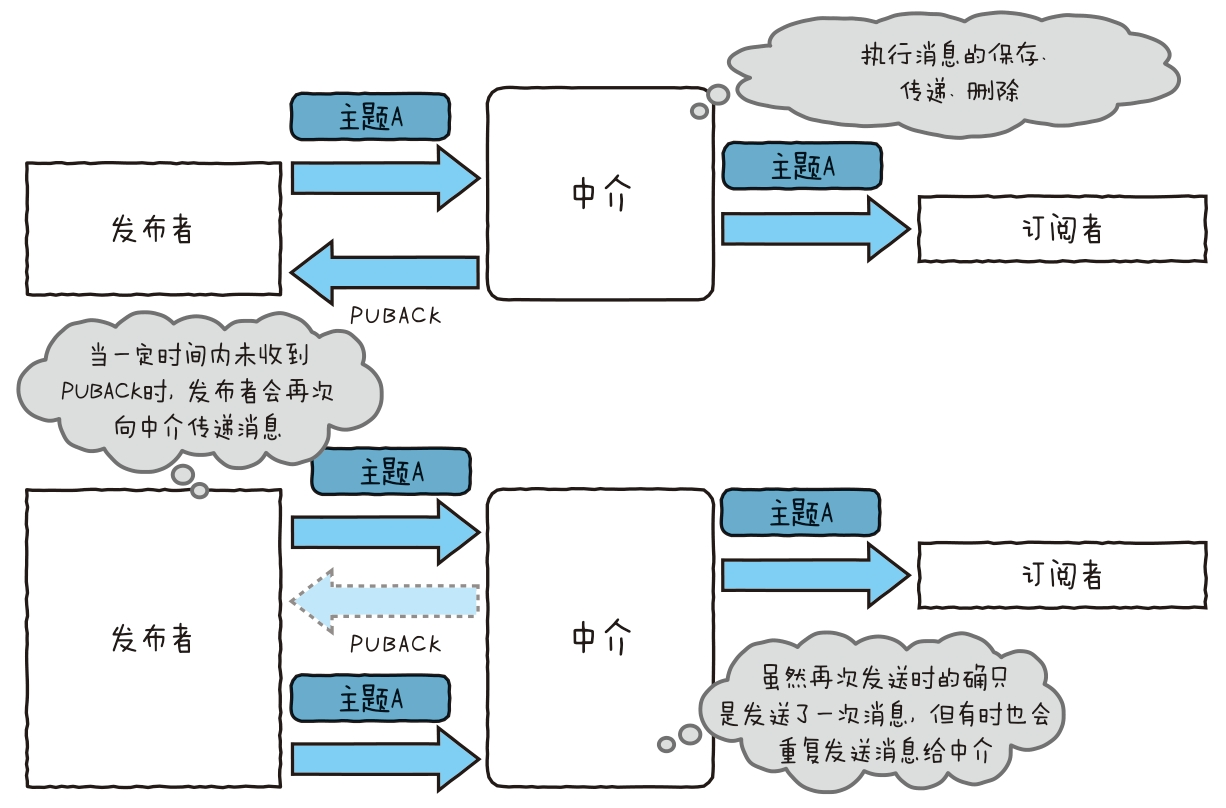
\includegraphics[width=1\linewidth]{31}
	\caption{QoS 1( 至少发送一次消息 )}
	\label{fig:1}
\end{figure}

最后是 QoS 2,它指的是准确发送一次消息(exactly once)。把它跟 QoS 1 合在一起使用,就能避免接收到重复的消息(图 2.13)。用QoS 2 发送的消息里面含有消息 ID。中介收到消息后会将消息保存,然后给发布者发送 PUBREC 消息。发布者再给中介发送 PUBREL 消息,然后中介会给发布者发送 PUBCOMP 消息。接下来中介才会依据订阅者指定的 QoS,向订阅者传递接收到的消息。

\begin{figure}[htbp]
	\centering
	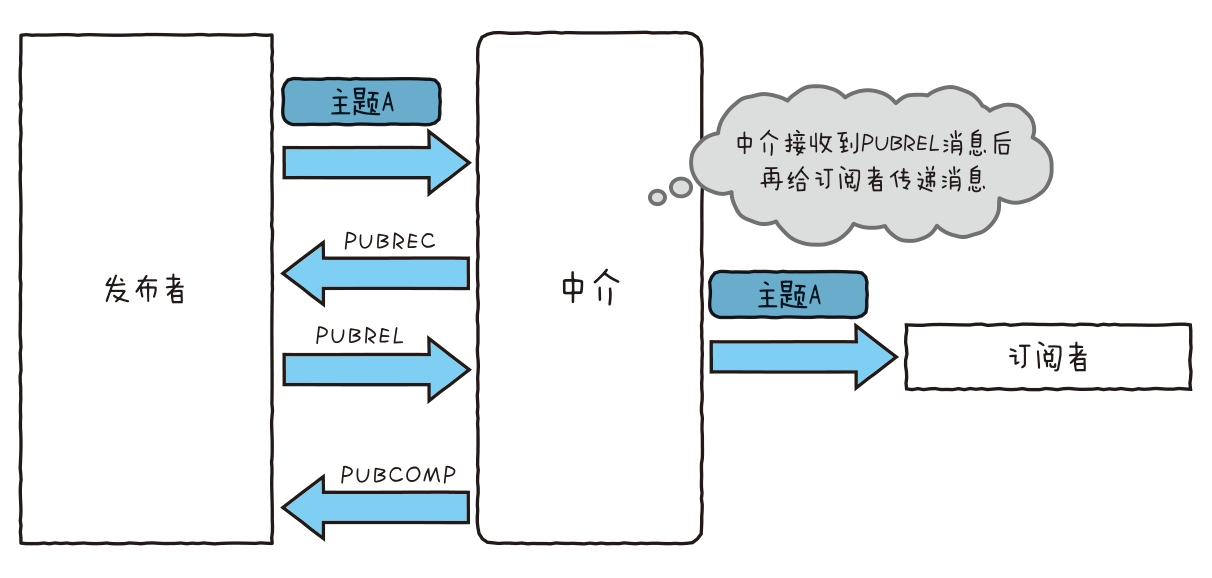
\includegraphics[width=1\linewidth]{32}
	\caption{QoS 2( 只发送一次消息 )}
	\label{fig:1}
\end{figure}

此外,就 QoS 2 而言,有时使用的中介会影响消息的传递时间。

人们通常使用的是 QoS 0,只有要确保信息发送成功时才使用 QoS 1 和 QoS 2,这样一来可以减少网络的负担。后文将会讲到 Clean session,其中 QoS 的设定也是非常重要的。

\subsubsection{Retain}

订阅者只能接收在订阅之后发布的消息,但如果发布者事先发布了带有 Retain 标志的消息,那么订阅者就能在订阅后马上收到消息。

当发布者发布了带有 Retain 标志的消息时,中介会把消息传递给订阅了主题的订阅者,同时保存带有 Retain 标志的最新的消息。此时,若别的订阅者订阅了主题,就能马上收到带有 Retain 标志的新消息
(图 2.14)。

\begin{figure}[htbp]
	\centering
	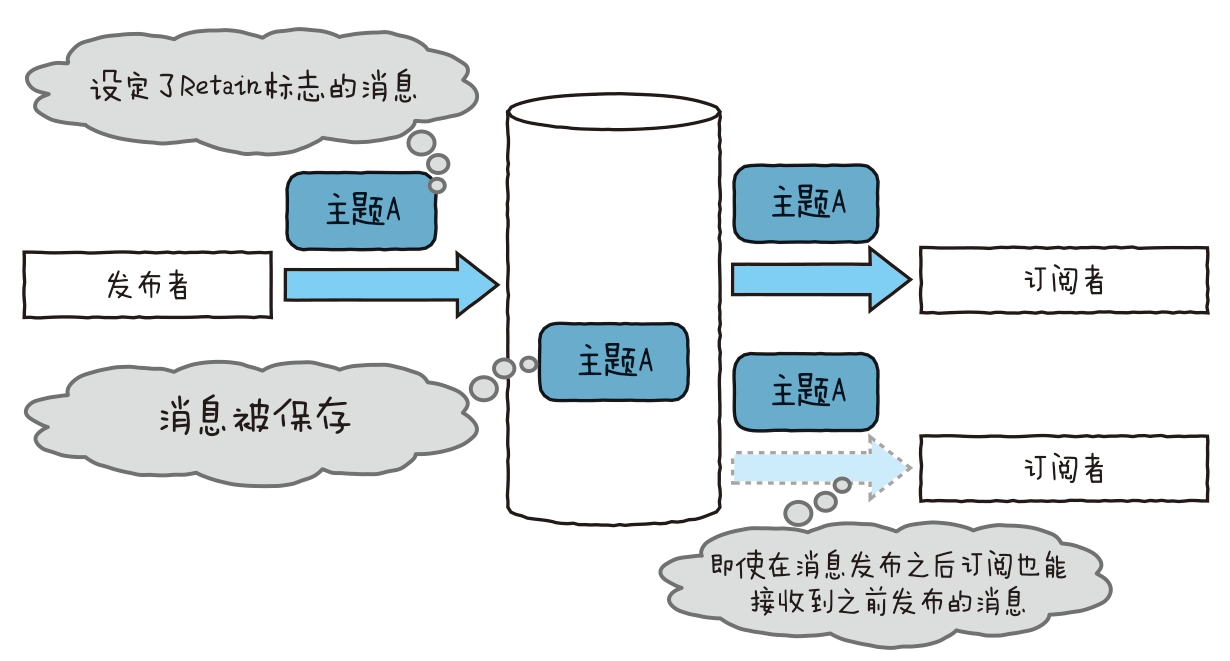
\includegraphics[width=1\linewidth]{33}
	\caption{Retain}
	\label{fig:1}
\end{figure}

\subsubsection{Will}

Will 有“遗言”的意思。由于中介的 I/O 错误或网络故障等情况,发布者可能会突然从中介断开,Will 就是专门针对于这种情况的一个机
构,它用于定义中介向订阅者发送的消息(图 2.15)。

\begin{figure}[htbp]
	\centering
	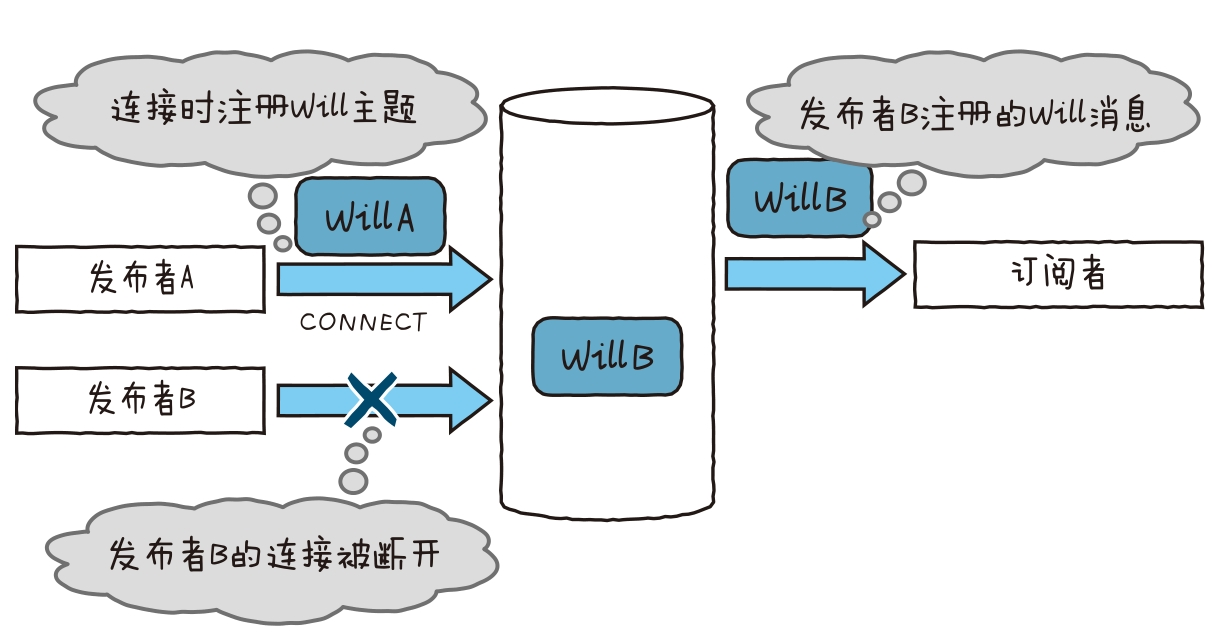
\includegraphics[width=1\linewidth]{34}
	\caption{Will}
	\label{fig:1}
\end{figure}

发布者在连接中介时会用到 CONNECT(连接)消息,连接时对其指定 Will 标志、要发送的消息以及 QoS。这样一来,如果连接意外断开,Will 消息就会被传递给订阅者。另外,还有一个标志叫作 Will
Retain。通过指定这个标志,就能跟前面说的 Retain 达到同样的效果,即在中介处保存消息。

当发布者使用 DISCONNECT(断开连接)消息明确表明连接已断开时,Will 消息就不会被发送给订阅者。

\subsubsection{Clean session}

Clean session 用于指定中介是否保留了订阅者的已订阅状态。用CONNECT 消息连接时,订阅者把 Clean session 标志设定为 0 或 1。0是保留 session,1 是不保留 session。

若指定 Clean session 为 0 且中介已经连接上了订阅者,则中介需要在订阅者断开连接后保留订阅的消息。另外,如果订阅者的连接已经断开,且发布者已经发布了 QoS 1、QoS 2 的消息给已订阅的主题时,中介则会把消息保存,等订阅者再次连接时发送给订阅者(图 2.16)。

\begin{figure}[htbp]
	\centering
	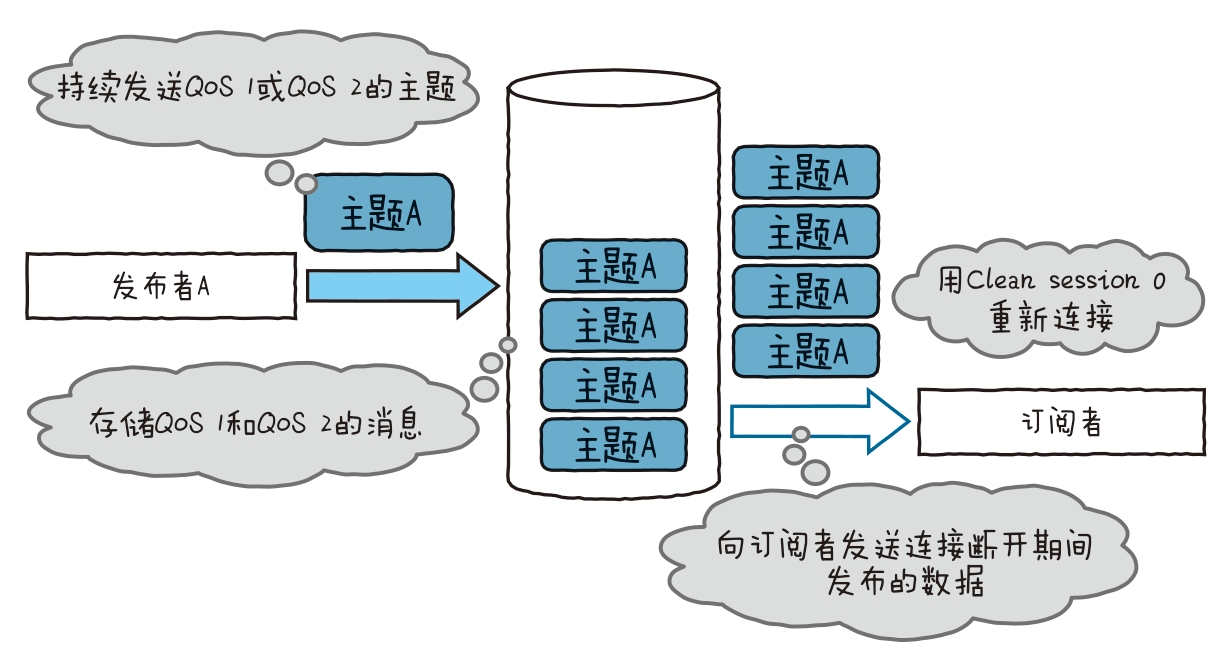
\includegraphics[width=1\linewidth]{35}
	\caption{Clean session}
	\label{fig:1}
\end{figure}

若指定 Clean session 为 1 并连接,中介就会废弃以往保留的客户端信息,将其当成一次“干净”的连接来看待。此外,订阅者断开连接时,中介也会废弃所有的信息。

我们可以用表 2.1 所示的几种产品来实现 MQTT。是否支持前文介绍的功能则取决于中介的种类。

\begin{table}[!ht] 
\centering
\caption{MQTT 的实现}
\begin{tabular}{|l|l|l|l|l|l|}
	\hline
	实现 & QoS & Retain & Will & Clean session & 其他 \\
	\hline
	ActiveMQ 5.10.0(支持插件) & 0、1、2 & 支持 & 不支持 & 不支持 & 有独立的指定主题的方法  \\
	\hline
	Apolo 1.7 &	0、1、2 &	支持 & 支持 & 支持 & —— \\
	\hline
	mosquitto 1.3.5 & 0、1、2 & 支持 & 支持 &	支持 & —— \\
	\hline
	RabitoMQ 3.4.3(支持插件) & 只有0和1 & 不支持 & 支持 & 支持 & —— \\
	\hline
\end{tabular}
\end{table}

除此之外,一个叫作 Paho 的库还公开了发布者和订阅者等客户端功能。不仅 Java、JavaScript、Python 配备了 Paho,连 C 语言和 C++ 都配备了 Paho。因此,我们能够将其与设备结合起来并加以使用。

\subsection{数据格式}

前面我们围绕用于接收数据的通信过程,即协议进行了讲解。事实上,数据就是通过协议来进行交换的。当然,就如我们前文所说,这条规则在物联网的世界里也是不变的。数据要经过协议进行交换,而数据的格式也很重要。通过 Web 协议来使用的数据格式中,具有代表性的包括 XML 和 JSON(图 2.17)。

\begin{figure}[htbp]
	\centering
	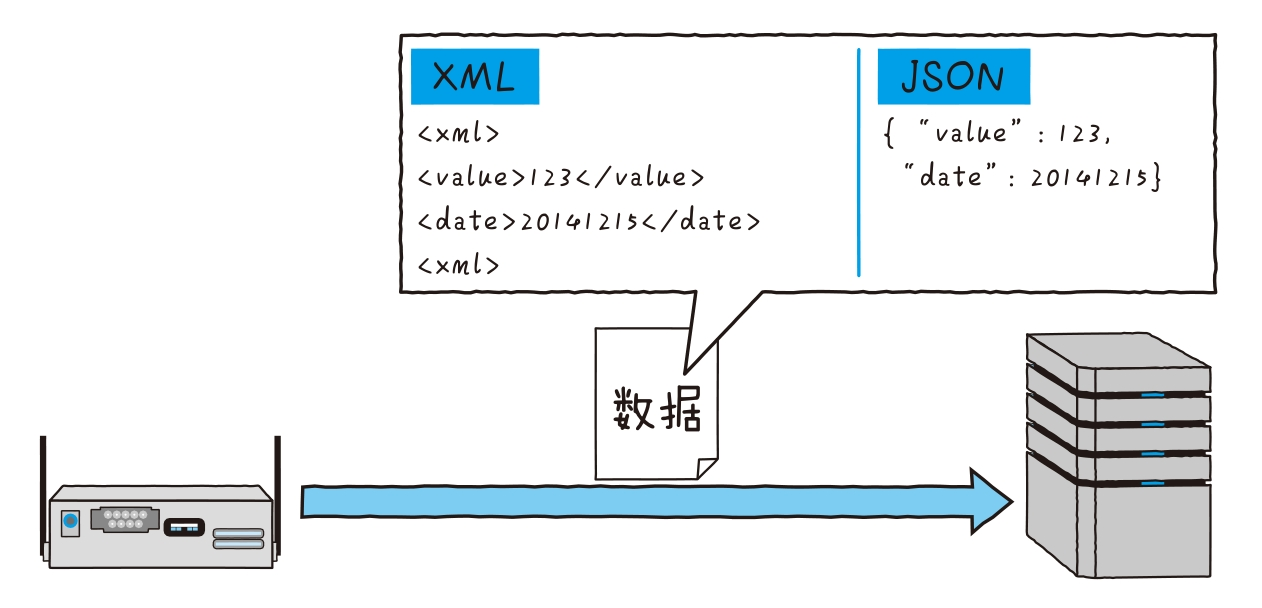
\includegraphics[width=1\linewidth]{36}
	\caption{具有代表性的格式}
	\label{fig:1}
\end{figure}

从物联网的角度来说,使用者也能很方便地使用 XML 和 JSON 。举个例子,假设设备要发送传感器的值,此时除了发送传感器的值以外,还要一并发送数据接收时间、设备的机器信息以及用户信息等数据。自然,设备还会通知多个传感器的值和机器的状态。这样一来,使用者就需要好好地把从设备发送来的数据结构化。

图 2.18 用 XML 和 JSON 分别表示了两台传感器的信息、设备的状态、获取数据的时间,以及发送数据的设备名称等。

\begin{figure}[htbp]
	\centering
	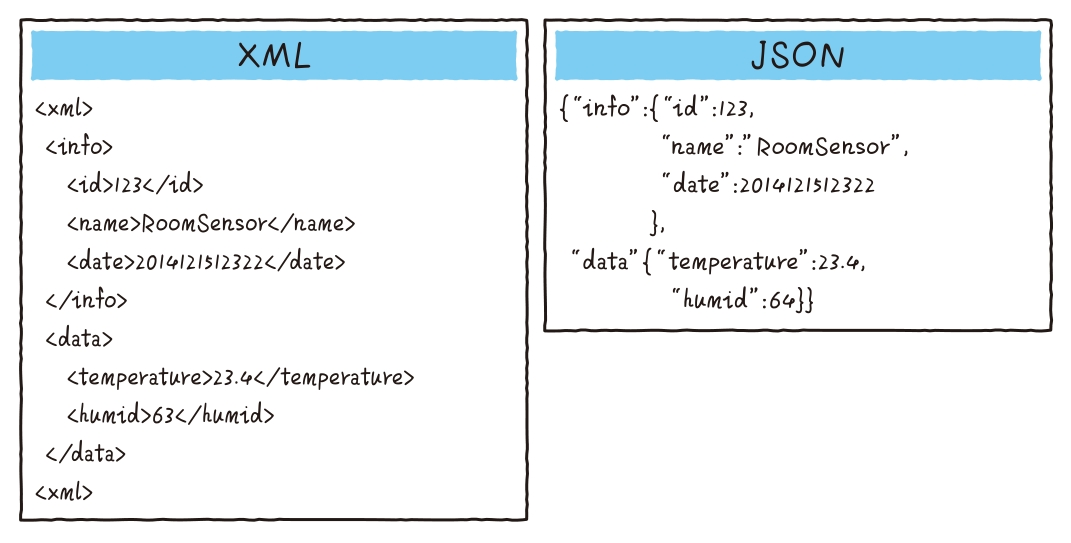
\includegraphics[width=1\linewidth]{37}
	\caption{传感器信息的示例(XML 和 JSON)}
	\label{fig:1}
\end{figure}

比较二者可知,XML 的格式比 JSON 更容易理解。然而 XML 的字符数较多,数据量较大。相对而言,JSON 比 XML 字符数少,数据量也小。

XML 和 JSON 这两种数据格式都在每种语言中实现了各自的库,使用者通过程序就能很轻松地使用这些库。那么到底使用哪种才好呢?关于这点我们不能一概而论,不过 JSON 数据量小,更适合使用移动线路等低速线路通信的情况。

设备传来的数据和 Web 不一样,大多是传感器、图像、语音等数值数据。相较于文本而言,这样的数据更适合用二进制来处理。不过,我们前文介绍的 XML 和 JSON 都是用文本格式来处理数据的。

基于物联网服务处理这些格式时,要把文本数据转换成数值数据和二进制数据。因此需要进行两项工作,即解析 XML 和 JSON 格式,以及把解析结果从文本格式转换到二进制形式。这样一来,就需要分两步来处理。

如果能直接以二进制形式接收数据,是不是就能更迅速地处理数据了呢?由此,一种数据格式应运而生,它就是 MessagePack(图 2.19)。

\begin{figure}[htbp]
	\centering
	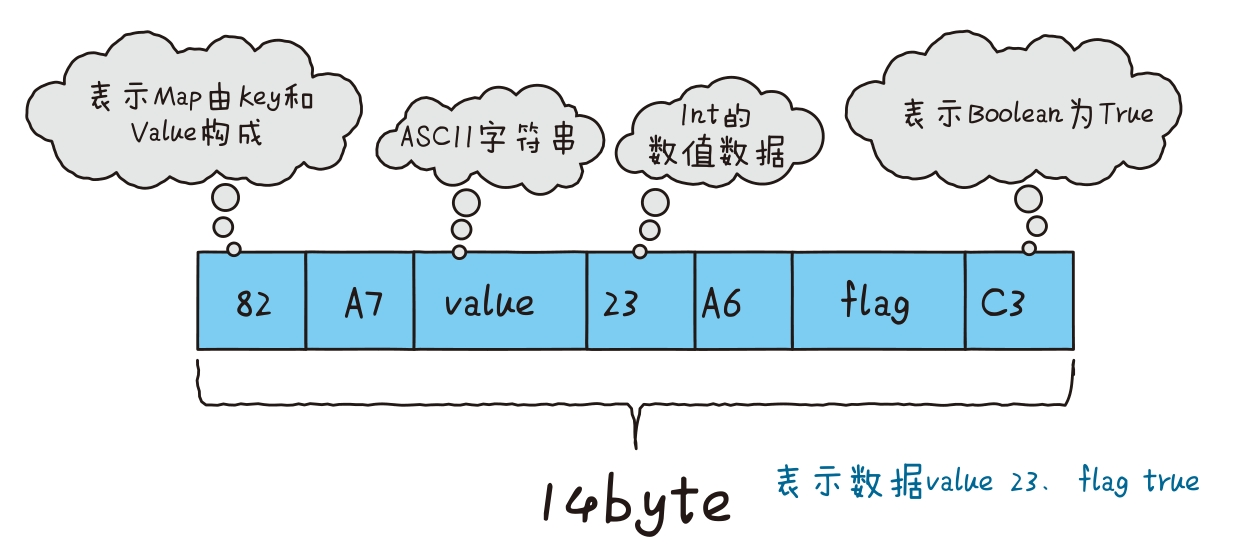
\includegraphics[width=1\linewidth]{38}
	\caption{使用 MessagePack 格式的传感器数据示例以及与 JSON 的对比}
	\label{fig:1}
\end{figure}

MessagePack 的数据格式虽然跟 JSON 相似,其数据却保留了二进制的形式。因此,虽然这种数据格式不方便人们直接阅读,但计算机却能很容易地处理。

又因为 MessagePack 发送的是二进制数据,所以比起以文本形式发送数据的 JSON,数据更加紧凑。MessagePack 跟 XML 和 JSON 一样,都提供了面向多种编程语言的库,另外,近年来多个 OSS(开源软件)也都采用了 MessagePack。

我们不能一口咬定哪种格式好,哪种格式不好,请各位根据要发送的数据的特性,来选择符合目的的数据格式。

\subsubsection{图像、语音、视频数据的处理}

传感器数据、文本数据”和“图像、语音、视频”的数据格式差别很大。拿图像、语音、视频来说,一条数据之巨大远远超过传感器数据,而且这些数据是二进制数据,很难转换成字符串,所以就很难用前面介绍的 XML 和 JSON 格式对它们进行处理。

用 HTTP 发送图像数据时,可以用 XML 或 JSON 格式记录拍摄时间和设备的信息,用 multi-part/form-data 格式来发送图像数据。然而,换成语音和视频时,就是一种时间上连续的数据。因此,我们在发送语音和视频数据时需要下一番工夫。

例如,需要把语音和视频分割成一个个小文件来发送。在用 HTTP 协议进行这项操作时,每次发送一个小数据都会生成一个会话。这样一来就能通过有效应用 WebSocket 等协议来减轻给物联网服务造成的负担了。这种情况下,使用者或许需要使用 MessagePack,或是定义一个专门用于处理二进制的格式。再或者,还能以用物联网服务进行语音和数据分析为前提,只在设备处提取用于分析的特征并发送,而不是把所有数据一并进行发送。大家在试图实现包含语音和视频数据的服务时,不妨考虑一下本专栏的思路。

\section{处理数据}

\subsection{处理服务器的作用}

很显然,处理服务器就是处理接收到的数据的地方。“处理”是一个抽象的词语,例如保存数据,以及转换数据以使其看上去更易懂,还有从多台传感器的数据中发现新的数据,这些都是处理。使用者的目的不同,处理服务器的内容也各异。不过说到数据的处理方法,它可以归纳成以下 4 种:数据分析、数据加工、数据保存以及向设备发出指令(图 2.20)。

\begin{figure}[htbp]
	\centering
	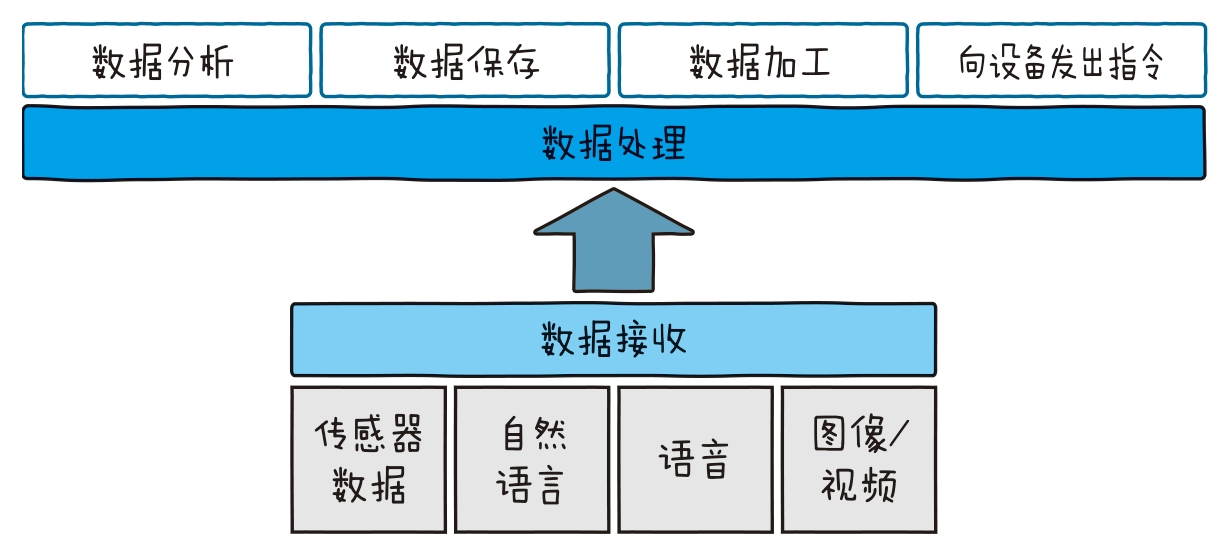
\includegraphics[width=1\linewidth]{39}
	\caption{数据的处理}
	\label{fig:1}
\end{figure}

关于数据的分析和加工,有两种典型的处理方式,分别叫作“批处理”和“流处理”。首先就来说说这个“批处理”和“流处理”。

\subsection{批处理}

批处理的方法是隔一段时间就分批处理一次积攒的数据。一般情况下是先把数据存入数据库里,隔一段时间就从数据库获取数据,执行处理。批处理的重点在于要在规定时间内处理所有数据。因此,数据的数量越多,执行处理的机器性能就得越好。

今后设备的数量将会增加,这一点在第一章已经解释过了。人们需要处理从数量庞大的设备发来的传感器数据和图像等大型数据,这被称为“大数据”。不过,通过使用一种叫作分布式处理平台的平台软件,就能高效地处理数兆、数千兆这种大型数据了。具有代表性的分布式处理平台包括 Hadoop 和 Spark。

\subsubsection{Apache Hadoop}

Apache Hadoop 是一个对大规模数据进行分布式处理的开源框架。Hadoop 有一种叫作 MapReduce 的机制,用来高效处理数据。MapReduce 是一种专门用于在分布式环境下高效处理数据的机制,它基本由 Map、Shuffle、Reduce 这 3 种处理构成(图 2.21)。

\begin{figure}[htbp]
	\centering
	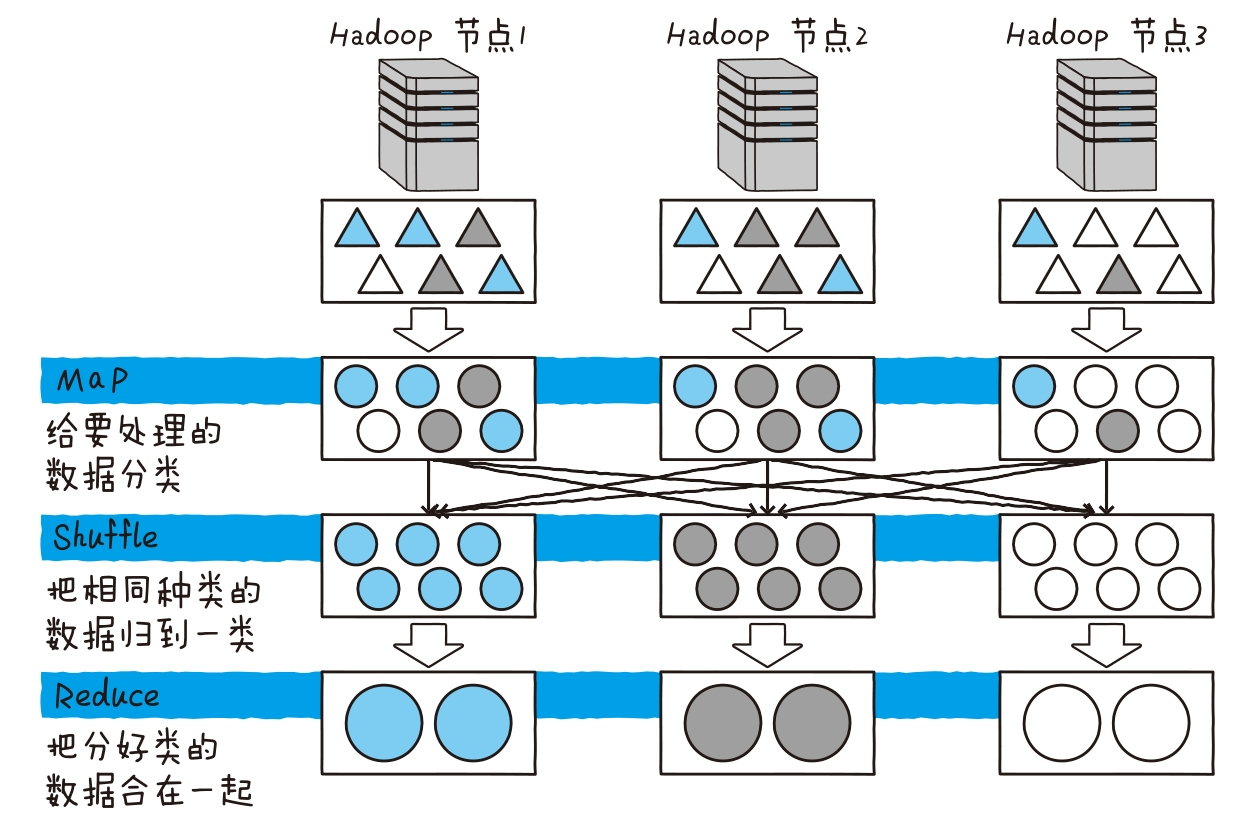
\includegraphics[width=1\linewidth]{40}
	\caption{通过 Hadoop MapReduce 执行批处理}
	\label{fig:1}
\end{figure}

Hadoop 对于每个被称为节点的服务器执行 MapReduce,并统计结果。首先是分割数据,这里的数据指的是各个服务器的处理对象。最初负责分割数据的是 Map。Map 对于每条数据反复执行同一项处理,通过 Map 而发生变更的数据会被移送到下一项处理,即 Shuffle。Shuffle 会跨 Hadoop 的节点来把同种类的数据进行分类。最后,Reduce 把分类好的数据汇总。

也就是说,MapReduce 是一种类似于收集硬币,按种类给硬币分类后再点数的方法。用 Hadoop 执行处理的时候,为了能用 MapReduce 实现处理内容,使用者需要下一番工夫。

另外,Hadoop 还有一种叫分布式文件系统(HDFS)的机制,用于在分布式环境下运行 Hadoop。HDFS 把数据分割并存入多个磁盘里,读取数据时,就从多个磁盘里同时读取分割好的数据。这样一来,跟从一台磁盘里读出巨大的文件相比,这种方法更能高速地进行读取。如上所述,如果使用 MapReduce 和 HDFS 这两种机制,Hadoop 就能高速处理巨型数据。

\subsubsection{Apache Spark}

Apache Spark 也和 Hadoop 一样,是一个分布式处理大规模数据的开源框架。Spark 用一种叫作 RDD(Resilient Distributed Dataset,弹性分布数据集)的数据结构来处理数据(图 2.22)。

\begin{figure}[htbp]
	\centering
	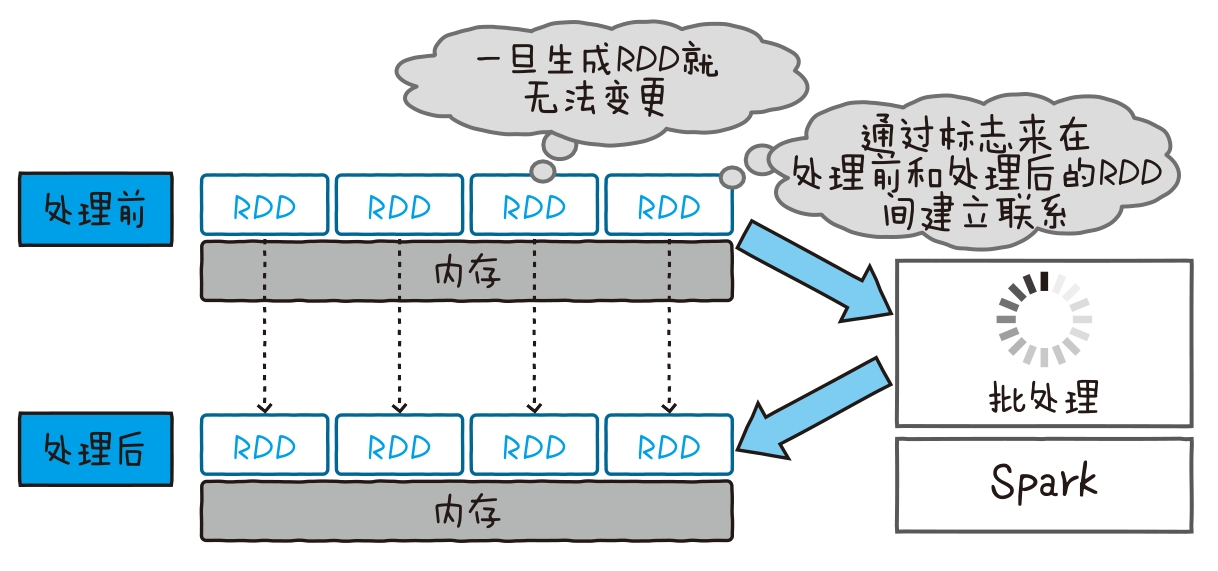
\includegraphics[width=1\linewidth]{41}
	\caption{通过 Spark 执行批处理}
	\label{fig:1}
\end{figure}

RDD 能够把数据放在内存上,不经过磁盘访问也能处理数据。而且 RDD 使用的内存不能被写入,所以要在新的内存上展开处理结果。

通过保持内存之间的关系,就能从必要的时间点开始计算,即使再次计算也不用从头算起。根据这些条件,Spark 在反复处理同一数据时(如机器学习等),就能非常高速地运行了。

对物联网而言,传输的数据都是一些像传感器数据、语音、图像这种比较大的数据。批处理能够存储这些数据,然后导出当天的设备使用情况,以及通过图像处理从拍摄的图像来调查环境的变化。随着设备的增加,想必今后这样的大型数据会越来越多。因此,重要的是学会在批处理中使用我们介绍的分布式处理平台。

\subsection{流处理}

批处理是把数据攒起来,一次性进行处理的方法。相对而言,流处理是不保存数据,按照到达处理服务器的顺序对数据依次进行处理。

想实时对数据做出反应时,流处理是一个很有效的处理方法。因为批处理是把数据积攒之后隔一段时间进行处理,所以从数据到达之后到处理完毕为止,会出现时间延迟。因此,流处理这种把到达的数据逐次进行处理的思路就变得很重要了。此外,流处理基本上是不会保存数据的。只要是被使用过的数据,如果没必要保存,就会直接丢弃。

举个例子,假设有个系统,这个系统会对道路上行驶的车辆的当前位置和车辆雨刷的运转情况进行搜集。

仅凭搜集那些雨刷正在运转的车辆的当前位置,就能够实时确定哪片地区正在下雨。此时,使用者可能想保存下过雨的地区的数据,这时候只要保存处理结果就好,所以原来的传感器数据可以丢掉不要,流处理正适用于这种情况。用流处理平台就能实现流处理。

流处理和批处理一样,也准备了框架。在这里就给大家介绍一下 Spark Streaming 和 Apache Storm 这两个框架。

\subsubsection{Spark Streaming}

Spark Streaming 是作为 Apache Spark(在“批处理”部分介绍过)的库被公开的。通过 Spark Streaming,就能够把 Apache Spark 拿到流处理中来使用(图 2.23)。

\begin{figure}[htbp]
	\centering
	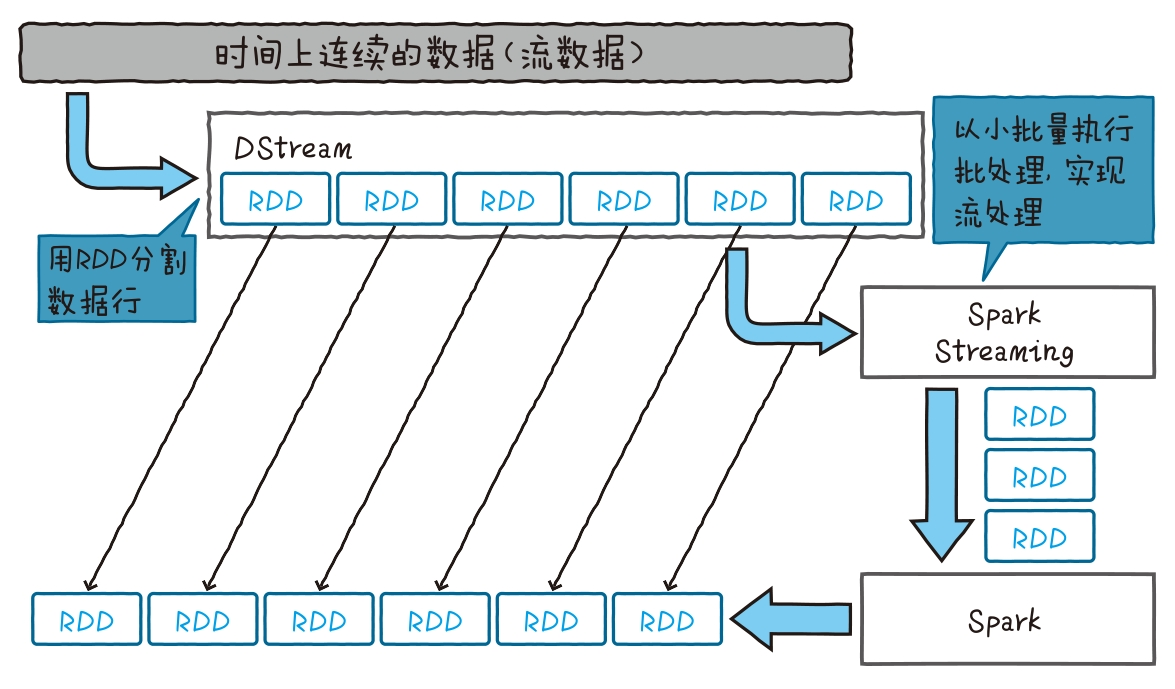
\includegraphics[width=1\linewidth]{42}
	\caption{通过 Spark Streaming 执行流处理}
	\label{fig:1}
\end{figure}

Spark Streaming 是用 RDD 分割数据行的,它通过对分割的数据执行小批量的批处理来实现流处理。输入的数据会被转换成一种叫作 DStream 的细且连续的 RDD。先对一个 RDD 执行 Spark 的批处理,将其转换成别的 RDD,然后按顺序对所有 RDD 反复执行上述处理来实现流处理。

\subsubsection{Apache Storm}

Apache Storm 是用于实现流处理的框架,结构如图 2.24 所示。

\begin{figure}[htbp]
	\centering
	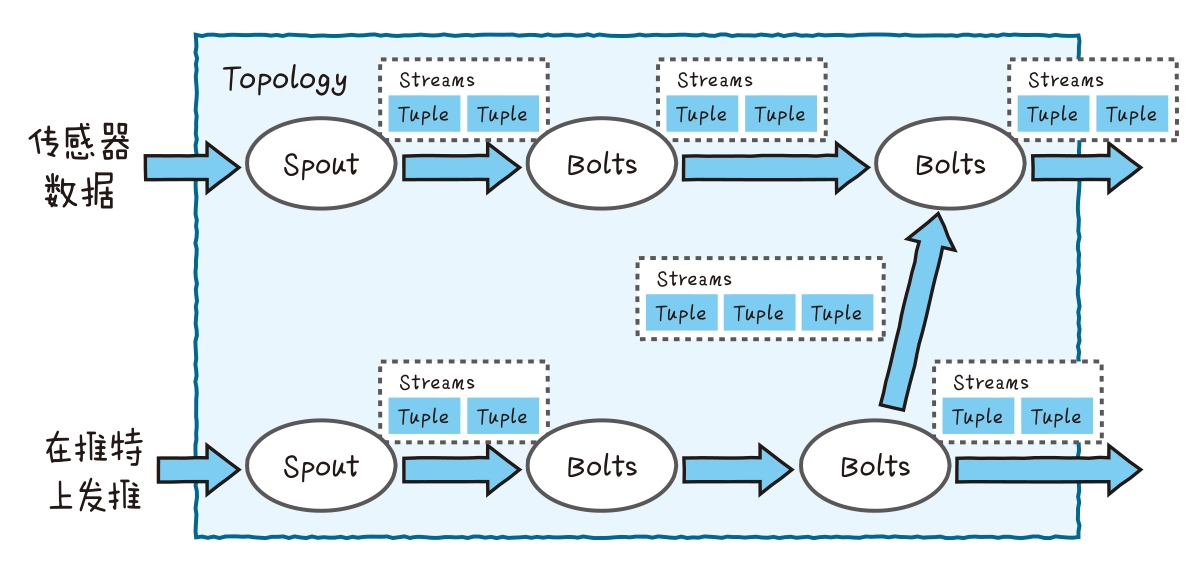
\includegraphics[width=1\linewidth]{43}
	\caption{Apache Storm 的结构}
	\label{fig:1}
\end{figure}

用 Storm 处理的数据叫作 Tuple,这个 Tuple 的流程叫作 Streams。

Storm 的处理过程由 Spout 和 Bolts 两项处理构成,这种结构叫作 Topology。Spout 从其他处理接收到数据的时候,Storm 处理就开始了。Spout 把接收到的数据分割成 Tuple,然后将其流入 Topology 来生成Streams,这就形成了流处理的入口。接下来,Bolts 接收 Spout 以及从其他 Bolts 输出的 Streams,并以 Tuple 为单位处理收到的 Streams,然
后将其作为新的 Streams 输出。可以自由组合 Bolts 之间的连接,也可以根据想执行的处理自由组合 Topology,还可以随意决定 Tuple 使用的数据类型,以及使用 JSON 等数据格式。

\section{存储数据}

\subsection{数据库的作用}

数据库的作用是保存并灵活运用数据(图 2.25)。除此之外,其作用还包括从保存的数据中找出与所指定条件相符的数据。另外,数据库还能把多条数据连在一起,把它们作为一个数据取出。

\begin{figure}[htbp]
	\centering
	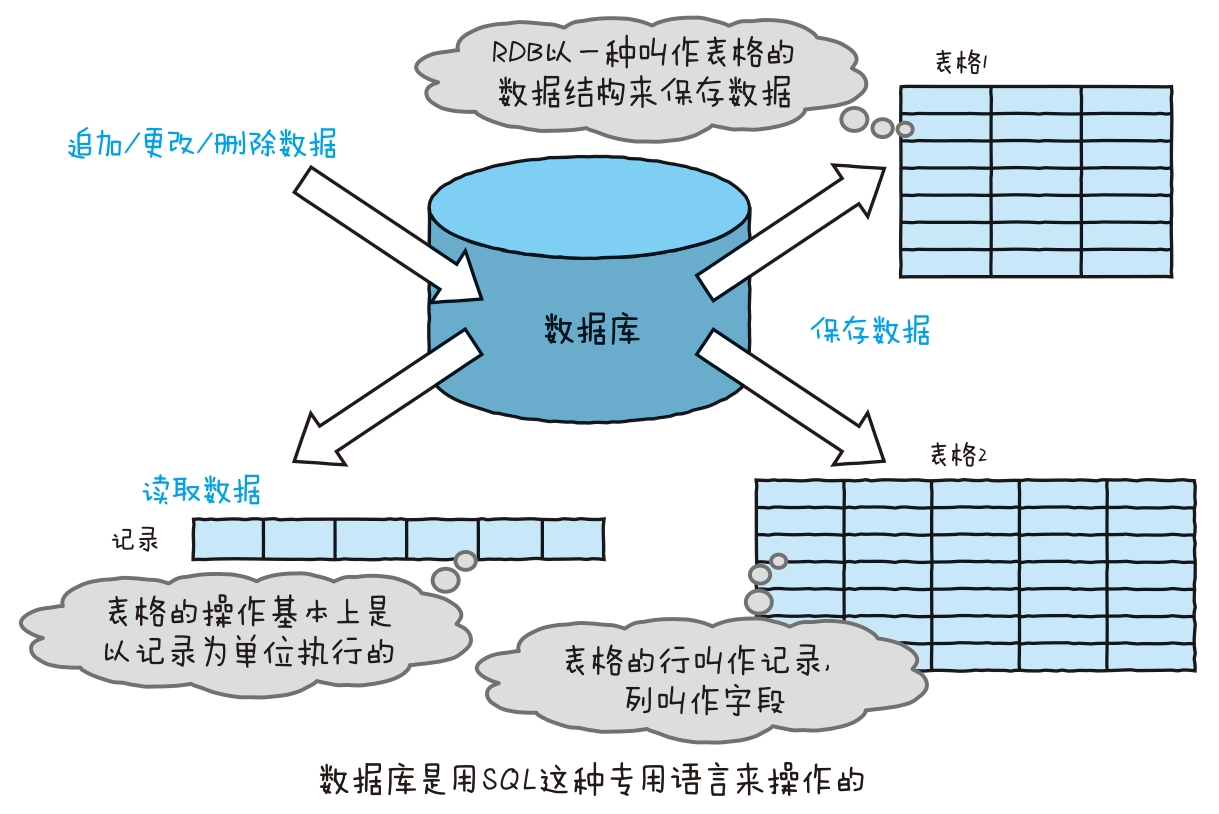
\includegraphics[width=1\linewidth]{44}
	\caption{数据库的作用}
	\label{fig:1}
\end{figure}

打个比方,已知与特定传感器相关的 ID,测量时间,以及温度传感器的值。光凭这些数据,是无法理解数据指的是哪个房间的温度的。因此就需要传感器的 ID 以及跟房间名字有关的数据。把这两条数据加在一起,才能知道某房间的温度。

图 2.25 展示的是一个叫作 RDB(关系数据库)的数据库。最近,除了 RDB 以外还出现了一种叫作 NoSQL 的数据库。

RDB 用一种叫作 SQL 的专门用来操作数据库的语言来保存和提取数据。另一方面,NoSQL 则是用 SQL 以外的各种方法来操作数据库。本书还会介绍键值存储(Key-Value Store,简称 KVS)和文档型数据库等种类的数据库。

\subsection{数据库的种类和特征}

这里我们一并为大家说明数据库的种类和特征,以及为了实现物联网服务而处理设备数据时的要点。

\subsubsection{关系数据库}

关系数据库是人们用得最普遍的数据库。如图 2.25 所示,关系数据库具备一种叫作表格的表格型数据结构,其用途在于存储数据库,使用者用 SQL 语言来对其执行数据的提取、插入以及删除。

SQL 是一种非常强大的语言,它能用非常简洁的表述写出命令,来把多个表格联系到一起,搜索符合目标条件的数据。此外,使用者还能通过多种多样的编程语言来使用 SQL。不过一旦确定了表格,就很难更改其结构了。因此,需要仔细考虑设备传来的数据性质再决定结构。

举个例子,假设由于传感器和设备的增加而导致一些必须保存的数据增多,此时,如果表格结构如图 2.26 所示,那么就很难再追加新的数据了。

\begin{figure}[htbp]
	\centering
	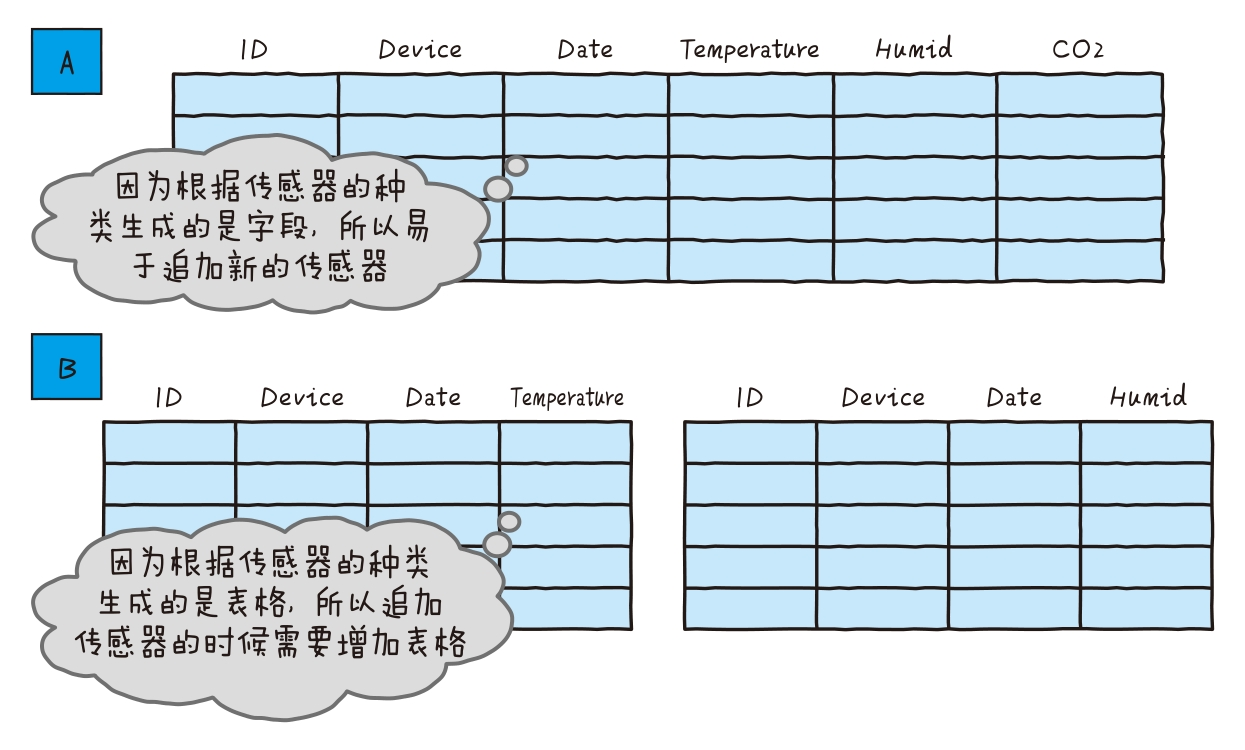
\includegraphics[width=1\linewidth]{45}
	\caption{以 RDB 的表格结构示例}
	\label{fig:1}
\end{figure}

在 A 表这种情况下,我们就必须变更表格的条目。而换成 B 表就没必要更改表格本身。不过,这样一来就需要生成一个新的表格。

因此,如图 2.27 所示,要生成一个结构来把所有传感器数据插入同一个字段里。采用这个结构时,即使来了新的传感器数据,也没有必要更改表格结构或是追加新的表格。不过传感器数据的类型必须是统一的,而且,这样一来就会在同一个表格里注册大量的数据。这种情况下,有时就得花一段时间才能从表格里检索到我们需要的数据。为了解决这个麻烦,数据库提供了一个叫作索引的机制。

\begin{figure}[htbp]
	\centering
	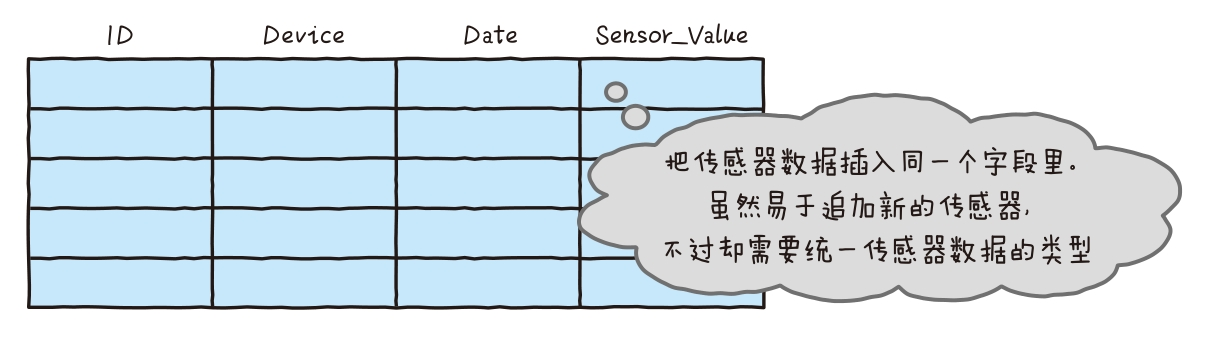
\includegraphics[width=1\linewidth]{46}
	\caption{用于保存传感器信息的表格结构示例}
	\label{fig:1}
\end{figure}

以上列举的表格就是一个例子。关于用哪种方法构成表格更好,我们不能一概而论,而是需要先考虑注册的是怎样的数据,以后又会积累多少数据,然后再下决定。

关系数据库也不擅长保存图像和语音等二进制形式的数据。虽然能够用一种叫作 BLOB(Binary Large Object,二进制大对象)的数据形式来达到保存的目的,不过,这也需要另费一番工夫,因为根据用途,有时需要把图像直接保存为文件,把图像的路径单独保存在 RDB 里(图 2.28)。

\begin{figure}[htbp]
	\centering
	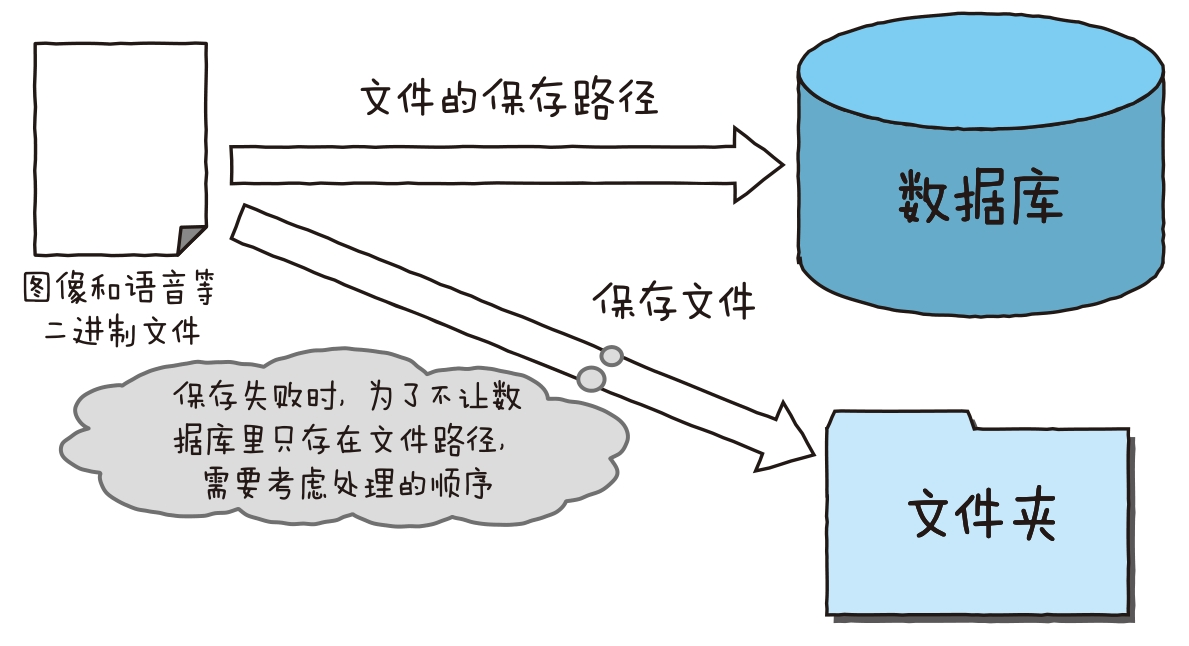
\includegraphics[width=1\linewidth]{47}
	\caption{用 RDB 处理图像和语音}
	\label{fig:1}
\end{figure}

数据库把数据保存到硬盘,因此经常会发生对硬盘的访问(磁盘 I/O)。这样一来,这步处理就比其他处理要慢。就系统中而言,这是处理速度方面容易产生瓶颈的一个地方。除了介绍的内容之外,还有一些需要大家注意的地方,希望大家加深对这部分内容的理解并将其灵活运用。

\subsubsection{键值存储}

键值存储属于 NoSQL 数据库的一种。NoSQL 是一种不使用 SQL 的数据库的统称。键值存储,就是把一种叫作“值”(value)的数据值,和能够一对一特定“值”的“键”(key)的集合保存在一起。

此外,还有把数据保存在内存里的键值存储,以及把数据保存在硬盘里的键值存储。前者一方面能够高速保存数据,而另一方面,因为数据是放在内存上的,所以软件停止运行的时候,原先保存的内容就会丢失。因此前者适合作为缓存来使用。而后者保存数据的速度虽然不及前者,但即使软件停止运行,数据也不会丢失。

有一种叫作 Redis 的键值存储,它具备前后两者的性质,在通常情况下它是把数据存储在内存上的,但在任何时间都能够把数据保存到硬盘。因此,它既能够高速执行存储,也能永久保存数据。

\subsubsection{文档型数据库}

文档型数据库和键值存储一样,都属于 NoSQL 数据库的一种。文档型数据库能以 XML 和 JSON 这种结构化文档的格式保存数据。特别是近年来,有一种叫作 MongoDB 的文档型数据库很受欢迎,它以JSON 的格式保存数据(图 2.29)。

\begin{figure}[htbp]
	\centering
	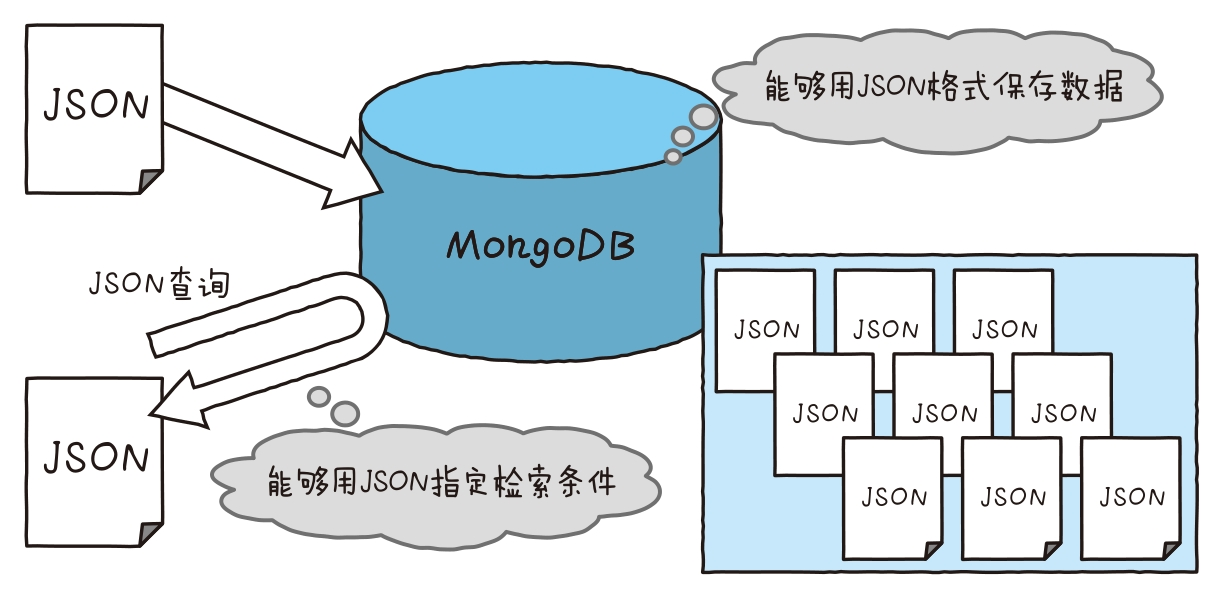
\includegraphics[width=1\linewidth]{48}
	\caption{文档型数据库 MongoDB}
	\label{fig:1}
\end{figure}

MongoDB 能够直接保存 JSON 格式的数据,还能用 JSON 的值进行检索。这样一来,在用 JSON 交换传感器的信息时,就能直接对数据进行保存和使用。即使增加了新的数据条目或是新增了设备,也能直接以JSON 格式保存数据,因此,不需要像 RDB 那样考虑表格的结构。非常
适合用于无法读出设备的数量和数据的种类等情况,以及保存传感器等设备的数据。

\section{控制设备}

\subsection{发送服务器的作用}

发送服务器的目的在于向设备发送数据并控制设备。发送服务器可以使用 2.3 节介绍过的 HTTP、WebSocket、MQTT 协议和数据格式。

发送服务器靠在 1.3.4 节提到过的两种方法来运行,一种是通过设备申请来发送数据的同步传输;另一种是由发送服务器在任意时间发送数据的异步传输。那么,就用 HTTP、WebSocket、MQTT 协议来看看如何实现同步和异步传输。

\subsection{使用 HTTP 发送数据}

要实现数据发送,HTTP 是最简单的方法。在这个方法里,发送服务器是等待接收 HTTP 请求的 Web 服务器。设备向这台服务器申请发送数据,作为响应,服务器把数据发给设备(图 2.30)。

\begin{figure}[htbp]
	\centering
	
\includegraphics[width=1\linewidth]{49}
	\caption{通过 HTTP 发送数据}
	\label{fig:1}
\end{figure}

使用者需要定期从设备执行轮询连接。采用此方法的原因主要有以下两个。

原因一:无法确定唯一地址,例如无法给设备设定全局 IP 地址等。这种情况下,发送服务器就不知道应该把数据发送给哪台设备了。

原因二:考虑到设备频繁断电和移动线路的传输费用。此时,设备没有持续连接网络。即使设备已经连接过网络,但只要没有持续连接,那么,即使发送服务器执行了发送数据的操作,也发不到设备那里去(图 2.31)。

\begin{figure}[htbp]
	\centering
	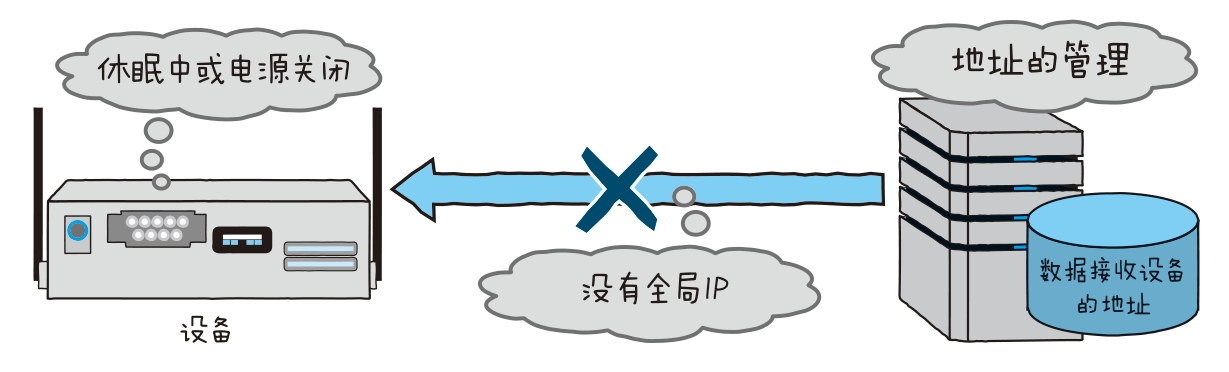
\includegraphics[width=1\linewidth]{50}
	\caption{服务器端发送数据困难}
	\label{fig:1}
\end{figure}

\subsection{使用 WebSocket 发送数据}

使用 WebSocket 时,需要用设备连接发送服务器,并确立 WebSocket 连接。只要建立了一次 WebSocket 连接,就能实现从发送服务器和客户端发送数据。

\subsection{使用 MQTT 发送数据}

前文介绍了 HTTP 和 WebSocket,它们采用的方法都是由设备访问发送服务器。就这些方法而言,只要客户端没有发出申请,数据就不会被发送。当然使用者也可以在设备上建立 HTTP 和 WebSocket 协议,由服务器来连接设备。不过,一旦增加了设备,服务器想管理所有设备就相当困难了。

针对这点,我们来试着看一下这种服务器:它灵活运用 MQTT,并且发挥了发布 / 订阅模型的优点。使用 MQTT 时的发送服务器如图 2.32 所示。

\begin{figure}[htbp]
	\centering
	\includegraphics[width=1\linewidth]{51}
	\caption{通过 MQTT 发送数据}
	\label{fig:1}
\end{figure}

首先设备作为订阅者,向 MQTT 中介进行订阅。然后,发送服务器则是发布者,同样向中介进行发布。这样一来,发送服务器只需要把确定的数据加在主题上发送就行了,发送服务器和设备都不需要知道彼此的地址。只要知道中介的地址,就能够实现通信。一旦订阅者断开,中介就会负责在断开时发送通知,并在重新连接时再次发送数据。

通过灵活运用 MQTT 的功能,构建发送服务器就变得简单多了。

\subsubsection{事例:面向植物工厂的环境控制系统}

这里为大家介绍一个事例。近年来盛行向农业领域导入 ICT 技术。特别是在生产过程中,在高龄化背景下,为了确保新的农业劳动力和提高生产力,ICT 技术的广泛运用备受期待。以往,环境控制都是由农户手工测量塑料大棚内的温湿度,以及控制植
物的生长状况,现在则把重点放在实现完全自动化,以提高生产力上。

采用各种传感器来测量和记录(相当于接收数据)温度、湿度、二氧化碳及光照等数据。这样就能把环境条件数值化,再记录一下在已测量的环境条件下作物实际的生长质量。通过这样循环,就能提取某个作物的生长模式(相当于数据分析)。这样一来,只要明确了应该调整哪些环境条件,就能在培育过程中,把从环境中感测到的数据和设定的阈值进行比较(相当于数据处理),从而实现自动控制空调,自动注入二氧化碳(相当于发送数据)。

人们正在试图通过搭建这样的架构,以实现 ICT 技术的大规模化,使法人加入农业模式变得更加简单。如果继续推进这样的措施,那么,或许在未来的某一天,当农业劳动者想培育这种品质的蔬菜时,只要按下一个按钮就能实现自动栽培,接下来等几
个月后收获就可以了。

\chapter{物联网设备}

\section{设备——通向现实世界的接口}

\subsection{为什么要学习设备的相关知识}

经过前两章的学习,想必各位读者已经掌握物联网这个词描绘出的世界和用于实现物联网的系统架构了。基于这点,这一章将会为大家介绍在物联网世界中起着核心作用的因素,即设备的相关知识。

可能有人会觉得自己没有必要学习设备的机制,但是,请这样认为并想赶快读完本章的读者稍稍放慢速度,因为本章正是为了那些以往没有从事过设备开发的读者们编写的。

而且,所有的工程师都有必要加深对设备的理解,因为这关系到“连通性”给设备开发带来的变化。这里我们就先来看看这些变化。

\subsection{连通性带来的变化}

很显然,智能手机和随身听等伴随大家日常生活的设备都是由硬件和软件组成的。硬件经过了精致的设计,软件则用来控制硬件。设备开发的本质就是在最大限度上实现硬件和软件的完美配合。

对于平日里从事 Web 应用程序开发的各位软件工程师来说,提到设备开发,或许大家就会有一种敬而远之的感觉。在考虑独立开发某种设备的时候,肯定会有人担心以下这些问题。

● 是否需要对硬件有深入的了解

● 开发设备控制软件是否需要专业知识

● 开发硬件是否需要特殊的开发环境

就结论而言,这些问题的答案很统一:需要。就像大多数人都知道的那样,用于控制设备的软件有一个明确的种类,那就是“嵌入式软件”。开发嵌入式软件需要极强的专业性,即使是在物联网的世界,这一本质也基本没有什么变化。

那么,物联网会带来哪些改变呢?解开这个问题的关键词就是“连通性”。连通性一词表示的是机器和系统间的相互连接性和结合性。物联网设备试图经由网络来“连接”外部系统,并通过以下技术革新让以往人们无法想象的一些设备都具备了连通性(图 3.1)。

● 硬件的进化使设备的小型化和高级化得以发展

● 能够在广域条件下轻易地利用高速度 / 高品质网络的环境得以实现

\begin{figure}[htbp]
	\centering
	\includegraphics[width=1\linewidth]{52}
	\caption{连通性给设备带来的变化}
	\label{fig:1}
\end{figure}

有些设备不具备连通性,这很正常,因为它们本身就是用来独立实现功能的。而且,这种设备一旦出了库就没法再变更商品规格了,所以需要花大把的时间和成本来开发。

一方面,物联网设备本身的结构非常简单,提供的是一种与云服务或智能手机等外部机器组合在一起的一体化服务。这种情况下,用于设备的应用程序能够很轻松地得到更新,在产品发布后还能一边从用户处获取反馈,一边不断改良软件(包括设备自身的固件)。此外,还能够在云端对大量的设备信息进行整合和加工,以一个应用程序为接口向用户提供有益的信息。

另一方面,硬件开发本身的成本竞争正在不断激化,设备开发必然会促进设备自身的高级化。而围绕设备开发,将服务整体作为一个生态系统来进行最适宜的设计规划,其重要性则不言而喻。想必在这股潮流中,存在差异性的部分也将会多元化。例如,构建算法,来为用户提供统一处理从设备处采集到的信息并进行高级分析的服务;或者构建应用程序,来实时反映设备不断变化的情况等。这些物联网设备的与众不同之处也必定会显现出来。

为了尽最大努力回应这种需求并无缝开发应用了物联网设备的服务,从事开发(设备本身的开发,连接设备的云端系统以及利用它们提供服务的应用程序等的开发)的工程师在开发的同时要达成共识,这点是非常重要的。在这个过程中,在软件开发高速化的牵引下,用以往难以想象的硬件开发速度不断开发和提供服务才是需求所在。要想实现这个目标,服务开发者和设备开发者都必须正确理解彼此在各自领域都是如何工作的(图 3.2)。

\begin{figure}[htbp]
	\centering
	\includegraphics[width=1\linewidth]{53}
	\caption{在开发物联网设备过程中相互理解的重要性}
	\label{fig:1}
\end{figure}

本章将会依据采用了物联网设备的服务开发所固有的特性,紧扣各位读者在新开发物联网设备及使用了物联网设备的服务时会遇到的各种各样的关键点,并针对设备的结构提取重点内容来进行解说。此外,本章还会介绍如何用“原型设计”在轻松搭建设备的同时评价以及审查产品与服务。

\section{物联网设备的结构}

\subsection{基本结构}

物联网设备的种类五花八门,但其结构一般都如图 3.3 所示。物联网设备跟普通的机械产品一样,都包含用于检测用户操作和设备周边环境变化的输入设备,提示某些信息或者直接作用于环境的输出设备,以及作为设备的大脑来负责控制机器的微控制器等。另外,物联网服务还有一个不可或缺的条件,那就是连接网络。接下来将为大家简单介绍这些要素。

\begin{figure}[htbp]
	\centering
	\includegraphics[width=1\linewidth]{54}
	\caption{物联网设备的基本结构}
	\label{fig:1}
\end{figure}

\subsubsection{微控制器}

微控制器是微型控制器(Micro Controller)的略称,是一块控制机器的 IC(Integrated Circuit,集成电路)芯片。它能够编写程序,并根据描述的处理读取端子状态,或者向连接上的电路输出特定信号。

微控制器由内存(用于存储程序和保存临时数据)、CPU(用于执行运算处理和控制)以及外围电路(包含与外部的接口,以及计时器等必要的功能)构成。(图 3.4)

\begin{figure}[htbp]
	\centering
	\includegraphics[width=1\linewidth]{55}
	\caption{微控制器的结构}
	\label{fig:1}
\end{figure}

在实际使用微控制器时,需要串行端口和 USB 等各种接口以及电路等。如果想自己制作设备,那么通过使用微控制器,以及安装了以上要素、名为“微控制器主板”的电路板,就能很轻松地开发硬件了。虽说每种产品的规格各有不同,但基本上是以图 3.5 所示的流程进行开发的。

\begin{figure}[htbp]
	\centering
	\includegraphics[width=1\linewidth]{56}
	\caption{微控制器的开发流程}
	\label{fig:1}
\end{figure}

现在大部分电子产品都搭载有微控制器。打个比方,请想象一个冰箱(图 3.6)。冰箱内部能够达到某个目标温度,是因为微控制器里写有一个程序,这个程序的作用就是监视连接在微控制器输入端子上的温度传感器的状态,并控制制冷机以达到目标温度。利用传感器测量和判别信息就叫作感测。

\begin{figure}[htbp]
	\centering
	\includegraphics[width=1\linewidth]{57}
	\caption{微控制器的应用示例(冰箱)}
	\label{fig:1}
\end{figure}

物联网的流行跟微控制器主板的变化也有关系。过去,为了把微控制器主板连接到网络,需要每个开发者独立实现接口,而近年来微控制器主板的种类逐渐增多,包括以外部连接模块来提供连接网络功能的微控制器主板,以及标配型微控制器主板。这样一来,开发出的设备就能轻松连接到网络。这种开发环境的完善正在不断进行。如果利用这种微控制器主板,即使没有开发过硬件的人,也能够向设备开发发起挑战。

下一节将详细介绍微控制器主板的类型和用法。

\subsubsection{输入设备}

为了让设备获取周边情况和用户操作等信息,必须在机器上实现传感器和按钮等元件(电子器件)。

举个例子,假设有台智能手机,那么这台手机都搭载了什么样的传感器呢?各位读者应该注意到了,实际上它搭载了触摸屏、按钮、相机、加速度传感器、照度传感器等相当多的感测设备(图 3.7)。这些传感设备能帮助我们更详细且精细地掌握周边的情况。反言之,又因为传感器的类型和精度极限在一定程度上决定着机器的性能,所以在设备开发过程中,传感器的选择是非常重要的一步。

\begin{figure}[htbp]
	\centering
	\includegraphics[width=1\linewidth]{58}
	\caption{各种输入设备}
	\label{fig:1}
\end{figure}

\subsubsection{输出设备}

物联网想要实现的不只是感测状态,将状态“可视化”。对人类和环境进行干涉,控制世界令其向目标状态发展才是其真实目的。

在需要向用户反馈某些信息时,显示器、喇叭、LED 这些用于输出信息的设备就会发挥作用(图 3.8)。就像前文说的那样,物联网设备重在小型和简便。如何配置这些输出设备能让其高效地把信息传达给用户,无疑是设计阶段非常重要的课题。

\begin{figure}[htbp]
	\centering
	\includegraphics[width=1\linewidth]{59}
	\caption{各种输出设备}
	\label{fig:1}
\end{figure}

还有一个方法是在设备上安装驱动器,让驱动器物理性地作用于环境。驱动器是通过输入信号来实现控制的驱动装置的统称。例如具有代表性的伺服电机,它能够根据输入的电子信号把电机转动到任意的角度。这个方法和机器人技术有着密切的联系,与网络联动“运行”的设备属于当今最受瞩目的领域之一(第 8 章会讲到机器人)。

3.5 节将会为大家讲解如何控制与微控制器相连接的输出设备。

\subsubsection{与网络相连接}

关于连通性在物联网设备中的重要性,已经为大家说明过了。物联网设备通过网络与服务器进行通信,积累和分析感测到的信息,通过远程操作控制设备。因此,设备就需要有用于连接网络的接口。

网关机器和设备之间存在无线连接和有线连接两种连接形式,这两种连接形式又存在多种连接方法。

如果制造的设备是需要固定的机器,比如用来监视室内环境的传感器或是相机等,就可以采用有线连接。虽然需要考虑线路的排布问题,不过这种方法通信较为稳定。

如果制造的设备是便携式设备,比如可穿戴设备等,就需要考虑采用无线连接了。比起有线连接,采用无线连接时,设备的应用范围更广,不过使用前还需要考虑到障碍物所导致的通信故障,以及电源的装配等因素。

使用者应该根据不同设备的特性来选择连接形式。关于连接形式的详细内容,我们将会在 3.3 节详细介绍。

\subsection{微控制器主板的类型和选择方法}

\subsubsection{选择微控制器主板的出发点}

在设备开发中,微控制器主板的选择是一个非常重要的因素。根据开发环境、想制造的设备以及经验的不同,设备“适合”的微控制器主板是不一样的。

就像前文说的那样,微控制器在写入程序之后才可使用,所以硬件本身还能再次利用。如果您是出于原型设计的目的“想做个试试看”而购买了微控制器,那么,为了之后还能将其沿用于其他项目,推荐您先购买具备通用结构的微控制器。

表 3.1 列举的几个关键点可以作为具体的选择标准来参考。

\begin{table}[!ht] 
	\centering
	\caption{微控制器的选择标准}
	\begin{tabular}{|l|l|}
		\hline
		选择标准 & 详细内容 \\
		\hline
		产品规格 & 检查接口、内存、耗电量等。在多个设备开发项目中使用时,I/O端口(输入输出端子)越多越易于扩展。 \\
		\hline
		成本 & 虽然初学者没有必要购入高价的设备,不过对新手而言,如果购入了某种程度上比较通用的设备,那么大多数情况下,就能节省后期补买器件的工夫,这样一来最终花费的成本就很低 \\
		\hline
		尺寸 & 微控制器主板的尺寸很大程度上会影响设备的大小。使用尺寸较小的微控制器主板时,I/O 端口的数量也会受限,所以最好要考虑规格和尺寸的平衡 \\
		\hline
		开发环境 & 易于连接 PC 的设备,或是配备有开发软件的设备在一开始都比较容易上手。是否能使用已经掌握的开发语言也是一个重要的标准 \\
		\hline
		信息的可获得性 & 如果是初学者,建议选择能从 Web 网站和图书等上面获取信息的设备。日本产品都公布了日语文档,使用者不擅长英语也能放心使用。此外,从采集信息方面来看,交流的活跃度也是一个重要的出发点 \\
		\hline
	\end{tabular}
\end{table}

与设备的变化相呼应,微控制器主板的样式也在不断地推陈出新(图 3.9)。

过去,微控制器主板的目标在于搭载单片机,实现结构的简约性和高通用性。与此相对,能用在移动电话和智能手机上的高性能 CPU、完善的 I/O 端口,以及配备了网络接口的超微型计算机,即单板计算机等设备陆续登场。使用者不但能通过 Linux 操作系统来运行这些单板计算机,还能像控制以往的微控制器那样控制 I/O 引脚(pin)。微控制器主板和计算机的分界线正在逐渐模糊。

\begin{figure}[htbp]
	\centering
	\includegraphics[width=1\linewidth]{60}
	\caption{以往的微控制器主板和单板计算机}
	\label{fig:1}
\end{figure}

单板计算机给未曾开发过硬件的软件开发者们提供了一个友好的开发环境。这些产品确实在一定程度上降低了开发初期技术上、心理上以及金钱上的难度。

当然,在实现商品化的过程中,为了能够适应大批量生产,需要削减无用的规格,实现价格的低廉化。在这一阶段以及未来,都需要用单片机来实现结构的最小化。也就是说,嵌入式开发自身的难度和需要的知识是没有变化的。不过单板计算机实现了原型设计过程的高速化和不断重复。尤其对于追求创新概念的物联网设备开发来说,重要的是不断地去重复试错。

本节将基于前文介绍的选择标准,来介绍几个具有代表性的微控制器。

\subsubsection{H8 型微控制器主板}

H8 型微控制器主板是一种单片机主板,它上面安装了瑞萨科技公司制造的 H8 型微控制器系列产品。在秋叶原和邮购电子器件的网站都可以轻易买到这种组装品。它是日本生产的,文档和手册内容充实,对于需要使用微控制器来制作电器的人来说,H8 型微控制器主板是一件标配品,在日本国内长期受到人们的喜爱,且售价 3000 日元,价格适中,初学者也能轻松购入。

与 PC 连接时,一般采用串行通信。近来,很多 PC 上都不设置串行端口了,不过这种情况下,可以采用 USB 串行转换线来连接 PC。在组装品中,有些配件需要使用者自己来安装,比如用于串行通信的端口等。根据数据表,把微控制器主板的接头和 D-SUB 9 针的插口接上就行,并没有什么难度。

虽然大多数情况下,开发是由附带的软件来进行的,不过采用的开发语言一般都是 C 语言。嵌入式开发更是大多都采用 C 语言。这是因为比起一般的计算机,单片机在规格方面(如内存和时钟数等)受到种种制约,从高效运用硬件资源的角度来说,多数情况下需要编写位操作和寻址等接近硬件操作的功能。

把 H8 作为学习嵌入式软件基础的入口是一个非常不错的选择,这样一来就能构建所有类型的硬件了。不过,如果“初学者想在短期内做出能运行的设备”,那么说实话还有些困难,建议大家结合自己的技术背景和学习目的来做选择。

\subsubsection{Arduino}

\begin{figure}[htbp]
	\centering
	\includegraphics[width=1\linewidth]{61}
	\caption{Arduino 主板}
	\label{fig:1}
\end{figure}

Arduino 是一款可以让没有从事过电子仪器设计和制作的人也能马上着手开发的微控制器主板,有着非常高的人气。它被应用在美术和个人爱好等各种领域,作为一个容易上手的全方位平台受到了人们的喜爱。

但是 Arduino 这个词指的不单单是微控制器主板,它还是对 Arduino 主板,以及最适合于 Arduino 主板的综合开发环境—— Arduino IDE 的统称。Arduino 以“开放硬件”的理念为本,从硬件到软件所有的设计信息都是公开的,衍生出来的各种各样的产品也在市面上销售。

Arduino 非常便宜,只要 3000 日元,去秋叶原的电子器件店或是通过网购都能轻松购买到 Arduino。

Arduino 主板品种和规格繁多,其中最为标准的主板就是 Arduino UNO(图 3.10)。数字输入输出端子、模拟输入端子、USB 端口等单纯的 I/O 端口都被压缩在了一块小小的电路板上,买到手后马上就能开始开发设备。

另外,这块电路板还能扩展,使用者通过安装一个叫作 Shield 的对应器件就能追加功能。只要使用 Wi-Fi Shield、以太网 Shield、GSM Shield 等,就能轻松搭建出一个用于连接网络的环境。除此之外,市面上还有传感器和具备多种功能的 Shield 产品,请各位务必查一查。

Arduino 最大的特征就在于它开发的简易性。只要用 USB 线连接 Arduino 主板和 PC,开发环境就搭建完成了。编写程序和写入主板则通过 Arduino IDE(图 3.11)来完成。开发是用类似于 C++ 的 Arduino 语言来进行的。开发前,Arduino IDE 已经准备了很多的示例代码,有软件开发经验的使用者只要看一看就能大概明白该怎么使用。即使是新手,也有可能在开箱后 10 分钟以内做好一个能让 LED 闪烁的电路和程序。

虽然 Arduino 有这么多让人啧啧称赞的规格,但它有一个大问题,那就是跟 Shield 一起搭配使用的话尺寸也会增大。Arduino 的大小会决定设备的大小。因为将 Arduino 用于教育也属于制造 Arduino 的一个目的,所以人们很重视其通用性。虽然其结构固然比采用 H8 微控制器等时要大,但从商品化观点来说,当前要单独使用 Arduino 还有些困难。

\begin{figure}[htbp]
	\centering
	\includegraphics[width=1\linewidth]{62}
	\caption{Arduino IDE}
	\label{fig:1}
\end{figure}

这里,原型工具有多棒就不必多说了。拿能以最低开发成本构建硬件这点来说,原型工具就是最适合用于试做的产品。对硬件开发有兴趣的人不妨尝试着接触一下。

\subsubsection{Raspberry Pi}

Raspberry Pi 是一款搭载有 ARM 处理器的单板计算机,由英国 Raspberry Pi Foundation(树莓派基金会)开发(图 3.12)。Raspberry Pi 的出现无疑给烧得正旺的单板计算机热潮再添了一把火,它也因此而著名,但其实 Raspberry Pi 原本是为编程教学而开发的。

其系列产品包括 Raspberry Pi 1 model A、A+、B、B+ 以及 Raspberry Pi 2 model B 这 5 种。这 5 种产品搭载的端口和内存等规格都不同,在此,就以最新型号 Raspberry Pi 2 model B 为例给大家介绍一下。

不管如何,开发者设计 Raspberry Pi 的主要目的都是想把它当作计算机来使用,因此,除了 USB 端口、声音影像输入输出端口、以太网端口等输入输出端口外,使用者还能通过 microSD 卡等外部存储器来连接 Raspberry Pi。从搭载了 GPU 这点也能看出来,开发者的初衷是把它连接到显示器当作 PC 来使用。另外 Raspberry Pi 还安装有 Debian 类
Raspbian 操作系统,标准支持 Python。从 Raspberry Pi 2 model B 开始,Raspberry Pi 的 CPU 就是四核处理器了,并宣布支持 Windows 10。作为一个能实现多种应用程序的平台,Raspberry Pi 备受瞩目。

\begin{figure}[htbp]
	\centering
	\includegraphics[width=1\linewidth]{63}
	\caption{Raspberry Pi 2 model B}
	\label{fig:1}
\end{figure}

如果想把 Raspberry Pi 当成微控制器主板来用,那么没有模拟输入端子可以说是其一大缺点。虽然和传感器等设备直接连接时需要输入模拟信号(详细情况会在后面说明),但 Raspberry Pi 只能接受数字输入方式。为了处理模拟信号,需要通过 A/D 转换电路把模拟信号转换成数字信号,并连接到输入端口。虽说市面上也有专用的电路板,不过这样就会增加多余的成本。

价格来说,Raspberry Pi 2 model B 售价 4200 日元,比 Arduino 稍微贵一些,但比之后要说明的 Beagle Bone Black 便宜。作为单板计算机来说,Raspberry Pi 2 model B 是一款物美价廉的产品,不过如果想拿它当微控制器,还需要做不少准备下不少工夫。话虽如此,关于这款产品,能参考的信息还是非常多的(如图书等),还请各位一定要尝试一下。

\subsubsection{Beagle Bone Black}

\begin{figure}[htbp]
	\centering
	\includegraphics[width=1\linewidth]{64}
	\caption{Beagle Bone Black}
	\label{fig:1}
\end{figure}

Beagle Bone Black(BBB)是德州仪器公司主持开发的一款搭载了 ARM 处理器的单板计算机(图 3.13)。这块主板的惊人之处在于平衡了微控制器主板和 PC 的性能。

作为硬件,Beagle Bone Black 除了搭载有 2×46 的 I/O 引脚,还具备 512 MB 的内存,4 GB 的集成闪存,以及以太网、microHDMI、USB、microSD 等丰富的输入输出端口。跟 Arduino 相比,Beagle Bone Black 的运算处理能力占据压倒性优势地位,能安装种类更多且自由度更高的软件。

此外,就软件而言,Beagle Bone Black 还能从 SD 卡安装任何 Linux 操作系统的发行版本,能够轻易而灵活地为开发者搭建出一个他们需要的软件开发环境。

就开发环境而言,用 USB 把 BBB 连接到 PC 来安装驱动后,就能从 PC 的浏览器访问名为 Cloud9 IDE 的 IDE。用这个 IDE 就能够通过 Node.js 来简单地进行行为描述。此外,因为它还能通过命令行来操作各个输入输出引脚的状态,所以能够将其作为脚本来进行行为描述。

BBB 有非常丰富的规格,跟我们介绍的其他主板相比,这款主板尺寸稍微大一些,作为商品化产品来使用不免有些困难,这一点跟Arduino 一样。其价格在 7000 日元左右,定价比一般的微控制器主板要高一些。

此外,中文资料不够丰富也是一个难点,对初学者来说可能会比较费劲。从国际角度来看,Beagle Bone Black 这款产品受到了比较活跃的开发者团队的支持,所以只要有决心去“啃”官方网站和 Wiki 这类网站来填补其不足,Beagle Bone Black 还是一款非常具有魅力的产品的。

\subsubsection{英特尔 Edison}

\begin{figure}[htbp]
	\centering
	\includegraphics[width=1\linewidth]{65}
	\caption{英特尔 Edison}
	\label{fig:1}
\end{figure}

在物联网开发中具备独树一帜的存在感的就是英特尔 Edison(图 3.14),它搭载了具备双核双线程的英特尔 Atom CPU,以及 100 MHz 的微控制器英特尔 Quark。这个主板的亮点在于彻底地改善了专为物联网设备设置的规格。

跟 Raspberry Pi 和 BBB 一样,英特尔 Edison 也标准安装了 Linux 操作系统(Yocto Linux)。除了具备作为 PC 最基本的功能以外,它还标准安装了 Wi-Fi 和蓝牙 4.0。在物联网设备中有两点是必备的,即节省空间的设计和连通性的实现。英特尔 Edison 极其袖珍,只有35.5 mm×25.0 mm×3.9 mm,但却具备了接通电源就能用 SSH 远程登录的功能,对比以往的微控制器主板,英特尔 Edison 的性能可谓惊人(图 3.15)。

\begin{figure}[htbp]
	\centering
	\includegraphics[width=1\linewidth]{66}
	\caption{英特尔 Edison 跟笔的比较}
	\label{fig:1}
\end{figure}

英特尔 Edison 主机带有 GPIO 引脚,但因为太小,所以不容易直接开发。英特尔为开发者准备了 Breakout Board Kit 和英特尔 Edison Kit for Arduino(Arduino 兼容板)两种扩展板,将主机插入扩展板之后就可以进行开发(图 3.16)。除了 I/O 引脚,扩展板上还安装有 SD 卡和 micro USB 端口,microSD 端口等,能够轻易地与外部设备相连接。此外,Arduino 兼容板和 Arduino UNO 两者引脚的配置基本相同,可以直接装配使用面向 Arduino 开发的主板和 Shield。

\begin{figure}[htbp]
	\centering
	\includegraphics[width=1\linewidth]{67}
	\caption{英特尔 Edison Kit for Arduino(Arduino 兼容板)}
	\label{fig:1}
\end{figure}

在软件开发环境方面,英特尔 Edison 也准备了多样且方便的环境(图 3.17)。

初学者一开始使用 Arduino IDE 入门会比较容易,它是专门为 Edison 量身定做的。通过 USB 线把 Edison 连接到 PC,就能通过 IDE 描述代码,往主板中写入信息,进行调试。对于用 Arduino 从事过开发的人来说,开发环境以及所有实现了 Arduino 兼容的环境,都是非常容易上手的。

又因为 C 语言和 C++ 的交叉编译程序已经公开了,所以只要用于开发的 PC 与 Edison 在同一个 Wi-Fi 网络里,就能通过 SSH 把在开发专用的 PC 上编译好的执行文件发送给 Edison 使用。

除此之外,英特尔 Edison 还标准安装了 Python 和 Node.js,开发者能够从众多选项中选择符合自己需要的来使用。特别是英特尔 XDK IoT Edison,如果想实现一个能用 Node.js 来控制硬件的环境,用它是再适合不过了。

\begin{figure}[htbp]
	\centering
	\includegraphics[width=1\linewidth]{68}
	\caption{英特尔 Edison 的开发环境}
	\label{fig:1}
\end{figure}

在灵活运用 Edison 方面有一点很重要,那就是 Edison 的用途不限于原型设计(图 3.18)。虽然在开发初期是使用扩展板来进行原型设计的,不过当产品规格在一定程度上确定了,也有望会量产时,通过制作产品的连接板也可以直接在产品上安装 Edison 主机。从避免发生大规模的规格变更(如在从原型设计到商品化的期间变更处理器)的角度而言,这点非常重要。

\begin{figure}[htbp]
	\centering
	\includegraphics[width=1\linewidth]{69}
	\caption{从原型设计到商品化的无缝过渡}
	\label{fig:1}
\end{figure}

虽然 Edison 有这么多富有魅力的规格,但比起其他主板,它的价格要略高一些。Edison 本身单卖就要 7000 日元,如果再和 Arduino 兼容板配套,就得花上 12 000 日元。而且每个引脚的输出电压都非常低,只有 1.8 V,很难跟其他设备直接连接运行。所以还得在连接电路上花一番心思才行。

因为这次介绍的都是比较新的产品,所以信息较少也在所难免,不过大家可以通过那些活跃的开发者团队来获取信息。因为还牵扯到Arduino兼容的问题,所以很多地方都应该能挪用 Ardunio 的知识技巧。如果能正确理解其优点与缺点,那么对物联网设备开发而言,Edison 会是一个非常优秀的开发平台。

\subsubsection{微控制器主板间的比较}

目前为止,各位已经看过几个不同类型的产品了。如今,微控制器和单板计算机的分界线日益模糊,为了迎合人们的需要,开发环境也变得多样化。只要比较一下前面介绍的微控制器主板就会发现,它们各自的目标领域还是有着微妙的差别的(图3.19)。

\begin{figure}[htbp]
	\centering
	\includegraphics[width=1\linewidth]{70}
	\caption{每个产品在概念上的差异}
	\label{fig:1}
\end{figure}

像 Arduino、英特尔 Edison 以及 BBB 这些都是适用于原型设计,而且在通用性和扩展性的平衡方面表现优秀的产品。而 Raspberry Pi 的目标是被当作 PC 使用,所以没有能直接指向设备的模拟 I/O 引脚。

另外,像 H8 系列这样的传统型微控制器,虽然在追求结构最小化这点上出类拔萃,但是一旦涉及连接网络等方面,可以说就比较鸡肋。

这样看来,英特尔 Edison 作为面向物联网设备开发的微控制器主板,不仅标准安装了 Wi-Fi 和蓝牙,还全面涵盖了原型设计和商品化,其存在感越来越强烈了(图 3.20)。

\begin{figure}[htbp]
	\centering
	\includegraphics[width=1\linewidth]{71}
	\caption{微控制器主板间的比较}
	\label{fig:1}
\end{figure}

\subsubsection{开源硬件的兴起}

相对于开源软件而言,Arduino、Beagle Bone Black、Raspberry Pi 等被称为开源硬件。开源硬件和 3D 打印等生产技术革新一同受到了人们的瞩目,因为它们像一串钥匙,开启的那扇大门通向一个能够自由而容易地开发产品的世界。近来以美国西海岸为首,新型硬件公司正在全世界逐步兴起,以前文我们介绍的种种产品为主,方便用户的(准确地说是方便开发者的)开发工具正不断出现,它们的出现给硬件开发的工艺创新带来了不可忽视的影响。

\section{连接“云”与现实世界}

\subsection{与全球网络相连接}

有两种让设备连接到网络的方式,一种是由设备本身直接连接全球网络,另一种是在本地区域内使用网关来连接全球网络(图 3.21)。近来,“生活记录”型的设备越来越多,其结构更接近前面说的第二种方式,例如通过蓝牙把可穿戴设备和智能手机配对,通过智能手机向服务器发送数据。

\begin{figure}[htbp]
	\centering
	\includegraphics[width=1\linewidth]{72}
	\caption{网络连接形式}
	\label{fig:1}
\end{figure}

与物联网设备相比,网关设备的硬件结构大多比较丰富,有的还支持再次发送数据和保存部分数据等功能。另外,网关设备还支持高级加密及数据压缩,在需要保证数据传输的安全性时,采用网关无疑是一个明智之选。

另一方面,直接连接网络时,则需要在物联网设备端实现再次发送等错误处理程序。虽然这点还需斟酌,不过如果采用直接连接方式,构建系统时就不用在意是否存在网关了。这样一来就能单纯地建立设备和服务器之间的连接了。

\subsection{与网关设备的通信方式}

物联网设备和网关设备进行通信的方式有很多种,既有有线的也有无线的。因为每种方式都各有利弊,所以需要大家根据设备的用途和特性来进行选择。

选择的标准包括通信时能够使用的协议、通信模块的大小、耗电量,等等。

在这里我们看一下各连接方式的特征。

\subsection{有线连接}

\subsubsection{以太网}

以太网连接方式采用网关设备和以太网电缆进行有线连接。这种方式不仅不怕无线电频率干扰,能够稳定通信,而且还有一大亮点,那就是能实现普通的 IP 通信协议,跟 PC 进行简单通信。

说到缺点,则包括终端要在一定程度上具备丰富的执行环境(如单板计算机),以及尺寸容易偏大,设置场所受限等。

\subsubsection{串行通信}

串行通信连接方式是指采用 RS-232C 等串行通信来连接其他设备。这个方式的优点包括多数工业产品配备了用于串行通信的端口,容易与现有产品建立连接等。使用 RS-232C 串口时,设备大多使用 D-SUB 9 针端口(图 3.22)。如果网关设备也有串行端口,那么就能用 RS-232C 串口线直接连接设备来进行通信。这里的线包括直通线和交叉线两种,请大家按照设备的结构进行选择。

相反,如果网关设备上没有串行端口,就得用“USB转串口线”来连接了。请各位注意,在这种情况下网关设备里必须安装有与转换芯片
(转换芯片在转换线里)对应的驱动程序。如果安装了与 FTDI 芯片(转换芯片的事实标准)对应的驱动软件,就比较容易找到对应的线了(关于驱动程序,会在下一节讲解)。

想实现串行通信,就需要在收发信息的两方设定表示通信速度的参数“比特率”,以及要发送数据的大小。

C 语言、Java、Python 这些常用的编程语言都准备了这种串行通信程序库,是一个很好用的接口。

\begin{figure}[htbp]
	\centering
	\includegraphics[width=1\linewidth]{73}
	\caption{D-SUB 9 针端口}
	\label{fig:1}
\end{figure}

\subsubsection{USB}

USB 是一个为大家熟知的接口。USB 的插头形形色色,但是在连接网关的时候,多数情况下跟计算机一样,采用一种叫 Type-A 的插头。此外,USB 有多种规格,每种规格传输数据的速度都不相同(表 3.2)。

\begin{table}[!ht] 
	\centering
	\caption{USB 的规格、传输速度及供电能力}
	\begin{tabular}{|l|l|l|}
		\hline
		名称 & 最大数据传输速度 & 供电能力 \\
		\hline
		USB 1.0 & 12Mbit/s & —— \\
		\hline
		USB 1.1 & 12Mbit/s & —— \\
		\hline
		USB 2.0 & 480Mbit/s & 500mA \\
		\hline
		USB 3.0 & 5Gbit/s & 900mA \\
		\hline
		USB 3.1 & 10Gbit/s & 100mA \\
		\hline
	\end{tabular}
\end{table}

要使用通过 USB 连接的设备,就得安装一种叫作设备驱动的软件。因此,用 USB 控制设备和接收数据时,有没有提供与设备对应的驱动就很重要了。打个比方,假设我们想把 USB 相机连接到网关来发送图像。如果想发送给 PC,单纯安装 USB 相机和相机的驱动就行了,而换成网关就不一样了。如果网关是在 Linux 上运行,那么就需要准备Linux 专用的驱动,制作获取图像的软件。

USB 在 PC 等通用机器上非常普及,其特征在于,比起 D-SUB 9 针等端口,这种端口的小尺寸占据了压倒性优势。

\subsection{无线连接}

\subsubsection{Wi-Fi}

如果采用 Wi-Fi 连接方式,通过 Wi-Fi 接入点就能够连接网络。通过它,可以在不便进行有线连接的环境中,实现移动型设备和 PC 及智能手机的联动,也就能更加容易地搭建出一个与本地区域内其他设备联动的系统了。

为了防止无线电频率干扰,需要注意接入点的设置。以下这些是所有无线连接方式都会面对的情况,那就是需要在安装设备的应用程序时考虑到通信断开的情况,例如先把数据保存在内部,等能连接上的时候再一口气发送过去等,这点工夫还是要费的。

此外,因为和蓝牙 4.0(后文再叙述)相比,Wi-Fi 耗电量高,所以不适合那些需要长时间进行通信的设备。

\subsubsection{3G/LTE}

3G/LTE 连接方式是通过移动运营商的通信线路来连接网络的。只要从运营商购买 SIM 卡,再把 SIM 卡插入设备里就能够通信了。

采用这种连接方式时,只要在信号范围内就能连接上网络,不需要像 Wi-Fi 那样去在意接入点的设置。相反地,在工厂和地下这类信号不好的地方就无法通信了。

想使用 3G/LTE,设备上需要配备用来插入 SIM 卡的插槽,这个条件大大地限制了硬件设计的发挥。除此之外,还会持续产生接入费用,所以也会对设备本身的价格与使用形式产生影响,例如采用月付费模式。另外,在某些情况下,开发终端是需要经过运营商审查的,这点请大家注意。

\subsubsection{蓝牙}

蓝牙是一种近距离无线通信标准,多数智能手机和笔记本电脑都有配备蓝牙。

2009 年,蓝牙 4.0 首次公开,它以内置电池的小型设备为主要应用对象,整合了超低功耗的 BLE(蓝牙低能耗,Bluetooth Low Energy)技术。根据设备的结构不同,它甚至可以实现靠一枚纽扣电池连续运行数
年。此外,原本的蓝牙和 Wi-Fi 一样采用 2.4 GHz 频段,容易产生干扰,但是从 4.0 起,这个问题已经得到了大幅度的改善。

除了一对一通信,BLE 还能实现一对多通信,通信机器只要在物联网设备附近且能使用 BLE,就能通过广播发送任意消息了。从 iOS7 起,iOS 就利用这种通信形式标准配备了 iBeacon 功能,iBeacon 能够测算环境中设置的 BLE 信号发送器,即 Beacon 的大概位置和 ID 信息(图3.23)。这项功能可以给店铺附近的顾客发送最适合他们的广告和优惠券。这种方法也作为一种新的 O2O(Online to Offline :一种服务和方法,通过这种服务和方法可以实现 Web 网站和应用程序等线上信息与线下店铺销售的联动)服务而备受瞩目。

\begin{figure}[htbp]
	\centering
	\includegraphics[width=1\linewidth]{74}
	\caption{通过 BLE 广播信息(iBeacon)}
	\label{fig:1}
\end{figure}

除此之外,蓝牙 4.2 还宣布支持 IPv6/6LoWPAN,设备可以通过网关直接连接互联网。从这些特征来看,蓝牙正逐渐占据物联网通信协议中的主要地位。

蓝牙是一种在不断更新换代的通信标准。特别是从 v3.X 更新到v4.X 时,曾出现非常大规模的兼容性问题。例如,BLE 连接不上支持v3.0 的机器。蓝牙技术联盟\footnote{是一个以制定蓝牙规范、推动蓝牙技术为宗旨的跨国组织。它拥有蓝牙的商标,负责认证制造厂商授权他们使用蓝牙技术与蓝牙标志,但是它本身不负责蓝牙装置的设计、生产及销售。}(Bluetooth SGI)负责制定蓝牙的规格并意识到了这些兼容性上的差异问题,于是把那些能跟 v3.X 前面的机器通信的设备称作“蓝牙”,把只支持 v4.X 的机器称为 Bluetooth SMART,把能兼容所有版本的机器称为 Bluetooth SMART READY,以此表示区分(表 3.3)。

\begin{table}[!ht] 
	\centering
	\caption{蓝牙兼容支持表}
	\begin{tabular}{|l|l|l|l|}
		\hline
		版本 & 蓝牙 & SMART & SMART READY \\
		\hline
		1.X & Y & N & Y \\
		\hline
		2.X & Y & N & Y \\
		\hline
		3.X & Y & N & Y \\
		\hline
		4.X & N & Y & Y \\
		\hline
	\end{tabular}
\end{table}

这里需要注意的是,想把基于 BLE 的物联网设备连接到网关时,网关必须支持 Bluetooth SMART 或是 Bluetooth SMART READY。顺带告诉各位,如果换成智能手机,那么只有 iPhone4S  及以后的机型,或者 Android 4.3(API Level 18)之后的版本才支持 BLE。请在直接连接手机之前确认操作系统的版本。

\subsubsection{IEEE 802.15.4/ZigBee}

IEEE 802.15.4/ZigBee 是一种使用2.4 GHz频段的近距离无线通信标准。其特征是虽然传输速度低,但是与 Wi-Fi 相比,其耗电量较少。

如图 3.24 所示,ZigBee 可以采取多种网络形式。其中,网状网(mesh network)更是 ZigBee 的一大特征,它能在局部信号断开的情况下继续进行通信。只要采用这个方法,就能通过组合大量传感器来简单地搭建传感器网络。

\begin{figure}[htbp]
	\centering
	\includegraphics[width=1\linewidth]{75}
	\caption{ZigBee 的网络形式}
	\label{fig:1}
\end{figure}

另外,要把 ZigBee 跟 PC、智能手机联动,就需要给这些设备连接专用的接收器。跟蓝牙相比,这是 ZigBee 一个非常大的缺点,因为蓝牙上普遍标准安装了接收器。

\subsubsection{易能森}

易能森(EnOcean)是德国 GmbH 公司开发的一种无源无线传输技术。易能森是一个总称,它指的不仅是一种通信标准,还包括感测设备本身(图 3.25)。

易能森旗下设备齐全,包括运动传感器、开关、温度传感器、开关门传感器等形形色色的设备,这些设备都是利用能量采集技术自主发电的。例如,开关就是用按下开关的力量发电通信的,温度传感器则是利
用太阳光进行发电并通信的。也就是说,一旦安装后就不用考虑布线和充电的问题了。

\begin{figure}[htbp]
	\centering
	\includegraphics[width=1\linewidth]{76}
	\caption{易能森设备}
	\label{fig:1}
\end{figure}

日本国内使用的是 920 MHz 频段,因此用 PC 和网关接收信息时,需要给硬件装入专门用于接收信息的模块,或是安装用于接收信息的USB 模块。

至于通信协议,则必须遵循开发方 GmbH 和易能森联盟(EnOcean Alliance)规定的方式。易能森联盟主要负责规划易能森的规格,以及如何普及推广易能森。安装了接收模块的机器需要再安装一个用于接收的应用程序,应用程序还需与机器规格相匹配。

此外,从自主发电这个性质来看,易能森的多数设备都在节电方面做了不少努力。例如,先把信号强度设置得弱一些,这样就不能把设备和接收器的距离设定得太长了。而且,从传感器向接收器发送数据的时间间隔也设置得较长。例如易能森就不适用于下面这种情况,即从发生变化到检测出变化,其中的延迟不能超过 1 秒。在使用设备时,需要仔细检查设备的设置环境,例如是不是满足以上这些条件,有没有充足的自然光以用于充电等。

话虽如此,易能森还是有一个非常有魅力的特征的,那就是“无需维修”,在某些状况下,它会成为使用者的强大伙伴。

\subsection{获得电波认证}

事实上,在不同国家开发和使用无线通信设备时,是需要获得认证的。例如在日本国内,开发者就需要获得电波法\footnote{日本的法律,目的在于确保无线电波能被公平且有效地利用。}的认证(符合技术标准的证明等)。针对不同情况,有时需要履行一些手续,有时不用,因此建议各位在考虑出售产品时,先向熟悉那个国家电波法的专家咨询一下(详情会在第 5 章介绍)。

\section{采集现实世界的信息}

\subsection{传感器是什么}

传感器是一种装置,它的用途在于检测周边环境的物理变化,将感受到的信息转换成电子信号的形式输出。人类用五种感官来感知环境的变化,设备则用传感器来感知。

如表 3.4 所示,传感器有很多种类。

每种传感器都包含各种各样的应用方式,“用哪个传感器”对所有从事设备开发的人来说都是一件令他们头疼的事。虽然没有绝对正确的方法,但是如果不了解传感器的机制和特性,就不可能做出设备。

感测技术在日益进化。不少新设备的创意都是从“能用这个方法测量这种东西了”这样的一步步的技术革新中诞生出来的。这里非常重要的一点是,传感器的知识不仅对技术人员而言很重要,从产品设计和经营战略的角度上来看,学习传感器知识也是非常重要的。

接下来就让我们一边了解传感器最普遍且最基本的测算手法,一边来加深对传感器的理解。

\subsection{传感器的机制……90}
3.4.3
\subsection{传感器的利用过程……94}
3.4.4
\subsection{放大传感器的信号……95}
3.4.5
\subsection{把模拟信号转换成数字信号……96}
3.4.6
\subsection{传感器的校准……98}
3.4.7
\subsection{如何选择传感器……100}
3.5
\section{反馈给现实世界……103}
3.5.1
使用输出设备时的重要事项……103
3.5.2
驱动的作用……104
3.5.3
制作正确的电源……107
3.5.4
把数字信号转换成模拟信号……108
3.6
\section{硬件原型设计……110}
3.6.1
原型设计的重要性……110
3.6.2
硬件原型设计的注意事项……111
3.6.3
硬件原型设计的工具……114
挑战制作电路板!……115
3.6.4
原型制作结束之后……116

\chapter{先进的感测技术……119}
4.1
逐步扩张的传感器世界……120
4.2
先进的感测设备……120
X
目
录
4.2.1
RGB-D 传感器……122
4.2.2
自然用户界面……129
4.3
先进的感测系统……132
4.3.1
卫星定位系统……133
4.3.2
准天顶卫星……144
4.3.3
IMES……145
4.3.4
使用了 Wi-Fi 的定位技术……147
4.3.5
Beacon……150
4.3.6
位置信息和物联网的关系……152

\chapter{物联网服务的系统开发……153}
5.1
物联网和系统开发……154
5.1.1
物联网系统开发的问题……154
5.1.2
物联网系统开发的特征……155
5.2
物联网系统开发的流程……157
5.2.1
验证假设阶段……158
5.2.2
系统开发阶段……159
5.2.3
维护应用阶段……159
收益共享……160
5.3
物联网服务的系统开发案例……161
5.3.1
楼层环境监控系统……161
5.3.2
节能监控系统……164
5.4
物联网服务开发的重点……166
5.4.1
设备……167
5.4.2
处理方式设计……175
5.4.3
网络……183
5.4.4
安全性……185
5.4.5
应用与维护……192
5.5
面向物联网服务的系统开发……195

\chapter{物联网与数据分析……197}
6.1
传感器数据与分析……198
6.2
可视化……200
6.3
高级分析……207
6.3.1
高级分析的基础……207
机器学习和数据挖掘……216
6.3.2
用分析算法来发现和预测……216
6.3.3
预测……217
6.4
分析所需要的要素……221
6.4.1
数据分析的基础架构……221
6.4.2
CEP……224
6.4.3
Jubatus……225
分析的难度……227

\chapter{物联网与可穿戴设备……229}
7.1
可穿戴设备的基础……230
7.1.1
物联网和可穿戴设备的关系……230
7.1.2
可穿戴设备市场……233
7.1.3
可穿戴设备的特征……237
7.2
可穿戴设备的种类……239
7.2.1
可穿戴设备的分类……239
7.2.2
眼镜型……243
7.2.3
手表型……248
7.2.4
饰品型……250
7.2.5
按照目的来选择……253
7.3
可穿戴设备的应用……261
7.3.1
可穿戴设备的方便之处……261
7.3.2
消费者应用情景……262
XII
目
录
7.3.3
用于企业领域……265
硬件开发的近期动向……268

\chapter{物联网与机器人……271}
8.1
由设备到机器人……272
8.1.1
机器人——设备的延续……272
8.1.2
机器人的实用范围正在扩大……273
8.1.3
构建机器人系统的关键……274
8.2
利用机器人专用中间件……275
8.2.1
机器人专用中间件的作用……275
8.2.2
RT 中间件……276
8.2.3
ROS……278
8.3
连接到云端的机器人……280
8.3.1
云机器人……280
8.3.2
UNR-PF……281
8.3.3
RoboEarth……284
8.4
物联网和机器人的未来……287
后记……289


\backmatter



\end{document}